\documentclass[spanish,12pt,a4paper,titlepage]{report}
\usepackage[utf8]{inputenc}
\usepackage{graphicx}
\usepackage{subfig}
\usepackage{float}
\usepackage{wrapfig}
\usepackage{multirow}
\usepackage{caption}
\usepackage[spanish]{babel}
\usepackage[dvips]{hyperref}
\usepackage{amssymb}
\usepackage{listings}
\usepackage{epsfig}
\usepackage{amsmath}
\usepackage{array}
\usepackage{enumerate}
\usepackage[table]{xcolor}
\usepackage{multirow}
%\usepackage[Sonny]{fncychap}
\usepackage[Lenny]{fncychap}
%\usepackage[Glenn]{fncychap}
%\usepackage[Conny]{fncychap}
%\usepackage[Rejne]{fncychap}
%\usepackage[Bjarne]{fncychap}
%\usepackage[Bjornstrup]{fncychap}

%\usepackage{subfiles}
%\usepackage{framed}

\usepackage{color}
\newcommand{\highlight}[1]{\colorbox{yellow}{#1}}    %\highlight{this is some highlighted text}


\setlength{\topmargin}{-1.5cm}
\setlength{\textheight}{25cm}
\setlength{\oddsidemargin}{0.3cm} 
\setlength{\textwidth}{15cm}
\setlength{\columnsep}{0cm}

\begin{document}

\title{\textbf{EL} resumen de legislación 2010}
\author{Pedro.}
\maketitle

\tableofcontents

\part{Introducción al Derecho del Trabajo}

\chapter{FALTA}
Putos.
%TODO

\chapter{Caracteres, particularismos y autonomía}

\section{Partes del derecho de trabajo}
\label{sec:partes-del-derecho-de-trabajo}

\begin{itemize}
\item Derecho individual (DIT) $\rightarrow$ Existe en el derecho privado y en el público
\item Derecho colectivo (DCT) $\rightarrow$ Particularidad del DT, no existe en el derecho privado ni en el derecho público (No existe algo tipo: \textit{Todos los que vamos a comprar un helado pensamos que el helado debería ser gratis, y vamos a hacer un convenio todos nosotros (como grupo) para arrelgar esto})
\end{itemize}

\subsection{Criterios clasificatorios}
\label{sec:criterios-clasificatorios}

4 criterios:

\begin{enumerate}
\item Relaciones jurídicas involucradas: Quienes participan
  \begin{itemize}
  \item DIT: Mano a mano: 1 trabajador $\rightarrow$ 1 empleador
  \item DCT: Grupo a grupo: grupos de trabajadores (sindicato) $\rightarrow$ empresa/asociación de empresas/federación
  \end{itemize}
\item Contenido/objeto de cada componente del DT: Como se relacionan las partes involucradas.
  \begin{itemize}
  \item DIT: Contrato de trabajo
  \item DCT: Asociaciones laborales colectivas, contratos colectivos, conflictos y soluciones de ellos
  \end{itemize}
\item Interés tutelado
  \begin{itemize}
  \item Individuales: 
  \item Colectivo: Autonomía colectiva, sindicato, derecho de huelga
  \item Público: 8hs, descanso, vacaciones.
  \end{itemize}
\item Disponibilidad/renunciabilidad
  \begin{itemize}
  \item Individuales: Renunciables por el trabajador individual.
  \item Colectivos: Libremente modificables por el sindicato (no por cada tbj)
  \item Públicos: irrenunciables (nadie puede, solo Chuck Norris)
  \end{itemize}
\end{enumerate}
%TODO link

\section{Caracteres ontológicos y descriptivos: Los particularismos.}
\label{sec:caracteres-ontologicos-y-descriptivos-los-particularismos}

% -- -- -- -- -- -- -- -- -- -- -- -- -- -- -- -- -- -- -- -- -- -- -- -- --
%begin{cambiar esto a enumerate?}
% -- -- -- -- -- -- -- -- -- -- -- -- -- -- -- -- -- -- -- -- -- -- -- -- --

\subsection{Homocéntrico y eminentemente social}
\label{sec:homocentrico-y-eminentemente-social}

El DT es eminentemente social $\rightarrow$ La finalidad del DT es proteger al más débil en la relación laboral, el trabajador.

\textit{Fallo Aquino}:
\begin{itemize}
\item Revalorarización del hombre como el centro de todo el sistema jurídico, el hombre es por lo tanto fin en sí mismo.
\item La justicia debe alcanzar las condiciones de vida mediante las cuales le es posible a la persona desarrollarse con dignidad (bienestar)
\end{itemize}

\subsection{Tuitivo}
\label{sec:tuitivo}

Protección al trabajador, ya que es el más débil en la relación de trabajo.

\subsection{Condicionado por lo económico}
\label{sec:condicionado-por-lo-economico}

Orden económico Vs. DT:
\begin{itemize}
\item Marx: El derecho se basa en la economía
\item Standler: Al revéz (no lo quiería mucho a Marx)
\end{itemize}

\textit{Theotonio y F. Prieto}: Fuerza Vs. Libertad:
\begin{itemize}
\item Una sociedad q anteponga la igualdad ante la libertad, acabará sin ninguna de las dos.
  \begin{itemize}
  \item El uso de la fuerza para lograr la igualdad destruirá la libertad.
  \item La fuerza puede terminar en manos de gente q la use para intereses privados.
  \end{itemize}
\end{itemize}

\subsection{Estructurado sobre normas imperativas (de orden público social)}
\label{sec:estructurado-por-normas-imperativas}

El estado impone normas, quedan muy pocas cosas a pactar al hacer un contrato de trabajo. Casi toda la actividad subordinada de trabajo está regulada minuciosamente por la legislación laboral. 

El trabajador no puede renunciar a los derechos que impone la ley, es una norma de carácter de orden público.

La ley tutela al trabajador y limita las potestades del empleador, opera para proteger los derechos del trabajador (unilaterales, flechadas).

\subsection{Reciente/moderno}
\label{sec:reciente-moderno}

Nace con la revolución industrial, pero comienza a desarrollarse como rama jurídica a fines del siglo XIX y comienzos del XX.

Convenios colectivos/estatales marcan mínimos en las negociaciones.

\subsection{Predominantemente colectivo en su formación y evolución}

Solo no hacés nada, todos juntos encaramos más (a lo romano). Pensalo, después me contás (guiño guiño).

\subsection{Dinámico}
\label{sec:dinamico}

Los cambios que se producen en forma constante y vertiginosa en el mundo del trabajo, pero el DT busca salvaguardar un mínimo, los deréchos de orden público.

\subsection{Fragmentario}
\label{sec:fragmentario}

No hay una regulación completa del trabajo humano. La normativa muy dependiente de la interpretación.

\subsection{Internacionalizado}
\label{sec:internacionalizado}

\begin{itemize}
\item Problemas sociales en todo el mundo.
\item Expansión del movimiento obrero.
\item Conveniencia económica entre naciones más desarroladas.
\item Globalizaciones de los mercados, libre tránsito de mercaderías y personas.
\item Empresas multinacionales, regulación de obras binacionales.
  Ejemplo:
  \begin{itemize}
  \item Mamá era muy internacional, terminó en la carcel $\rightarrow$ mamá está presa.
  \item Pero no está tan mal, tiene unos talleres, en uno le enseñan inglés $\rightarrow$ mamá esta japi.
  \item Esta experiencia fue traumática, quedó un poco boba $\rightarrow$ mamá esta chota.
  \end{itemize}
\end{itemize}


% -- -- -- -- -- -- -- -- -- -- -- -- -- -- -- -- -- -- -- -- -- -- -- -- --
%end{cambiar esto a enumerate?}
% -- -- -- -- -- -- -- -- -- -- -- -- -- -- -- -- -- -- -- -- -- -- -- -- --

\section{Particularismos del DT}
\label{sec:particularismos-del-dt}

\subsection{Particularidad esencial}
\label{sec:particularidad-esencial}

Particularidad esencial, de la cual derivan todas las demás: \textbf{objeto de protección}.

\subsection{Factores que determinan otras particularidades}
\label{sec:factores-que-determinan-otras-particularidades}

\begin{enumerate}
\item \textbf{Subyacencia del conflicto}: La relación de T es inherentemente una relación de conflicto, ya que supone restricciones de la libertad de quienes realizan la labor. Donde se ve? Proyecciones:
  \begin{itemize}
  \item Dinámica: El conflicto esta en el origen de las relaciones de T.
  \item Temporal: Todos los acuerdos son precarios.
  \end{itemize}
\item \textbf{Dimensión colectiva}: Es lo particular del DT, no está presente en otras ramas del derecho:
  \begin{itemize}
  \item Deviene como consecuencia de las manifestaciones de "solidaridad" de los tbjs:
    \begin{itemize}
    \item Toma de conciencia.
    \item Aceptación de que existen intereses comunes.
    \end{itemize}
  \item Se hace visible en las coaliciones para la defensa de intereses comunes.
  \item La dimensión individual se proyecta a la colectiva:
    \begin{itemize}
    \item El individual se transforma en colectivo.
    \item Conflictos individuales se proyectan a los colectivos
    \end{itemize}
  \end{itemize}
\item \textbf{Papel central en la negociación}:
  \begin{itemize}
  \item El conflicto no puede ser permanente, no existe interés por parte de los trabajadores en que esto suceda. Tampoco es posible, debido a la dependencia económica.
  \item La negociación previene la confrontación.
  \end{itemize}
%\item \textbf{Repercusión en el plano de las fuentes}.
\item \textbf{Significación del tiempo social}: Las relaciones de T son muy sensibles a:
  \begin{itemize}
  \item Cambios en la estructura social/cultural/económica. Estos cambios ejercen mucha presión sobre la evolución del DT.
  \item Variaciones en la forma en la que se ejerce el poder político.
  \item Cambios tecnológicos.
  \end{itemize}
\item \textbf{Variedad y poder de los operadores jurídicos}: Gama muy amplia de personas con influencia en el mundo de las normas del DT. El poder de éstos deriva, además, de la posibilidad de generar normas.
\end{enumerate}

\section{Autonomía del Derecho del Trabajo}
\label{sec:autonomia-del-derecho-del-trabajo}

La Legislación Industrial advino como una nueva rama del Derecho, surge del derecho Común, civil y comercial. Ha dejado de constituir una mera especialización del derecho privado, para conformar una disciplina efectivamente autónoma.

Manifestaciones:
\begin{enumerate}
\item \textbf{Autonomía científica}: Cuando existe una “laguna” o una “norma oscura”, se debe interpretar la situación utilizando los principios del derecho laboral y NO del derecho civil. Protege al más débil.
\item \textbf{Autonomía Legislativa}: Tiene su propia legislación.
\item \textbf{Autonomía Jurisdiccional}: Cuenta con Tribunales de Justicia y procesos especializados.
\item \textbf{Autonomía Didáctica}: El DT ha generado una doctrina propia y se enseña como una rama del Derecho independiente.
\end{enumerate}

\subsection{Lectura de pasaje: \textit{La recreación de un proceso laboral autónomo}}
\label{sec:La-recreacion-de-un-proceso-laboral-autonomo}

``(...)Si concordamos que el fin de las reglas materiales de carácter laboral es ``\textit{proteger al trabajador como individuo y como componente de grupos, de la situación de desigualdad y de los peligros de explotación a que conduce la base misma del sistema}'' en el que sus relaciones operan, la regulación especial del trabajo no puede ser sólo material y limitarse a la fijación de derechos. Requiere la especialidad en el campo procesal, con rasgos sustancialmente distintos de los civiles o comerciales.(...)

La moderna doctrina y los tribunales constitucionales (tanto europeos como americanos), reconocen que la ciudadanía “social” es sólo alcanzable a través de la plenitud de la “ciudadanía laboral”, que exige la vigencia y eficacia de los derechos de los trabajadores.(...)

Necesidad de de contar con un proceso laboral adecuado para proteger y efectivizar esos derechos frente las insuficiencias que presenta el proceso ordinario.(...)

%La autonomía se presenta como una ruptura o partición de dos realidades sustancialmente diferentes:
%\begin{itemize}
%\item Las patrimoniales: Propias de las relaciones de intercambio contractuales.
%\item Las alimentarias: Inherentes al intercambio de fuerza de trabajo por salario.
%\end{itemize}

(...)No puede negarse la acentuada brecha que se verifica entre derecho y realidad en el terreno práctico:
\begin{itemize}
\item Justicia lenta: plazos, etapas y formalismos excesivos.(...)''
\end{itemize}

\part{Estructura del derecho de trabajo}

\chapter{Disciplina eminentemente jurídica}

\section{Concepto básico: El trabajo es la materia prima.}

\textbf{Trabajo}:
\begin{itemize}
\item Todo comportamiento humano encaminado a producir algo
\item Solo interesa el trabajo \textbf{humano} y \textbf{productivo}.
\item Es la capacidad creadora del ser humano.
\item El hombre no puede satisfacer sus necesidades si no es a través de un determinado trabajo.
\item Actividad lícita.
\end{itemize}

Cuando interesa?
\begin{itemize}
\item Cuando alcanza una naturaleza económica.
\item La utilidad del hombre radica en la productividad de su trabajo.
\end{itemize}

\section{Pasaje: Mario Grandi}
\label{sec:pasaje-mario-grandi}

\begin{quote} Declaración de Filadelfia de 1944: \textit{El trabajo no es una mercancía}
\end{quote}

El enfoque clásico era que \textit{Trabajo} y \textit{Mercancía} son términos contrapuestos. Aparece un nuevo enfoque: El trabajo \textbf{sí} es un bien económico, pero distinto a los demás, por:
\begin{itemize}
\item Su inseparabilidad de la persona del trabajador.
\item Las variables extra económicas que condicionan la oferta, la cualidad y el precio.
\end{itemize}

Superioridad de los derechos civiles del trabajo sobre los derechos económicos de propiedad y de mercado $\rightarrow$ Esto protege al trabajador, aunque le quita libertad.

\section{Caracteres que debe revestir el trabajo. El trabajo subordinado.}
\label{sec:Caracteres-que-debe-revestir-el-trabajo.-El-trabajo-subordinado.}

Caracteres que debe reunir el T para ser OBJETO del DT:

\begin{enumerate}
\item \textbf{Libre}: Voluntario (elegido por el propio trabajador).
\item \textbf{Subordinado}: Bajo dependencia, recibe directivas del empleador.
  \begin{itemize}
  \item Técnica
  \item Económica
  \item Social
  \item Jurídica
  \end{itemize}
\item \textbf{Oneroso}: Remunerado, implica una contraprestación del empleador: salario.
\item \textbf{Por cuenta ajena}:
\label{sec:por-cuenta-ajena}
  \begin{itemize}
  \item Ajenidad en los frutos/utilidad del trabajo: El fruto del trabajo se entrega al empleador a cambio de un salario, no se trabaja por el fruto en sí.
  \item Ajenidad en los riesgos: Si el negocio no funciona, el empleador igual debe pagar los sueldos.
  \end{itemize}
\end{enumerate}

No queda alcanzado el trabajo autónomo:
\begin{itemize}
\item Médico (ejerciendo la profesión liberal \textbf{no} es subordinado, si labura en un hospital, entonces sí)
\item Plomero, escultor o retratista.
\end{itemize}

\section{El trabajo decente}
\label{sec:el-trabajo-decente}

\subsection{Un mundo del trabajo cambiante frente a la globalización de la economía y del mercado}
\label{sec:Un-mundo-del-trabajo-cambiante-frente-a-la-globalizacion-de-la-economia-y-del-mercado}

\begin{itemize}
\item Nuevo órden económico: expansión y profundización de la economía capitalista.
\item Liberalización del comercio: Apertura de fronteras, integración de Estados en torno a grandes bloques, eliminación de barreras arancelarias y del proteccionismo.
\item Los Estados pierden poder.
\item Nuevas tecnologías/automatización eliminan puestos de trabajo no calificados.
\item Sistema económico que destruye más puestos de trabajo que los que genera.
\end{itemize}

\subsection{Nuevas reglas para el trabajo del nuevo siglo}
\label{sec:Nuevas-reglas-para-el-trabajo-del-nuevo-siglo}

\begin{itemize}
\item Segmentación del mercado de trabajo, los trabajadores menos calificados cada vez tienen menos chance de conseguir empleo. $\rightarrow$ Importantes sectores de la población tabajan por fuera de toda regulación.
\item Se require una \textit{fuerza de trabajo flexible}: Los empleados deben estar dispuestos a trabajar para la calidad y los resultados.
Se torna necesario replantear las estrategias del gerenciamiento del capital humano de la empresa, en busca de alentar:
  \begin{itemize}
  \item la polivalencia.\footnote{Te juega de zaguero, de lateral, de volante, de 5, de golero, de lo que quieras, papá [SP]}
  \item el trabajo en equipo.
  \item la producción a medida y en el tiempo justo.
  \item la capacitación y recalificación profesional creciente.
  \item la gestión participativa del personal.
  \item búsqueda de la excelencia y el compromiso.
  \end{itemize}
  Se implementan:
  \begin{itemize}
  \item Sistema de metas, con premios/castigos
  \item Asociación del salario al desempeño.
  \end{itemize}
\item Es deseable generar más empleo, promover la inversión, aumentar la competitividad de la empresa.
  \begin{itemize}
  \item Uno de los caminos es dejar que el mercado se encargue de establecer libremente las reglas $\rightarrow$ Puede resultar en un proceso \textit{salvaje} (guiño guiño) .
  \item Otro camino es la disminución/ajuste de la ordenación normativa laboral, el Estado dicta normas $\rightarrow$ la ley se mantiene como un cerrojo de seguridad, que opera de reaseguro de los derechos de los trabajadores, protegidos por el orden público social de las normas mínimas imperativas e inderogables.
  \end{itemize}
\end{itemize}

\subsection{De los derechos del trabajador a los derechos del ciudadano}
\label{sec:De-los-derechos-del-trabajador-a-los-derechos-del-ciudadano}

Asistimos al desenvolvimiento de una sociedad que vive un proceso de exclusión de seres humanos, marginándolos de toda clase de derechos y vaciando su ciudadanía.

En el plano jurídico, se busca una re-regulación del trabajo, de forma deplazar su eje del terreno de las relaciones contractuales al terreno de las garantías de la calidad de vida de los individuos.

Crece la brecha entre:
\begin{itemize}
\item \textbf{\textit{insiders}}: Personas con trabajo (Subordinados, o capaces de generar su propio trabajo).
\item \textbf{\textit{outsiders}}: Personas con ciudadanía, impedidas de acceder siquiera a un mínimo de trabajo, cualquiera sea su modalidad de realización: precaria, tercerizada, informal, a tiempo parcial, intermitente, etc.
\end{itemize}

\subsection{El trabajo decente como derecho humano fundamental}
\label{sec:El-trabajo-decente-como-derecho-humano-fundamental}

\subsubsection{El concepto de trabajo decente}
\label{sec:el-concepto-de-trabajo-decente}

\begin{enumerate}
\item Constitución de la OIT de 1919 $\rightarrow$ proclama la urgencia en el mejoramiento de las condiciones de trabajo, que entrañan grados de injusticia $\rightarrow$ la paz universal y permanente sólo puede basarse en la justicia social. 
\item La crisis y el modelo neoliberal, sin embargo, incorporaron una suerte de reduccionismo economicista del “bien” trabajo. Fue quedando progresivamente relegado a un segundo plano el concepto de dignidad en el trabajo, así como la búsqueda de la equidad y la justicia, valores fundamentales de los derechos del ciudadano en toda sociedad democrática contemporánea.
\item Discurso oficial de la OIT (1999 aprox.) $\rightarrow$ Rescata la valoración humana del trabajo $\rightarrow$ integración de un conjunto de ideales bajo el enunciado común de “trabajo decente”:
  \begin{itemize}
  \item Reconocimiento de las condiciones de trabajo injustas para gran número de seres humanos que imperaban a comienzos del siglo XX.
  \item Determinación de que la omisión de aquellas naciones que no adoptaren un “régimen de trabajo realmente humano”, constituiría un obstáculo a los esfuerzos de otras naciones que deseen mejorar la suerte de los trabajadores en sus países. 
  \end{itemize}
\end{enumerate}


\subsubsection{Aproximación a una caracterización tipológica del trabajo decente}
\label{sec:Aproximacion-a-una-caracterizacion-tipologica-del-trabajo-decente}

Para que un trabajo sea considerado “decente”, el mismo debe resultar:
\begin{itemize}
\item Productivo y seguro.
\item En el cual se respeten los derechos laborales.
\item Con ingresos adecuados.
\item Con protección social.
\item Con adecuada capacitación.
\item Con libertad sindical, negociación colectiva, participación y acceso al diálogo social.
\end{itemize}

\subsubsection{Una visión encaminada a garantizar una adecuada calidad de vida }
\label{sec:Una-vision-encaminada-a-garantizar-una-adecuada-calidad-de-vida-}

El trabajo debe ser decente, más allá del número, cantidad y proporción de trabajo demandados por el mercado.

El afán por reducir el número de desempleados llevó a crear trabajo \textit{no decente} $\rightarrow$ La calidad del trabajo debe ser una prioridad.

Esto supone la revalorización:
\begin{itemize}
\item del derecho frente a la economía.
\item de lo colectivo frente a lo individual
\end{itemize}


\chapter{Sujetos del Derecho del Trabajo. Sujeto trabajador}
\section{Sujetos del derecho de trabajo: actores principales y secundarios}

En el derecho de trabajo hay fundamentalmente 2 sujetos: el trabajador y el empleador. Es importante distinguir entre sujetos:

\begin{itemize}
\item De contrato de trabajo o de relacion laboral: relación individual del trabajo
\begin{itemize}
	\item El trabajador
	\item El empleador 
\end{itemize}
\item Del derecho de trabajo. Comprende:
	\begin{itemize}
		\item Sujetos individuales del contrato de trabajo (los anteriores)
		\item Sujetos colectivos de trabajo
		\item estado. 
		\begin{itemize}
			\item Actúa como empleador. Actúa como sujeto de relac. indiv. del T
			\begin{itemize}
				\item \highlight{En sentido amplio}: se extienden las normas del DT al ámbito de los funcionarios públicos
				\item \highlight{En sentido estricto}: en su carácter de persona pública emplea trabajadores privados
				\item Importancia práctica del E como empleador: 
				\begin{enumerate}
					\item Es deudor de créditos laborales
					\item Se puede reclamar judicialmente contra el estado
					\item se aplican las normas laborales
					\item Se plantean en su ámbito proyecciones propiamente colectivas: sindicatos...
				\end{enumerate}
			\end{itemize}
			\item Actúa como legislador. 
			\begin{itemize}
				\item Papel importante en la reglamentación del trabajo
				\item El grado de intervención regulador del estado marca la diferencia entre sistemas centralizados y descentralizados de relaciones laborales
			\end{itemize}
			\item Actúa como administrador de trabajo
			\begin{itemize}
				\item La policía del trabajo. Contralor del cumplimiento y observancia de normas laborales
				\item Desarrollar la administración del trabajo.
				\item Tiene que ser parte de una actividad global destinada a poner en práctica una política social determinada (gracias HHB\footnote{El Gran Gran Héctor Hugo Barbagelata, también conocido como \textit{patty El pistolerA}.}). Presta información técnica a ambas partes.
				\item \textbf{Su participación incluye las tareas de inspección de trabajo, participación activa en la preparación, adopción y revisión de normas laborales e intervención en las relaciones laborales}
			\end{itemize}
			\item Actúa como juez
			\begin{itemize}
				\item Administra la justicia.
				\item Aclara conflictos de trabajo.
			\end{itemize}
			\item Actúa como partícipe en la comunidad internacional
			\begin{itemize}
				\item Interviene en organismos (OIT)
				\item Regulaciones internacionales del trabajo, relaciones laborales y seguridad social: tratados, convenciones, declaraciones...
			\end{itemize}
		\end{itemize} 
		\item Operadores: dirigentes sindicales o empresariales
		\item Asesores: abogados y economistas
		\item Opinión pública
		\item OIT
		\item Organos de participación: BPS, INEFOP (ámbito público), comisiones paritarias\footnote{Paritarias: Comisiones integradas en número iguales por empleadores y trabajadores.}, consejo de empresa, comités de seguridad y salud en el trabajo (ámbito privado)
	\end{itemize}
\end{itemize}

\section{El trabajador: concepto y caracteres. Hiposuficiencia, dependencia y ajenidad}
\subsection{Concepto}
Toda persona que se compromete a trabajar bajo subordinación jurídica a cambio de un salario.
\subsection{Caracteres que lo califican para el Derecho del Trabajo}
\begin{itemize}
	\item Persona física
	\item Personalismo: El trabajo no puede hacerse sustituir por otra persona, el contrato implica prestación personal del trabajo.
	\item Presta actividad bajo dependencia y por \textit{cuenta ajena}\footnote{Esto se explica en \ref{sec:por-cuenta-ajena}.}
	\item No admite discriminaciones jurídicas (género, raza, religión...)
	\item No es obligatoria la exclusividad
\end{itemize}

\subsection{Hiposuficiencia}
Todas las personas son distintas, en destrezas, genio, etc. y las leyes se encargan de generar una igualdad ficticia entre todas las personas.\\

La capacidad del empleador para dirigir y organizar la actividad empresarial da origen a una relación de subordinación laboral. Un sector de personas ocupa posición de suficiencia y otro un lugar de \textbf{hiposuficiencia}.\\

La suficiencia es la posibilidad de lograr los medios de desarrollo sin necesidad de trabajar para otro y la \textbf{hiposuficiencia} se muestra en aquel que necesita prestar servicios para otro (mediante una remuneración si quiere alcanzar los frutos del desarrollo).\\

Colocar al hombre que trabaja en igualdad de posición frente a quien dispone de capital es la primera función del Derecho Laboral.

\subsection{Situaciones especiales de vínculo con el empleador}
\begin{itemize}
	\item Relaciones de Parentesco y relaciones matrimoniales o de concubinato. La naturaleza laboral de la relación entablada entre conyuges o familiares no implicaría por sí misma el derecho a prestaciones por desempleo
	\item Relaciones societarias. Los directores de las sociedades anónimas no son trabajadores porque que en el Cámara de Comercio se los define como mandatarios revocables y porque no están subordinados a nadie. El director de una sociedad es por definición empleador y si pretende a la vez ser empleado de la empresa, estaría siendo empleado de  si  mismo.
\end{itemize}

\section{Clasificaciones}
\subsection{Trabajadores individualmente considerados} 
\begin{itemize}
	\item Clasificación tradicional: obreros y empleados
	\item Clasificación según categorías profesionales
	\item Clasificación  por sectores de actividad
	\item Clasificación  por estatutos o condiciones especiales de trabajo (deportistas profesionales, trabajadores rurales)
	\item Clasificación por su calificación profesional (medio oficial, oficial, oficial especializado)
	\item Clasificación  según relación de dependencia con empleador
	\begin{itemize}
		\item Dependientes: empleados, obreros, destajistas\footnote{Le pagan en función de cuanto trabaja (Si junta 1 grano de café gana 1 peso, 2 gana 2 pesos, etc. (3 por 3 pesos)}, dependientes de empresas estatales o privadas
		\item Independientes o autónomos: reales y ficticios (pseudo empresas unipersonales)
	\end{itemize}
\end{itemize} 

\subsection{Trabajadores colectivamente considerados}
Se organizan en sindicatos y coaliciones (pueden ser de generación espontánea).\\

Individualmente tienen poca probabilidad de éxito, por eso se juntan.\\

El sindicato debe ser organizado y representativo.

\chapter{Sujeto Empleador}
\section{El empleador. Denominación. Concepto y caracteres. }
\subsection{Definición}
Para Pla Rodríguez se trata de aquel sujeto para quien se trabaja (el acreedor del trabajo) y por consiguiente quien remunera al trabajador (el deudor del salario)\\
\subsection{Denominación}


Existen distintas denominaciones: patrono (denominación histórica), empresario (vincula a la figura del empleador con la organización del trabajo productivo), dador de trabajo (se usa en Italia, tiene como contra que puede interpretarse como el trabajador pues es quien lo presta), acreedor de trabajo, jefe de empresa (muy propia del derecho francés), principal (proveniente del derecho comercial), empleador (terminología más aceptada, recogida en las normas de la OIT)

\subsection{Concepto}

En el art. 1.1. define al trabajador como las personas que “voluntariamente presten sus servicios retribuidos por cuenta ajena y dentro del ámbito de organización y dirección de otra persona física o jurídica, denominada empleador o empresario”

Definición de \textit{Empleador} dada por Estatuto de los Trabajadores español (art. 1.2.): Todas las personas físicas o jurídicas (o comunidades de bienes) que reciban la prestación de servicios de las personas referidas en el apartado anterior.

\textit{Rosenbaum: ¿No podría decirse lo mismo de la definición del trabajador?  Porque la norma, al definir al trabajador, recurre a una descripción del empleador}
 
%A diferencia del caso del trabajador, del lado del empleador no se exige necesariamente la participación de un sujeto colectivo.

\subsection{Caracteres}
\begin{itemize}
\item Puede tratarse de persona física o moral \footnote{es una agrupación de personas que se unen con un fin determinado, por ejemplo, una sociedad mercantil, una asociación civil}\textit{(un conjunto de médicos que contratan a una secretaria para que atienda al público)}
\item Con o sin fines (o ánimo) de lucro. Alcanza que se obtenga un beneficio propio y directo a través del trabajo prestado por el empleado.

\item Persona privada o pública

\item No es ``intuitu personae'' (\textit{el hecho de que la empresa pertenezca a una persona física o a una persona jurídica o moral, no le interesa en absoluto al trabajador})

\end{itemize}
\section{Personería laboral del empleador. Sujeto complejo y conjunto económico}
\subsection{Personería laboral del empleador}

Personería laboral es un conjunto de características que reúne un grupo de personas (o una única persona) para poder realizar actos relevantes para el derecho laboral (\textit{como negociaciones colectivas}).

Se entiende que existe y se verifica una personería laboral del empleador en todas aquellas situaciones en las que una persona física o moral (aún sin personería jurídica) emplee a un trabajador dentro de una relación o contrato de trabajo.

Cuando media un reconocimiento de esta “personería laboral”, ello no implica extenderla u otorgarla a todos los efectos jurídicos.

El reconocimiento de la “personería laboral” del empleador se fundamenta en la autonomía y especialidad de esta disciplina.

La personería laboral del empleador así concebida tiene utilidad práctica.
“El obrero no tiene por qué saber quién es jurídicamente el dueño de la empresa,  ni tampoco su estructura jurídica, pues para el obrero, patrón es quien se presenta como tal, quien lo contrata, le da órdenes, le paga el salario. La empresa en el derecho laboral es el sujeto empleador, no interesa la forma jurídica que pueda asumir''. La demanda se admite que es válida si se entabla contra quien ha actuado en los hechos como empleador, aunque formalmente no lo sea .

\subsection{Conjunto económico}

Existe una unidad profunda bajo la pluralidad de personas aparentemente distintas. Los componentes se encuentran íntimamente relacionados entre sí y constituyen, en la realidad, una única organización.
PLÁ RODRÍGUEZ:  “un núcleo de empresas aparentemente autónomas pero sometidas a una dirección económica única”

\newpage
\subsubsection{Caracteres o elementos de un conjunto económico}
\begin{enumerate}
	\item \textbf{Esenciales}
		\begin{itemize}
		\item Pluralidad de empresas o componentes con autonomía formal o aparente de los mismos:
                  \begin{itemize}
                  \item Generalmente presentan “personerías jurídicas” independientes.
                  \item Realidad económica/funcional identifica una “unidad del todo”.
                  \end{itemize}
		\item Jerarquía dentro del grupo: Relaciones de subordinación respecto de una empresa madre, y otras filiales.
		\item Tienen que realizar una actividad similar o complementaria.
		\item Control: Posibilidad de ejercicio de una influencia dominante de una empresa sobre otra.
		\item Poder económico dentro del grupo
		\end{itemize}
	\item \textbf{No esenciales}
	\begin{itemize}
		\item Dimensión o tamaño de los componentes del grupo
		\item Fin de lucro (p. ej.: una Fundación como componente del grupo)
		\item Modalidades operativas
	\end{itemize}	
\end{enumerate}

Se busca identificar una única empresa y un empleador también único, y es la unidad la que resulta responsable de las deudas contraídas o de los actos cometidos.

\section{Nuevas modalidades de organización del trabajo. Descentralización empresarial}

Evolución jurídica: se ha pasado de una concepción negativa (fraude - prohibición) a un enfoque permisivo (admisión de ciertas formas de intermediación)

Nuevas formas: cooperativas obreras, trabajo compartido, cesión o préstamo de mano de obra, suministro de mano de obra, contratos de equipo, etc.

Ahora: la empresa desplaza hacia otras entidades sus funciones desprendiéndose de activos fijos y recursos humanos (paradigma de empresa flexible) \textit{cambios en el modelo de producción: de Taylor/fordista a toyotista}

Concepto de externalización: “consiste en una forma de organización de la actividad empresarial, en virtud de la cual una “empresa principal” decide no realizar directamente ciertas actividades, optando, en su lugar, por desplazarlas a otras “empresas auxiliares” con quienes establece a tal efecto contratos de variado tipo: civiles, mercantiles o administrativos”.\\

\textbf{Poder de dirección}:
\begin{itemize}
\item \textbf{Externalización de operaciones}: El poder de dirección recae exclusivamente sobre “empresa auxiliar” (sobre la que empresa que contrataste para que hiciera el trabajo por vos).
\item \textbf{Externalización de mano de obra}: La dirección del trabajo/proyecto/etc recae sobre “empresa usuaria” (conseguís gente para que te ayude, vos quedás a cargo de dirigirlos).
\end{itemize}
 
Objetivos de la externalización: 
\begin{itemize}
\item Reducción y diversificación de riesgos
\item Optimización de recursos 
\item Disminución de costos 
\item Flexibilidad organizativa y presupuestal
\item Especialización productiva
\item Mejoramiento de la calidad del producto
\item Disminución del tamaño de la empresa
\end{itemize}

La empresa obtiene fuerza de trabajo sin contratarla directamente.

Trae algunos problemas:
\begin{itemize}
\item Determinación del empleador (Para quien trabajo?)
\item Disociación entre contratación y dirección del trabajo (El que me contrata no necesariamete es el que me da órdenes)
\end{itemize}

Prima el principio de igualdad de trato entre trabajadores directos e “indirectos”.

La externalización no puede emplearse para sustituir trabajadores que se encuentran amparados por subsidio por desempleo o en estado de conflicto colectivo.

\subsection{Tercerizaciones. Consecuencias respecto de la responabilidad del empleador}
\begin{enumerate}
\item \textbf{Intermediación laboral}
  \begin{itemize}
\item Intermediario es el empresario que contrata o interviene en la contratación de trabajadores para que presten servicios a un tercero. No entrega directamente los servicios u obras al público, sino a otro patrono o empresario principal

\item En el proceso de contratación de trabajadores para que presten servicios a un tercero, el intermediario figurará formalmente como empleador, encargándose de registrar al trabajador ante los diversos organismos correspondientes (BSE, BPS, etc.) y de pagarle los salarios devengados, pero en los hechos las tareas serán realizadas por el trabajador a favor y en beneficio de un tercero (empresario principal), aún cuando las mismas puedan no realizarse dentro del ámbito físico (establecimiento) de este último

\item Desde el punto de vista jurídico laboral se crea una relación jurídica triangular, que vincula a tres sujetos de derecho: dos empresas (una que figura como empleador directo y otra que se transforma en la usuaria o tomadora del servicio) y un trabajador dependiente.

\item La relación de trabajo debe imputarse al sujeto que verdaderamente utiliza y dirige el trabajo, ya que surge una relación de dependencia de facto o de hecho entre el trabajador que presta el servicio y la empresa que recibe los mismos.

\begin{figure}[H]
\centering
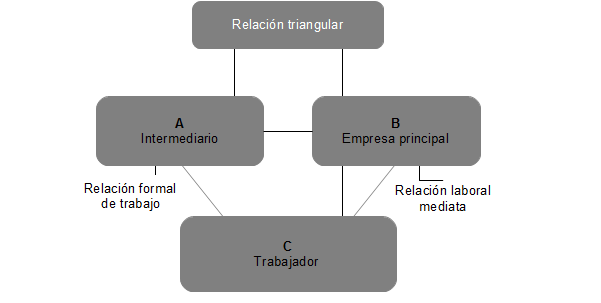
\includegraphics[width=0.5\textwidth]{rel_tri.png}
\caption{Intermediación laboral.}
\end{figure}


\item Esta forma de contratación puede facilitar el desarrollo, por ejemplo, de actividades zafrales, pero en otros casos responde a finalidades fraudulentas, para eludir responsabilidades laborales.
\end{itemize}

\item \textbf{Suministro de mano de obra}

Empresa Suministradora de Mano de Obra: 
\begin{itemize}
\item Se dedica a emplear trabajadores con el fin de ponerlos a disposición de una tercera persona física o jurídica (empresa usuaria), que determine sus tareas y supervise su ejecución.
\item La empresa usuaria requiere atender necesidades temporales, y asume el pago de los créditos que se generen.
\item Ámbitos válidos: trabajo interino, temporal o provisorio (suplencias, trabajo eventual u ocasional, zafral, etc.) para solucionar una necesidad puntual.
\end{itemize}

\textbf{La intermediación es el género y el suministro de mano de obra una especie}.

La diferencia con la intermediación, es que acá la empresa que pide trabajadores tiene que dirigirlos y pagarles, en la intermediación, la empresa intermediaria se encargaba de todo eso.
  
\begin{figure}[H]
\centering
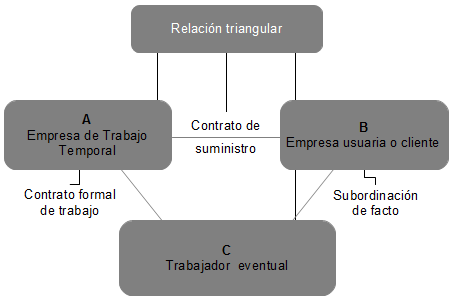
\includegraphics[width=0.5\textwidth]{rel_tri2.png}
\caption{Suministro de mano de obra.}
\end{figure}

\item \textbf{Subcontratación laboral}
\begin{itemize}
\item La subcontratación normalmente es entendida como una expresión o modalidad de la externalización de operaciones.

\begin{figure}[H]
\centering
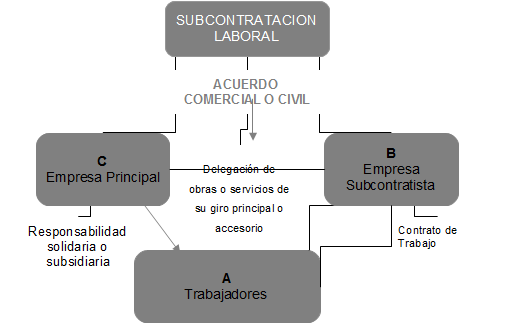
\includegraphics[width=0.5\textwidth]{rel_tri3.png}
\caption{Subcontratación.}
\end{figure}

\item Existe subcontratación cuando un empleador, en razón de un acuerdo contractual, se encarga de ejecutar obras o servicios, por su cuenta y riesgo y con trabajadores bajo su dependencia, para una tercera persona física o jurídica, denominada patrono o empresa principal, cuando dichas obras o servicios se encuentren integrados en la organización de éstos o cuando formen parte de la actividad normal o propia del establecimiento, principal o accesoria (mantenimiento, limpieza, seguridad o vigilancia), ya sea que se cumplan dentro o fuera del mismo”.

\item Este tipo de empresario debe poseer una organización productiva propia, contar con medios materiales y humanos suficientes y ejercer directamente las facultades de organización y dirección del trabajo desarrollado por los trabajadores contratados.

\item En la subcontratación la empresa comitente encarga a la empresa subcontratista la realización de una obra o servicio, que ejecuta con sus propios recursos y bajo su propio riesgo, por lo que los trabajadores no estarán bajo subordinación de hecho en relación a la empresa principal.

\item Rosenbaum se opone a la solución legal de que la subcontratación tenga el mismo régimen de responsabilidad (solidaria o subsidaria) que la intermediación y el suministro, porque en la subcontratación es claro entre quiénes se entabla la relación de trabajo.

\item Por el principio de igualdad de trato, el trabajador suministrado no debe percibir beneficios laborales inferiores a los establecidos por laudos, convenios o decretos del PE para la categoría de trabajadores del giro de la empresa.
\end{itemize} 
\end{enumerate}

\subsection{Régimen de la responsabilidad laboral del empresario principal o la empresa usuaria}

\begin{itemize}

\item Existe un sistema de doble pista\begin{enumerate}
\item[a)] por un lado, un régimen de responsabilidad subsidiario (el trabajador tiene que reclamarle primero al contratista, y si no le pagan va contra el principal) para el caso de que la empresa principal hubiere hecho ejercicio del derecho a exigir información al intermediario, subcontratista o suministrador de mano de obra, en relación al estado de cumplimiento de las obligaciones laborales, previsionales y las correspondientes al seguro de accidentes de trabajo y enfermedades profesionales;

\item[b)] por otro lado, un régimen de responsabilidad solidario  cuando no ejerció efectivamente dicho derecho de información (el trabajador puede ir contra cualquiera de los deudores por la totalidad del monto, sin ningún orden de prelación).

\textbf{Traducción}: Como empresa principal, tenés que asegurarte que contratás un intermediario que encare. Si el intermediario se muere, entonces quedás vos como responsable.

\end{enumerate} 



\item Para ejercer el derecho de información la empresa principal puede requerir datos y documentos de la subcontratista. Tiene que demostrar que hizo un examen diligente. 

\item Cuando el subcontratista, el intermediario o la empresa suministradora no acredite oportunamente el cumplimiento de las obligaciones laborales y previsionales y del seguro de accidentes del trabajo y enfermedades profesionales en la forma señalada, el patrono o empresario principal podrá retener de las obligaciones que tenga a favor de aquél o aquéllos, el monto correspondiente. El mismo derecho tendrá el contratista respecto de sus subcontratistas.

\textbf{Traducción}: Si, como empresa principal, ves que el intermediario que contrataste está haciendo cualquiera, podés cortarle el mambo, y ahí safás.

\end{itemize}

\part{El ordenamiento jurídico laboral}

\chapter{Principios del Derecho del Trabajo}

\section{Protector }

Función: sirve para nivelar desigualdades sustantivas. ¿Cómo? Creando compensaciones jurídicas que “favorecen” al trabajador 

Se materializa a través de 3 reglas
\begin{enumerate}
\item \textbf{In dubio pro operario}: en caso de que una norma pueda entenderse de varias maneras –diferentes significados- o que la valoración de una prueba plantee dudas legítimas, ha de preferirse aquella interpretación o valoración que favorezca al trabajador
\item \textbf{norma más favorable}: cuando existan dos o más normas jurídicas, aún provenientes de distintas fuentes formales, ha de aplicarse siempre la que resulta más favorable al trabajador

\begin{itemize}
\item Las normas establecen “niveles mínimos” en principio inderogables   (Pisos de protección)
\item Nada impide que esos mínimos sean “superados” por otras normas (sobrepujamiento)
\item No opera frente a normas inderogables (de orden público)
ni frente a normas que marcan niveles máximos (topes o techos)
\end{itemize}
\item \textbf{condición más beneficiosa}: al aplicarse una nueva ley, no es posible que se afecten o disminuyan aquellas condiciones más beneficiosas de las que ya goza el trabajador por vía de un contrato, de usos y costumbres o de prácticas profesionales seguidas o admitidas por el empleador
\end{enumerate}

\section{Irrenunciabilidad}

Imposibilidad jurídica del trabajador de privarse voluntariamente de derechos, beneficios o ventajas reconocidas por el derecho de trabajo en su favor. 

Ejemplos:
\begin{itemize}
\item períodos no menores de 10 días en la división de la licencia
\item duración máxima de la jornada
\item aquellas de orden público (no pueden ser modificadas por las partes)
\item nadie puede celebrar contratos de por vida

\end{itemize}

La renuncia a estos derechos se considera ineficaz (sin efectos).

No existe privación de derechos, sino ventajas recíprocas.

\section{Continuidad}

Preferencia del Derecho de Trabajo por los contratos de tiempo indefinido (sin plazo) como forma de asegurarle al trabajador estabilidad en el empleo.

Consecuencias:
\begin{itemize}
\item si en el contrato de trabajo no se estipuló plazo, se presume que es un contrato de duración indefinida 
\item si tiene plazo, pero su ejecución se prolonga más allá, se convierte en un contrato SIN  plazo
\item cuando vence el periodo de prueba y no se rescinde, idem
\item sucesión ininterrumpida de contratos con plazo es vista como un solo contrato SIN plazo
\item no se admite la transformación de un contrato SIN plazo en otro de duración determinada
\item resistencia al despido
\item existe perdurabilidad del contrato de trabajo en casos de sustitución del empleador 
\end{itemize}


\section{Primacía de la realidad}

Lo que interesa más allá de las meras formalidades (apariencias formales) es la verdad de los hechos (verdad material). 
\begin{itemize}
\item En caso de discordancia entre lo que ocurre en la realidad y lo que surge de los documentos o acuerdos, debe darse preferencia a lo que ocurre en la realidad.

\item Bilateralidad del beneficio: favorece tanto al trabajador como al empleador, porque lo que interesa es la verdad.
\end{itemize}
\section{Buena fe}
Tanto el trabajador como el empleador deben dar cumplimiento a las obligaciones derivadas de la relación de trabajo, en forma honesta y correcta y bajo una lealtad recíproca
\begin{itemize}
\item abarca a ambas partes del contrato de trabajo
\item acarca a todos los derechos y obligaciones
\end{itemize}
\section{Razonabilidad}

Parte de la base que todos los hombres han de adoptar conductas racionales (razonables), que responden a patrones de conducta  lógicos y preestablecidos en la vida corriente.
\begin{itemize}
\item tiene un alcance subjetivo (qué es razonable?)
\item sirve para medir la credibilidad de un hecho
\item actúa como límite o freno frente a posibles arbitrariedades
\item tiene una importancia práctica frenete al \textit{ius variandi} (potestad que tiene el empleador de cambiar unilateralmente condiciones no esenciales del contrato de trabajo)
\end{itemize}

\chapter{El ordenamiento normativo laboral.   Las fuentes de derecho.}

El término \textit{fuente del derecho} designa todo lo que contribuye o ha contribuido a crear el conjunto de reglas jurídicas aplicables dentro de un Estado en un momento dado (derecho positivo).

\section{Conceptos previos}
\label{sec:conceptos-previos}

Algunos conceptos sobre fuentes del derecho\footnote{Fuente: http://derecho.utalca.cl/pgs/alumnos/laboral/2.pdf}:

\begin{itemize}
\item \textbf{Fuentes formales del Derecho}: En general, dan cuenta de la forma en que se manifiesta el Derecho. En concreto, son los procedimientos a través de los cuales se producen normas jurídicas, los modos que éstas tienen de manifestarse y los  continentes normativos donde es posible localizar a esas mismas normas una vez que han sido producidas.\\
  Históricamente, en función del poder del que emanan, pueden encontrarse dos grandes vertientes que explican su origen:
  \begin{enumerate}
  \item Corriente \textbf{monista}: El estado es la única fuente productora de derecho:
    \begin{itemize}
    \item Sólo él puede obligar a las personas, ejerciendo el poder de sanción.
    \item Dota de fuerza coercitiva a las reglas de derecho, lo que las diferencia de otras reglas, como las normas morales o las convenciones sociales. Estas últimas se cumplen si se quiere, es a voluntad.
    \end{itemize}
  \item Corriente \textbf{pluralista}: Diversidad de fuentes.
    \begin{itemize}
    \item Se reconoce la existencia de varios centros de poder, de los cuales emanan normas jurídicas.
    \item Habrá normas dictadas por entidades intermedias entre el estado y los individuos, como por ejemplo asociaciones, organizaciones gremiales, etc.
    \end{itemize}
  \end{enumerate}
\item \textbf{Fuentes materiales del Derecho}: Son los factores de diversa índole (políticos, económicos, sociales, científicos, técnicos, etc.) que, presentes en una determinada sociedad en un momento dado, influyen de manera importante en la producción y contenido de una o más normas del ordenamiento jurídico que rige en dicha sociedad.\\
  Ejemplos:
  \begin{itemize}
  \item La Revolución Industrial.
  \item El modelo económico capitalista.
  \item El derecho liberal individualista.
  \item La influencia de la Iglesia Católica (Encíclica Rerum Novarum).
  \item La denominada “cuestión social”\footnote{\url{http://es.wikipedia.org/wiki/Cuestion\_social}}.
  \item La intervención del Estado en las relaciones laborales.
  \item El conflicto de intereses entre trabajadores y empleadores.
  \end{itemize}
\end{itemize}

\subsection{Importancia práctica del derecho laboral}
\label{sec:importancia-practica-del-derecho-laboral}

\begin{itemize}
\item En el campo del DT: La consagración de la autonomía del DT ha ido acompañada por:
  \begin{itemize}
  \item La afirmación de un nuevo poder social con potestad normativa (sindicatos).
  \item Nueva fuente de derecho, no reductible a otras categorías tradicionales.
  \end{itemize}
\item Permite distinguir entre:
  \begin{itemize}
  \item \textbf{Heteronomía}: Fuente formal de normas creadas por los poderes del estado (leyes, decretos, resoluciones, etc).
  \item \textbf{Autonomía colectiva}: Convenios colectivos, laudos\footnote{Valor asignado a algo. Ejemplo: Salario mínimo.} de Consejos de Salarios.
  \end{itemize}
\end{itemize}

\subsection*{Pasaje: Pierre Verge}
\label{pasaje-pierre-verge}

Evolución del pensamiento laboralista en el contexto canadiense:
\begin{enumerate}
\item Reconocimiento de la existencia de \textit{una diversidad de fuentes}: La negociación colectiva y el conflicto colectivo conducen a la estructuración de las relaciones. El conflicto colectivo es generador de normas de trabajo.
  \begin{itemize}
  \item Pluralismo jurídico: La negociación colectiva se coloca junto al derecho etático (hasta entonces sinónimo de derecho civil).
  \item Post-2da Guerra: Reglamentación de la negociación colectiva $\rightarrow$ La negociación colectiva pasa a tener una sanción jurídica: Arbitraje legal.
  \end{itemize}
\item El estado reconoce la naturaleza auténtica de las relaciones colectivas.
  \begin{itemize}
  \item El sindicato es el agente representativo de los trabajadores. Se convierte en sujeto de derechos y obligaciones $\rightarrow$ Accede a la vida jurídica.
  \item El sindicato determina las condiciones de trabajo, los contrato individuales no pueden alterarlas.
  \end{itemize}
\end{enumerate}


\subsection{Fuentes del derecho del Trabajo Como fudamento de la validez de las normas jurídicas}
\label{sec:como-fundamento-de-la-validez-de-las-normas-juridicas}

Estructura piramidal de las normas: La Constitución está por encima de la ley, y ésta prevalece sobre el decreto, y así sucesivamente (en sentido descendente).

La norma superior:
\begin{itemize}
\item Impone conductas.
\item Condiciona a las normas inferiores, controlando que estén de acuerdo con lo que dicta.
\end{itemize}

\section{Proyecciones peculiares en el derecho laboral}
\label{sec:proyecciones-peculiares-en-el-derecho-laboral}

\subsection{Examen estático y dinámico}
\label{sec:examen-estatico-y-dinamico}

\begin{enumerate}
\item \textbf{Jerarquización estática}:
  \begin{itemize}
  \item La escala de normas laborales se estructura de acuerdo con el rango formal de cada disposición:
    \begin{itemize}
    \item Constitución
    \item Tratados y Convenios Internacionales del Trabajo 
    \item Ley ordinaria
    \item Decretos, reglams., actos adms (Normas reglamentarias)
    \item Laudos
    \item Sentencias normativas
    \item Convenios colectivos.
    \item Usos y costumbres
    \end{itemize}
  \end{itemize}
\item \textbf{Jerarquización dinámica}: Entre varias normas vigentes, se elige la más favorable (la que ofrezca mejores condiciones) para el trabajador.
\end{enumerate}

\subsection{Mecanismos de corrección introducidos por el DL}
\label{sec:mecanismos-de-correccion-introducidos-por-el-DL}

\begin{enumerate}
\item \textbf{Conservación de las condiciones más favorables}:
  \begin{itemize}
  \item Si se si se mejoró una situación, esa circunstancia favorable no debería perderse.
  \item \textbf{Terreno individual}: El principio de irrenunciabilidad evita que el individuo elija perder.
  \item \textbf{Terreno colectivo}: El sindicato puede desmejorar un beneficio o eliminar un derecho adquirido. \\
    Por ejemplo: el sindicato puede validar la no aplicación de un aumento salarial (comúnmente llamado descuelgue), a cambio de obtener un compromiso del empleador de no despedir o de no enviar trabajadores al seguro de paro.
  \end{itemize}
\item \textbf{Sobrepujamiento} (criterio de la norma mínima): Las normas laborales fijan niveles mínimos de protección.
  \begin{itemize}
  \item Se puede subir el piso: El sobrepujamiento consiste en que una norma posterior -aún de inferior jerarquía- puede introducir válidamente mejoras sobre el régimen resultante de las normas de jerarquía superior
  \item No se puede bajar el piso: Una norma de jerarquía superior no puede desmejorar un nivel de protección.
  \item Inferiores opacan a superiores: Una norma de cierta jerarquía (p. ej., una ley) deja espacio para ser sobrepujada por una norma de jerarquía inferior (p. ej., un convenio colectivo). Pero la ley no queda derogada, no se produce una ruptura de la jerarquía, sino tan solo el opacamiento de la norma, que es dejada de lado (permanece inaplicada). 
  \end{itemize}
\end{enumerate}

\part{El derecho Internacional del Trabajo}
\label{part:el-derecho-internacional-del-trabajo}

\chapter{Internacionalización del Derecho del Trabajo}
\label{chap:Internacionalizacion-del-Derecho-del-Trabajo}

\section{Origen y nacimiento de la OIT}
\label{sec:origen-y-nacimiento-de-la-oit}

En la conferencia de la Paz de 1919 se propuso estudiar la reglamentación internacional de las condiciones de trabajo.

El nacimiento formal de la OIT se produjo en París con la firma del Tratado de Versailles, en Junio de 1919.

El orden del día de la primer conferencia fue:

\begin{enumerate}
\item Aplicación del principio de la jornada de 8 horas o de la semana de 48 horas.
\item Cuestiones relativas a los medios de prevenir el paro y de remediar sus consecuencias.
\item Empleo de las mujeres:
  \begin{enumerate}
  \item Antes o después del parto.
  \item Trabajo nocturno.
  \item En los trabajos insalubres.
  \end{enumerate}
\item Empleo de los niños:
  \begin{enumerate}
  \item Edad de admisión al trabajo.
  \item Trabajo nocturno.
  \item En los trabajos insalubres.
  \end{enumerate}
\item Extensión y aplicación de convenciones internacionales previamente adoptadas.
\end{enumerate}

\section{Fines de la OIT}
\label{sec:fines-de-la-oit}

\begin{enumerate}
\item \textit{Sentimiento de justicia social}: La idea de que la paz universal y duradera sólo puede fundarse en la justicia social.
\item \textit{Peligro de la injusticia social}: La idea de que existen ciertas condiciones de trabajo que provocan una amenaza para la paz, a causa del descontento que engendran. Implican: injusticia, privaciones y miseria.
\item \textit{Similitud de las condiciones de trabajo en el orden internacional}: La idea de que la desigualdad de las condiciones de trabajo en el orden internacional dificulta el esfuerzo de cada país por mejorar la situación de sus obreros. 
\end{enumerate}

\textbf{Consecuencia}: Necesidad de una reglamentación internacional de las condiciones de trabajo.

\section{Estructura orgánica de la OIT}
\label{sec:estructura-organica-de-la-oit}

Los miembros de la OIT son los Estados.

\subsection{Composición y condiciones de ingreso}
\label{sec:composicion-y-condiciones-de-ingreso}

La calidad de miembro de la OIT se adquiere de 3 modos diferentes:

\begin{enumerate}
\item \textbf{Miembros natos}: Por ser miembros de la OIT el 1/11/45.
  \begin{itemize}
  \item No tienen porque ser miembros de las Naciones Unidas (NU).
  \end{itemize}
\item \textbf{Miembros voluntarios}: Por ser miembros de las NU y comunicar al Director de la Oficina su aceptación de las obligaciones propias de los miembros de la OIT.
  \begin{itemize}
  \item No se lo puede rechazar, ni imponer condiciones $\rightarrow$ La OIT tiene cierta dependencia de las NU.
  \end{itemize}
\item \textbf{Miembros espontáneos}: Por solicitar admisión y ser admitidos por la conferencia general.
\end{enumerate}

\subsection{Órganos de la OIT}
\label{sec:organos-de-la-oit}

Existen 3 órganos fundamentales:
\begin{enumerate}
\item La Conferencia General $\rightarrow$ Deliberante.
\item El Consejo de Administración $\rightarrow$ Directivo
\item La Oficina Internacional del Trabajo $\rightarrow$ Ejecutivo
\end{enumerate}

\subsubsection{La conferencia General}
\label{sec:la-conferencia-general}

Está integrada por Estados, actúan más de 190 miembros.

\begin{itemize}
\item \textbf{Delegados}: 4 representantes de cada uno de los Estados miembros:
  \begin{itemize}
  \item 2 delegados de los gobiernos.
  \item 1 de los empleadores.
  \item 1 de los trabajadores.
  \end{itemize}
\item  \textbf{Carácter tripartito de la OIT}:
  \begin{itemize}
  \item Estado, empleadores y trabajadores.
  \item Partes autónomas, no pierden su identidad ni su independencia para el logro de los objetivos que le son propios.
  \end{itemize}
\item \textbf{Forma de designación}:\\
  \begin{itemize}
  \item Los 2 delegados gubernamentales y sus consejeros técnicos son designados por los gobiernos con entera libertad.
  \item Los delegados no gubernamentales y sus consejeros técnicos deben contar con el acuerdo de las organizaciones profesionales más representativas, siempre que existan tales organizaciones en el país.
  \begin{enumerate}
  \item Se exige contar con el acuerdo del Estado y de las organizaciones profesionales (ninguna basta por sí sola).

    Las organizaciones profesionales designan un candidato, el estado puede rechazarlo, pero no puede proponer otro. Tienen que llegar a un acuerdo.
  \item No se puede cambiar de procedimiento, excepto si no existen organizaciones profesionales en el país.
  \item Debe precisarse el significado de la expresión “organizaciones profesionales más representativas.”:
    \begin{itemize}
    \item Aquellas que aspiren a ejercer la representación en cada sector y que son inevitables en un régimen de pluralidad sindical.
    \item \textit{Organizaciones} se refiere tanto a las organizaciones de empleadores como a las de trabajadores.
    \item Si hay varias organizaciones representativas, todas deben ser tomadas en cuenta por el gobierno, y debe proponerse buscar el acuerdo con todas (basta el intento, es complicado lograr un acuerdo).
    \item Cada país debe determinar cuales son las organizaciones más representativas al momento de la designación.

      Criterios:
      \begin{enumerate}
      \item Número de afiliados.
      \item Tradición del sindicato.
      \item Obra que desarrolla.
      \item Independencia del mismo.
      \item Autenticidad de la labor de defensa de los intereses profesionales confiados a su custodia.
      \end{enumerate}
    \item Una organización representativa debe actuar en un clima de \textbf{libertad}.
    \item Una vez comunicada la designación de los delegados y consejeros técnicos a la Oficina Internacional del Trabajo, ella no puede revocarse.
    \end{itemize}
  \end{enumerate}
\end{itemize}
\item \textbf{Facultades}:
  \begin{enumerate}
  \item De orden interno: verificación de los poderes de los delegados, determinar el lugar de la Conferencia, inclusión en el orden del día de uno o más puntos.
  \item De orden constituyente: enmendar la Constitución por mayoría de 2/3 de votos emitidos por los delegados presentes.
  \item De orden electivo: elige los 4 miembros de la Mesa y los miembros electivos del Consejo de Administración.
  \item De orden deliberante: tarea fundamental que culmina en la aprobación de convenios y recomendaciones, así como de resoluciones.
  \item De orden administrativo: consideración de la Memoria del Director General, aprobación del presupuesto y del prorrateo y recaudación de las contribuciones.
  \item De orden reglamentario: reglamenta su propio funcionamiento.
  \end{enumerate}
\end{itemize}

\subsubsection{El consejo de administración}
\label{sec:el-consejo-de-administracion}

Constituye el Poder Ejecutivo de la OIT.

\begin{itemize}
\item \textbf{Integración tripartita}: 56 delegados. El número de delegados gubernamentales equivale al número total de delegados de empleadores y trabajadores:
  \begin{itemize}
  \item 28 representantes de los gobiernos, 
  \item 14 de los empleadores.
  \item 14 de los trabajadores.
  \end{itemize}
\item \textbf{Designación de los integrantes}: Cada uno de los 3 grupos de la conferencia (gobiernos, empleadores, trabajadores) se convierten en colegios electorales:
  \begin{itemize}
  \item Los delegados gubernamentales designan 18 Estados cuyos gobiernos tendrán, cada uno, derecho a nombrar 1 miembro gubernamental en el consejo. Los otros 10 son designados por los miembros de mayor importancia industrial, los cuales no participan en la designación de los 18 anteriores. Se eligen Estados, los cuales a su vez designan una persona física para representarlos. El Consejo de Administración determina, cada vez que sea necesario, cuáles son los miembros de mayor importancia industrial.
  \item El grupo patronal y el grupo trabajador designan 14 miembros titulares y 10 miembros adjuntos. Se eligen directamente personas.
  \item La elección se hace cada 3 años, durante la reunión de la Conferencia, por voto secreto y en forma nominal, por un número de votos superior a la mitad de los votos emitidos por los miembros del colegio electoral presentes en la reunión.
  \end{itemize}
\item \textbf{Facultades}: 
  \begin{itemize}
  \item Fijación del orden del día
  \item Control del cumplimiento de las obligaciones por los Estados miembros.
  \item Gestión económica de la OIT.
  \item Designación del Director General.
  \end{itemize}
\end{itemize}

\subsubsection{La Oficina Internacional del Trabajo}
\label{sec:La Oficina Internacional del Trabajo}

Órgano ejecutivo.
Secretariado. Es la única que posee personal o funcionarios permanentes.

\begin{itemize}
\item \textbf{Director General}: 
  \begin{itemize}
  \item Al frente de toda la Oficina Internacional del Trabajo debe existir un jerarca responsable, que es el Director General.
  \item Nombrado por el Consejo de Administración. No se exige ninguna mayoría. Siempre se lo ha nombrado por unanimidad.
  \item No tiene plazo de duración, por lo que posee carácter permanente. Costumbre: designación por plazos de 5 años renovables indefinidamente.
  \end{itemize}
\item \textbf{Funciones}: Encargada de asegurar el funcionamiento regular de la OIT. Debe cumplir todas aquellas funciones que la Conferencia o el Consejo consideren conveniente encomendarle o que su Director entienda incluida dentro de su misión.
\end{itemize}

\section{Las normas internacionales}
\label{sec:las-normas-internacionales}

Tratado de Versailles: se pretendió crear un poder legislativo internacional, aunque limitado en sus alcances. La OIT, sin embargo, no es un organismo supranacional. Se llegó a una solución de transacción: la creación de 2 tipos de normas fundamentales: 

\begin{enumerate}
\item Los convenios internacionales (CIT).
\item Las recomendaciones (RIT).
\end{enumerate}

Los CIT y las RIT constituyen siempre normas mínimas.
\begin{table}
\begin{tabular}{|c||p{6cm}|p{6cm}|}
  \hline
  & \textbf{CIT} & \textbf{RIT}\\
  \hline
  \hline
  \textbf{Concepto} & Textos aprobados por 2/3 de votos en una Conferencia Internacional del Trabajo, que una vez ratificados por las autoridades competentes de cada Estado, entran a regir las relaciones laborales producidas en el mismo. Se reservan para los temas importantes, susceptibles de una definición y acción precisas. & Textos aprobados por 2/3 de votos en una Conferencia Internacional del Trabajo, comunicados a los Estados miembros, para que procuren llevarlos a la práctica mediante la aprobación de leyes o de  cualquier otra manera.\\
  \hline
  \textbf{Trámite} & Deben someterse a la autoridad competente para su ratificación & No se ratifican. No requieren acto posterior alguno de los E miembros.\\
  \hline
  \textbf{Contenido} & Contienen normas. Una vez ratificadas rigen directamente en el país respectivo. & Sólo contienen guías u orientaciones para la acción legislativa nacional de los E.\\
  \hline
  \textbf{Finalidad} & Obligan a que los Estados ratificantes respeten y observen las cláusulas contenidas en ellos. & Procuran sentar principios inspiradores y orientadores de la política nacional de los E.\\
  \hline
  \textbf{Repercusión} & Si un E aprueba el contenido de un CIT basta la ratificación para que rija efectivamente en el territorio del país. & Si un E apoya una RIT debe dictar una ley especial que materialice las disposiciones de la misma.\\
  \hline
  \textbf{Obligaciones} & El E tiene la obligación de hacer cumplir su contenido y queda sometido a los procedimientos de contralor (queja y reclamación) & El E sólo debe informar periódicamente sobre el estado de su legislación respecto de los asuntos tratados en las RIT\\
  \hline
\end{tabular}
\caption{Diferencias entre RIT y CIT}
\label{tab:rit-cit}
\end{table}
\newpage
\section{Material complementario}
\label{sec:material-complementario}

\subsection{Declaración del a OIT}
\label{sec:declaracion-de-la-oit}

Los miembros de la OIT deben encarar con:
\begin{enumerate}
\item La libertad de asociación y la libertad sindical y el reconocimiento efectivo del derecho de negociación colectiva; 
\item La eliminación de todas las formas de trabajo forzoso u obligatorio;
\item La abolición efectiva del trabajo infantil; y
\item La eliminación de la discriminación en materia de empleo y ocupación. 
\end{enumerate}

Deben ayudar (aportes técnicos, asesoramiento) a los miembros que necesitan ayuda, para crear un entorno favorable de desarrollo económico y social.

Basicamente, cumplir con todo, y hacerlo de buena fe.

\subsection{Pacto mundial de empleo}
\label{sec:pacto-mundial-de-empleo}

“La crisis global requiere de soluciones globales”

“Las respuestas a la crisis no deben tener carácter puntual y ser aplicadas temporalmente, para luego regresar a funcionar como de costumbre lo antes posible. Es esencial seguir adelante con el Programa de Trabajo Decente para apoyar la recuperación económica, evitar las crisis sociales y del mercado de trabajo, y promover la cohesión social”.

Al trabajar en torno a un Pacto Mundial para el Empleo, los mandantes de la OIT podrían realizar una importante contribución a la coherencia global en torno a estos temas. (...) abordando así los factores clave que alimentaron la crisis y sentando las bases de una economía más sostenible.


\part{Relaciones jurídicas individuales del trabajo}

\chapter{Relación de trabajo y subordinación}
\section{Reseña de algunas nociones preliminares}

La prestación del trabajo que se pueden dividir en diferentes tipos contractuales. Algunos pueden regirse por el Derecho Civil (arrendamiento obra o de servicios), y otros por el \textbf{DT}. Pero existe otra clasificación mucho más general: \textbf{la prestación de actividades}. Incluye (además del arrendamiento de servicios y obra y el contrato de trabajo), el mandato, transporte, agencia, depósito, sociedad, etc.\\

El contrato de trabajo ha ido evolucionando desde el campo de las relaciones civiles hasta encontrar su \textbf{fisionomía propia y autónoma}, en el ámbito del \textbf{Derecho del Trabajo}. El contrato de trabajo es independiente del resto y está sometido a un régimen jurídico original y muchas veces opuesto al de otros contratos semejantes que pertenecen al derecho civil o mercantil.
Lo característico es que en la relación de trabajo, el trabajador se encuentra frente al empleador en una posición de \textbf{dependencia personal}, definido \textit{ab initio} como una sujeción jurídica del primero, ya que el trabajador debe ajustarse o acatar las órdenes del empleador.

En nuestro país la figura del contrato de trabajo tuvo aparición tardía, lo cual proyecta 2 consecuencias fundamentales:
\begin{itemize}
	\item Sólo en virtud de un contrato de trabajo tendrá aplicación el \emph{estatuto legal propio del trabajador asalariado}: condiciones de trabajo, pago de salarios, ruptura del contrato, etc.
	\item Para el Derecho del Trabajo, todo lo que no esté comprendido o alcanzado por las notas propias de un régimen de subordinación, \emph{queda al márgen de su protección} y por tal razón, el trabajador autónomo o indpendiente posee una ubicación marginal, semejante a la de la figura del empleador.
\end{itemize}

Es fundamental conocer si la relación entre sujetos de derecho es de \textbf{dependencia} o \textbf{subordinación}, ya que es un punto determinante de la vigencia conceptual del DT.

\subsection{La subordinación}

3 acepciones posibles:
\begin{enumerate}
	\item \textbf{Subordinación técnica}: el empleador dirige efectivamente las tareas del trabajador, indica explícitamente la forma en q se debe desarrollar la tarea, vigila inmediata y permanentemente. El empleador posee el conocimiento necesario y suficiente de las tareas. Esta modalidad tiende a desaparecer, sustituyéndose por otra donde el empleado está más capacitado técnicamente que su empleador para la tarea que desarrolla.
	\item \textbf{Subordinación económica}: el trabajo es la única fuente de subsistencia del trabajador.
	\item \textbf{Subordinación jurídica}: el la potestad del empleador de dirigir una cierta actividad del trabajador cuando lo crea necesario. Queda comprendida la facultad del empleador de dirigir la empresa, dando órdenes e instrucciones a los trabajadores, organizando el funcionamiento de la misma, ejerciendo el contralor o vigilancia de los procesos operativos. Se trata de un conjunto de potestades reconocidas al empleador: poderes directivo, reglamentario, disciplinario, etc.
\end{enumerate}

\textbf{La noción de subordinación se caracteriza por su complejidad, constituyéndose en un concepto único que abarca las 3 modalidades mencionadas. Los criterios expuestos no son válidos de forma aislada, sino que deben considerarse actuando conjuntamente, constituyendo un \textit{haz concordante susceptible de crear convicción}}

\subsection{Otros elementos caracterizantes}
Junto a la subordinación, la doctrina ha perfilado otras características configurativas del \textit{trabajo} como objeto del Derecho Laboral.

\subsubsection{La actividad personal o prestación personal del servicio}
En muchos contratos se exige la prestación personal, pero en el trabajo es el objeto principal. Este trabajo es \textit{intuitu personae} respecto del trabajador lo cual excede el marco patrimonial (como por ejempolo el deber de disciplina, lealtad, buena fé, etc.).
La prestación de esta actividad no necesariamente es de forma constante, sino que es posible su presencia potencial (estar a la orden).

\subsubsection{La remuneración u onerosidad}
Consecuencia ineludible de la actividad personal y subordinación. Es la contraprestación recibida por el trabajador por poner su energía a la orden del empleador.

\subsubsection{La durabilidad}
\begin{itemize}
\item La voluntad del empleado y del empleador de vincularse uno con otro de manera durable". 
\item No es recogido como nota esencial. 
\item La durabilidad no es sinónimo de perpetuidad, sino que en realidad pone el acento en que la relación de trabajo no es fugaz o esporádica, sino que tiene vocación de permanencia.	
\end{itemize}

\subsubsection{La ajenidad}
\begin{itemize}
	\item ALONSO OLEA: \textit{Constituye el verdadero elemento típico del contrato de trabajo}
	\item Acto de cesión originario. Si bien los frutos emanan del trabajo del obrero, \textit{nacen} en el patrimonio del empleador
	\item Esta ajenidad en el resultado, condiciona también la ajenidad en los riesgos.
	\item MONTOYA MELGAR: \textit{la utilidad patrimonial del trabajo se atribuye, en realidad, a persona distinta del propio trabajador}
	\item SARTHOU: \textit{El manejo de la idea de la ajenidad resulta de utilidad como criterio complementario al de subordinación, para despejar dudas frente a supuestos que ingresan en zonas grises en cuanto a su real determinación}
\end{itemize}

\subsection{Algunos indicios manejados por la jurisprudencia}

Se exponen algunos criterios tendenciales que la jurisprudencia ha desarrollado al efecto de determinar o descartar la presencia de una relación de trabajo.\\

Atendiendo al principio de primacía de la realidad, los fallos privilegian lo ocurrido en la práctica, aún frente a lo emandado de las formas.\\
\textbf{\textit{En caso de discordancia entre lo que ocurre en la práctica y lo que surge de los documentos, debe darse preferencia a lo primero}}.

\textit{No es el empleador el que debe atribuir la calidad de empleado; ésta surge de la naturaleza de los hechos de la relación jurídica que la configura, independientemente de la interpretación más o menos tendenciosa de los interesados}\\

Indicios para determinar relación laboral:
\begin{itemize}
	\item Se analiza directamente el vínculo de subordinación, comprendiendo la sujeción a los \textbf{poderes de organización}, \textbf{dirección}, \textbf{control}, y \textbf{fiscalización} que ostenta el empleador
	\item Se estudian elementos complementarios a la subordinación, como la \textbf{continuidad}, la \textbf{profesionalidad}, la \textbf{exclusividad}, la \textbf{ajenidad}, y la \textbf{inserción} en la organización
	\item Indicios que operan a través de una simple función de refuerzo de los anteriores, pero que carecen de fuerza individual, como por ejemplo el \textbf{cumplimiento del horario}, forma y modalidad de \textbf{retribución}, incidencia subjetiva del \textbf{riesgo} y el \textbf{objeto y cumplimiento de obligaciones formales} frente a organismos de previsión, fiscales o registrales.
\end{itemize}

\chapter{Ni idea el título de este capítulo}
\section{Obligaciones y derechos de las partes del contrato de trabajo}
Obligaciones vienen o de la ley o del contrato (o también de la equidad, el uso o la ley).
En Uruguay no hay un código de trabajo que lo regule de forma orgánica

\subsection{Obligaciones del trabajador}
\begin{itemize}
	\item \textbf{Prestación de servicio}: obligación de obediencia, fidelidad, colaboración y obligaciones morales. Algunos dicen que el trabajador está obligado a estar a la orden del empleador, no requiriéndose la efectiva prestación de servicios. Recordar que la prestación de servicio es personalísima e intransferible.
	\item \textbf{En condiciones pactadas de lugar y tiempo}. Las condiciones pactadas delimitan responsabilidades. Importante para el trabajador (para saber bien sus responsabilidades) y para el empleador (para delimitar su potestad disciplinaria)
	\item \textbf{Con eficiencia normal}. Asegurar especificación de rendimiento. El trabajador debe cumplir las tareas con una \textbf{diligencia} normal. Para medir el rendimiento comúnmente se utiliza la costumbre basada en experiencia: el tiempo promedio en que usualmente se realiza cierta tarea. Se podrían tomar tiempos y establecer estándares...
	\item \textbf{Con el debido manejo de materiales máquinas e instrumentos}. Cuidado y conservación de herramientas, materias primas, objetos. Trabajador es responsable por ellos.
	\item \textbf{Obligación de obediencia}. Fundada en la subordinación  jurídica del contrato de trabajo. Obedecer las ordenes impartidas con límites, razonabilidad, seguridad e higiene, y el límite de los derechos inespecíficos del trabajador. Las excepciones al deber de obediencia son actos ilícitos, cosas peligrosas, cosas imposibles de cumplir y ordenes de un subordinado que contradigan ordenes de un superior.
	
	\item \textbf{Obligación de fidelidad} (lealtad). Proyección al contrato de trabajo del principio de la buena fe. Obligación comunitaria y no contractual.
	Esta obligación se traduce en tres deberes negativos o de abstención: 
	\begin{enumerate}
		\item No aceptar gratificaciones, regalos o ventajas de terceros que trabajan con el empleador sin su conocimiento, exceptuando la propina.
		\item No revelar secretos de los que haya tenido conocimiento en ocasión del trabajo. Es común el establecer clausulas de confidencialidad.

		Conocimientos $\neq$ secretos: Los primeros son formación profesional y los segundos son datos reservados que, de revelarse generan perjuicio a la empresa.
		\item No lo pone.... dice q hay 3 deberes pero pone 2...
	\end{enumerate}
	\item \textbf{No realizar concurrencia desleal ni colaborar con quienes lo hagan}. Concurrencia es realizar actividades parecidas  a lo que se realiza en el trabajo, de modo que perjudiquen al empresario, compitiendo real o potencialmente.
	\item \textbf{Obligación moral}. Consideración tanto al empleador como a sus superiores y compañeros de trabajo.
	Prohibir gestos y comportamientos. En gral. un trabajador se integra a un grupo y debe adaptarse a una estructura en vez de imponer su parecer. 
	Estas obligaciones se mantienen en tanto en el ámbito de trabajo como fuera de él.
\end{itemize}

\section{Invenciones del trabajador y derechos de la propiedad intelectual}
En este tema, Pla1 distingue tres clases de invenciones: 
\begin{itemize}
	\item \textbf{Las invenciones de servicio}. Realizadas por personas especialmente contratadas para investigación.
	\item \textbf{Las invenciones de empresa o de establecimiento o explotación}. Surgen en el transcurso natural de las actividades de la empresa o establecimiento, pero en cuyo surgimiento ha predominado el proceso, las instalaciones, los procedimientos y los métodos de la empresa.
	\item \textbf{Las invenciones libres}. Son las derivadas de una influencia predominante del ingenio, el talento y lo creatividad del trabajador.
\end{itemize}
El derecho a las invenciones es inalienable e imprescriptible, se transmite a sus herederos y se protege mediante patentes.
No se puede renunciar a este derecho.
El estado no garantiza el mérito, la novedad ni la calidad del inventor.\\

No se consideran invenciones:
\begin{enumerate}
	\item Descubrimientos, teorías científicas, métodos matemáticos.
	\item Plantas y animales exceptuando miroorganismos y procedimientos biológicos para producción de plantas o animales
	\item Esquemas, planes, reglas, principios o métodos comerciales, contables, financieros, educativos, de sorteo o fiscalización
	\item Obras literarias, artísticas y científicas
	\item Programas de computación
	\item $\neq$ formas de reproducir información
	\item Material biológico y genético como existe en la naturaleza.\\
\end{enumerate}
No son patentables:
\begin{enumerate}
	\item Métodos de diagnóstico, terapéuticos y quirúrgicos para el tratamiento de personas o animales.
	\item Las invenciones contrarias al orden público, las buenas costumbres, la salud pública, la nutrición de la población, la seguridad o el medio ambiente.
\end{enumerate}

\subsection{Invenciones realizadas durante una relación de trabajo}
Si la invención se da bajo un contrato donde el objeto total o parcial es la investigación, el derecho de la patente es del empleador. Si el aporte del trabajador es muy grande y excede el contrato, tendrá derecho a remuneración extra.\\

Si el trabajador realiza un invento relacionado con su trabajo y la empresa juega un papel importante, tanto en la capacitación del trabajador o en la prestación de medios, entonces el trabajador debe notificar por escrito al empleador quien tiene 90 días para demostrar su interés. En este caso comparten el derecho.

En cualquier otro tipo de invención, el derecho pertenece al inventor.\\

Las patentes duran 20 años desde q se solicita.

\subsection{Requisitos y procedimientos de concesión de patentes}
Impide que terceros realicen sin autorización:
\begin{enumerate}
	\item Sobre un producto: fabricarlo, ofrecerlo, venderlo, utilizarlo, importarlo y almacenarlo para alguno de estos fines.
	\item Sobre un procedimiento:usarlo y hacer cualquiera de las cosas del punto anterior con el producto resultado del procedimiento.
\end{enumerate}

Los derechos patrimoniales de una patente pueden ser transferidos o cedidos por su titular o causahabientes por sucesión o pacto.

La Dirección Nacional de la Propiedad Industrial es el órgano competente.

Se prohíbe establecer licencias contractuales que produzcan efecto negativo en competencia, competencia desleal o hagan posible un abuso por el titular. Se prohiben también las que producen efectos perjudiciales para el comercio, condiciones de retrocesión, impedimentos a la impugnación de la validez de las patentes, limitaciones al licienciatario en planos comercial o industrial, limitaciones a la exportación a países con acuerdo de zona de integración económica y comercial.

\subsection{Disposiciones penales}
El que no haga caso se liga de 6 meses de prisión a 3 años de penitenciaría.
La pena será de quince meses de prisión a cuatro años de penitenciaría cuando se agrave por alguna de estas cosas:
\begin{itemize}
	\item Haber sido dependiente del titular de la patente o de un licenciatario de la misma.
	\item Haber obtenido de éstos el conocimiento de las formas especiales de realización del objeto patentado.
\end{itemize}

\section{Poder de dirección y sus distintas proyecciones. Facultades disciplinarias.}

MATERIAL DE LECTURA SEPARADO!!! ¿¿¿DE DONDE LO SACO??? tan pa la joda...

\section{Tecnologías y derecho a la intimidad}
\subsection{Tratamiento de datos personales de los trabajadores}
Ausencia de un marco normativo especial y uniforme provoca inseguridad jurídica.\\

En esta materia la constitución de Uruguay está bastante bien pero la legislación no.\\

Línea al re pedo.\\

El derecho a la intimidad es un derecho fundamental inespecífico que tiene el trabajador como ciudadano. La subordinación puede limitar este derecho. El poder de vigilancia y contralor del empresario sobre el trabajador vulnera el derecho a la intimidad cuando se extralimita, cuando los medios electrónicos controlan al trabajador y no a la actividad que este realiza.\\

\subsubsection{Régimen legal de solicitud de datos personales del trabajador: condiciones y límites}
En 2004 se aprueba una ley sobre protección de datos personales de carácter comercial. Se exceptúan de esta ley el tratamiento de datos no comerciales, como:
\begin{itemize}
	\item Datos personales originados al emitir opinión, informar, datos de encuestas, estudios de mercados, etc.
	\item Datos sensibles a la privacidad de las personas: origen racial, étnico, preferencias políticas, religiosas, filosóficas o morales, afiliación sindical, referente a salud física o a sexualidad y toda otra zona reservada de libertad individual.
\end{itemize}
En 2008 se deroga la ley anterior y se hace otra que comprende  todos los datos personales de los trabajadores y se proyecta al ámbito de las relaciones de trabajo, aunque no sea específica de las rel. laborales.
La ley dice algunas cosas destacables:
\begin{itemize}
	\item Protección de datos personales como un derecho humano inherente a la persona humana.
	\item Se puede obtener toda la información de uno mismo presente en las bases de datos públicas o privadas
	\item Se puede exigir la rectificación, actualización, inclusión o supresión de datos personales si se constata errores o falsedades
\end{itemize}

\subsubsection{Almacenamiento de datos: reglas, su uso y divulgación, datos que están vedados a toda solicitud de información}
Ya se mencionaron los principios de:
\begin{itemize}
	\item \textbf{Finalidad}: usar los datos solo para lo que fueron pedidos.
	\item \textbf{Reserva}: utilización reservada
	\item \textbf{Responsabilidad}: el responsable de la base de datos responde ante violación de ley
\end{itemize}
Ninguna puede ser obligada a proporcionar \textbf{datos sensibles} (origen racial, étnico, pref. políticas, sindicatos, salud, sexualidad)\\

\subsubsection{Derecho de resistencia del trabajador a brindar la información requerida}
Lo mismo q lo anterior. Si el trabajador no quiere, no tiene por qué dar datos sensibles, puediendo entablar una acción judicial...

\subsection{Uso de internet y correo electrónico}
El e-mail, los SMS, el GPS y las computadoras adaptadas a la producción hacen que se extremen los controles sobre el trabajador retomando el concepto de productividad y desplazando espacios del trabajador inactivo o a la orden.\\

En Uruguay se sostiene que el control sobre el trabajador no puede ser ilimitado. El empleador puede conocer en tiempo real los movimientos del computador del trabajador, lo cual roza con el derecho de privacidad del trabajador.\\

Sobre el correo electrónico, hay quienes dicen que al ser una herramienta de trabajo, se puede monitorearlo y además es sancionable si se usa para fines no laborales. Otros sostienen que el monitoreo del c.e. vulnera derechos fundamentales, como de la intimidad, libertad, etc.\\
La interceptación de las comunicaciones solo es válida si es realizada por la autoridad competente a petición de la Justicia. En Uruguay no se pueden hacer pesquisas secretas por mandato constitucional. Se considera el correo electrónico como un mensaje de persona a persona y su intercepción es un delito penal.\\

\textbf{Se presume que el contenido de la comunicación es secreto para todos aquellos que no participan de la misma, ni está destinada directa o indirectamente.}\\

\textbf{El avance de la tecnología y sus diversas manifestaciones requieren una reformulación de los medios que se encuentran al alcance de los representantes (sindicales) para el cumplimiento de sus funciones}

\subsection{Cámaras, micrófonos y otros instrumentos de control}

Dichos instrumentos son de amplia utilización en el interior de la mayoría de las empresas y atentan contra la intimidad de los trabajadores.\\

No es posible colocarlos en vestuarios, lugares de esparcimiento, comedores y lugares de reuniones sindicales.\\

Es posible saber muchas cosas de una persona, teniendo en cuenta pagos con tarjeta, utilización de transporte colectivo, alojamiento en hoteles, cámaras de seguridad de calles, bancos, estadios, control satelital del vehículo, revisación electrónica de equipaje, medición de temperatura, etc. Toda esta tecnología atenta contra la privacidad de las personas.\\

Están prohibidas las  listas negras de trabajadores con rango legal, pero con referencia a derechos inherentes a la personalidad humana.\\

\section{Teletrabajo}
\subsection{Desarrollo del teletrabajo}

\begin{itemize}
	\item entre un 16\% y  un 22\% de los uruguayos tienen acceso a internet, según datos obtenidos antes del 2006
	\item Existen unos 3000 trabajadores a distancia en diversas profesiones.
\end{itemize}

\subsection{El teletrabajo como nueva oportunidad laboral y expresión de flexibilidad en el mercado de trabajo.}
Forma atípica de contrato de trabajo.\\

En definitiva, el teletrabajo es examinado como el resultado de la aplicación de la \textbf{tecnología informática} pero además como la manifestación de los cambios en la organización del trabajo, destinados a incrementar los procesos de \textbf{flexibilización} en el derecho del trabajo, que permiten eludir o reducir la aplicación de la normativa laboral y de seguridad social.

\subsection{El teletrabajo en el derecho del trabajo y en la seguridad social: normas, criterios prácticos, convenios colectivos, jurisprudencia}
Se debe distinguir entre:
\begin{enumerate}
	\item Teletrabajo autónomo e independiente
	\item Teletrabajo pero en lugares distintos al domicilio del trabajador (telecentros)
	\item Teletrabajo subordinado  realizado en el domicilio del trabajador
\end{enumerate}
En este último se concentra el estudio de Raso Delgue, quien afirma que no se debe aplicar la normativa nacional sobre trabajo a domicilio.\\

Hay un convenio sobre trabajo a domicilio de la \textbf{OIT} donde se aplica una definición que permite incluir al teletrabajador con actividad en su domicilio dentro del convenio. Pero este convenio no ha sido ratificado por nuestro país.\\

El tema es que si no se considera como un "trabajador a domicilio (y no se le aplican las leyes especiales), deberá regirse entonces por las leyes de los trabajadores normales. Esta es la posición que adopta la decisión judicial en 2004. En algún momento se pretendió disfrazar como un contrato de arrendamiento de servicios pero debe tener naturaleza laboral.\\

Hay varios aspectos donde el trabajador a domicilio se asemeja al teletrabajador. Por ejemplo en problemas de salud y seguridad laborales, vinculados al aislamiento del trabajador en su domicilio.\\

El contralor que puede ejercer el empleador a través de la tecnología que se utiliza, es de tal intensidad, que puede resultar más grave que el que presentan los trabajadores instalados en el local de la empresa.\\

\chapter{FALTA}
%11
\chapter{FALTA}
%12
No tenemos material sobre este capítulo.
Jodámosnsoss.s

\part{Relaciones colectivas del trabajo}
\label{part:relaciones-colectivas-de-trabajo}

\chapter{Derecho Colectivo del Trabajo (DCT)}

\section{Origen histórico del DCT}
\label{sec:origen-historico-del-dct}

El origen, en términos históricos, debe encontrarse en la Revolución Industrial.

Al aparecer la "gran fábrica", al masificar y agrupar al trabajador en ese conglomerado, que implicaba la convivencia diaria, de 16 o más horas, con salarios insuficientes y de trabajo, de higiene y de seguridad laboral indecorosas, se provocó un efecto inevitable:
\begin{itemize}
\item Una unión consciente y voluntaria de los trabajadores para actuar frente al empleador.
\end{itemize}

\section{Funciones del DCT}
\label{sec:funciones-del-dct}

Objetivos:
\begin{itemize}
\item presionar al empleador (con el uso de medidas de presión y acciones de fuerza);
\item equilibrar las posiciones de poder (por la fuerza del número y de la unión organizada);
\item establecer una nueva forma de negociación (colectiva, en vez  de individual);
\item bilateralizar la regulación de las condiciones de trabajo y empleo (“el fin del absolutismo patronal”, según De Ferrari)
\end{itemize}

\textbf{Funciones protectoras}:
\begin{enumerate}
\item Organizativa (Autarquía\footnote{autosuficiencia, autogobernarse.} sindical)
\item Normativa (Autonomía colectiva)
\item De garantía (Autotutela)
\end{enumerate}

\textbf{Funciones complementarias}:
\begin{enumerate}
\setcounter{enumi}{3}
\item Gobierno de las relaciones laborales
  \begin{itemize}
  \item Conjunto de actores (colectivos):
    \begin{itemize}
    \item Sindicatos.
    \item Empresa u organizaciones de empleadores.
    \end{itemize}
  \item Sistema de creación de normas: Negociación colectiva.
  \item Factor de manejo, administración y gobierno del conjunto de:
    \begin{itemize}
    \item relaciones obrero-patronales.
    \item relaciones que se generan a propósito de la actividad económica.
    \end{itemize}
  \end{itemize}
\item Gobierno del sistema social en su conjunto: Gobierno+Empleadores+Sindicatos desarrollan funciones que rebasan las relaciones obrero-patronales, apuntando a acuerdos macroeconómicos, sociales y jurídicos.
\end{enumerate}

\section{Denominación}
\label{sec:denominacion}

Algunos prefieren \textit{Derecho Sindical}, otro \textit{Derecho Colectivo del Trabajo}.

Breve fundamento de una u otra:

\begin{itemize}
\item \textit{Derecho Sindical}:
  \begin{enumerate}
  \item La calificación como derecho \textit{colectivo} constituye un término impreciso.
  \item La huelga y la negociación colectiva derivan del Sindicato, y no se justificarían sin la existencia del sindicato.
  \item La expresión \textit{Derecho Sindical} es sustancialmente correcta, ya que del lado de los trabajadores \textit{siempre} tiene que haber un sindicato (del lado del empleador puede ser un patrón individual).
  \end{enumerate}
\item \textit{Derecho Colectivo del Trabajo}:
  \begin{enumerate}
  \item Es la denominación más generalizada.
  \item Resulta  comprensiva de aspectos no estrictamente sindicales, aunque derivados de lo sindical (Ermida).
  \item Es más aséptica (el término sindical tiene un arrastre histórico negativo)
  \end{enumerate}
\end{itemize}

\section{Particularismos del DCT}
\label{sec:particularismos-del-dct}

\subsection{Elementos típicos}
\label{sec:elementos-tipicos}

\begin{itemize}
\item \textbf{Sujetos}:
  \begin{enumerate}
  \item \textit{Esencialidad del sujeto colectivo trabajador}: Mientras en el derecho individual de trabajo, los sujetos principales son el trabajador y el empleador individualmente considerados, en el DCT al menos uno de los sujetos es siempre un grupo de trabajadores, el que actúa como representante de una comunidad definida de intereses. \\
    Puede ser una asociación organizada y estructurada (sindicato), una unión, un agrupamiento espontáneo, etc.
  \item \textit{Inesencialidad del sujeto colectivo empleador}: La pluralidad es esencial sólo en lo que refiere a la estructuración de los trabajadores, ya que constituyen el sujeto débil de la relación de trabajo.
  \item \textit{El Estado}: La esencialidad del estado depende del enfoque. Oscila entre dos extremos:
    \begin{itemize}
    \item En los sistemas de mayor autonomía, la importancia recae en los trabajadores y en los empleadores.
    \item En los sistemas de mayor intervención, el Estado restringe el ámbito para las relaciones autónomas de los actores sociales (determina qué materias pueden ser objeto de negociación, potestad de habilitar a un sindicato, regula el conflicto colectivo, etc.).
    \end{itemize}
  \end{enumerate}
\item \textbf{Contenidos}:
  \begin{itemize}
  \item Crea estructuras encaminadas a la fijación de las condiciones de trabajo. No hay relaciones de trabajo directas, individuales. (contrato $!=$ convenio colectivo).
  \item Implica medios e instrumentos diferentes.
  \end{itemize}
\item \textbf{Intereses}:
  \begin{itemize}
  \item Económicos: Fundamentalemente salariales.
  \item Indivisibles: Pertinentes a una colectividad dada.
  \item Genéricos: Se aplican, de modo abstracto y general, a un conjunto de personas.
  \end{itemize}
  El interés colectivo no constituye la mera suma de intereses individuales, sino la combinación de esos intereses.
\item \textbf{Medios o instrumentos}:
  \begin{enumerate}
  \item El sindicato.
  \item La negociación colectiva (permite crear normas de carácter extraetático).
  \item La huelga para proteger los intereses colectivos (uso legal de la fuerza).
  \end{enumerate}
\end{itemize}

\subsection{Institutos del DCT}
\label{sec:institutos-del-dct}

Triangularidad del derecho colectivo del trabajo:

\begin{quote}
\begin{quote}
\begin{quote}
\begin{verbatim}
        Sindicato
           .
          / \
         /   \
        /     \
       /       \
      .---------.
Convenio       Huelga
colectivo
\end{verbatim}
\end{quote}
\end{quote}
\end{quote}

De manera más general:
\begin{quote}
\begin{quote}
\begin{quote}
\begin{verbatim}
        Autarquía
           .
          / \
         /   \
        /     \
       /       \
      .---------.
Autonomía       Conflicto
colectiva       colectivo
\end{verbatim}
\end{quote}
\end{quote}
\end{quote}

Para que funcione el DCT, los 3 elementos:
\begin{itemize}
\item Deben existir necesariamente.
\item Deben funcionar coordinadamente.
\end{itemize}

Si no se permite la existencia de sindicatos, no habrá huelga. Si se prohíbe la huelga, el sindicato pierde su razón de ser. Si hay huelga y no se establecen mecanismos para negociar colectivamente, el conflicto no es solucionable. Si el sindicato no puede negociar convenios colectivos, el agrupamiento de trabajadores carece de sentido.

\section{Principios del DCT}
\label{sec:principios-del-dct}

Existe un principio específico y esencial del der. colectivo: La \textbf{libertad sindical}

\begin{enumerate}
\item \textbf{Autarquía sindical\footnote{Denominada también \textit{autonomía interna}}}: Libertad de fundar, organizar y constituir el sindicato.
\item \textbf{Autonomía colectiva}: Facultad de los grupos profesionales de, negociando colectivamente, autorregular sus relaciones, creando derecho objetivo.
\item \textbf{Autotutela}: Potestad del \textit{colectivo} laboral de autoproteger sus propios intereses, dentro de la que se destaca el der. de huelga.
\end{enumerate}

\section{Constitucionalización del DCT}
\label{sec:constitucionalizacion-del-dct}

El DCT cobra importancia a partir del reconocimiento constitucional de sus principales institutos.


\chapter{Libertad Sindical}

\section{Introducción}

La LS constituye una noción íntimamente vinculada al concepto más amplio y general de la Libertad (condición innata a la esencia del hombre)

La LS es un derecho fundamental (parte de los derechos humanos)

No siempre fue así.
\begin{itemize}
\item La Ley \textit{Le Chapelier} (Francia) 1791
\item Las \textit{Combination Acts} (Gran bretaña) 1799-1800
\end{itemize} 

La LS constituye la proyección en el ámbito laboral de los derechos fundamentales del hombre.

En los regímenes democráticos y pluralistas se constata la existencia del principio de LS.

Se encuentra recogida en la mayoría de las Constituciones.

Ha sido instrumentada a nivel internacional por:

\begin{itemize}
\item Declaración Universal de los Derechos del Hombre
\item El pacto I de Derechos Económicos, Sociales y Culturales
\item Los CIT
\item Declaración de OIT relativa a los principios y Derechos Fundamentales en el Trabajo
\item Declaración Socio Laboral del Mercosur
\end{itemize}

Existe una interdependencia muy estrecha de los derechos sindicales y otros derechos humanos fundamentales. 

P ej: No se puede construir un sindicato libre sin que se reconozca la vigencia de los ders de reunión, asociación, etc.

Blanchard:"No hay libertad sin sindicatos libres...". La LS constituye el común denominador de los sistemas democráticos.
 
\section{Marco Normativo de la LS en Uruguay}

\begin{itemize}
\item Constitución
\item Constitución de OIT: como país fundador
\item Principios y pronunciamientos (Como los del Comité de LS)
\item CIT 87 sobre la LS y protección del derecho de sindicación

Establece:
	\begin{itemize}
	\item el irrestricto derecho a la 		sindicalización
	\item la autonomía sindical
	\item la independencia respecto 		del E
	\end{itemize}
\item CIT 98 sobre derecho de sindicación y de negociación colectiva
\item Otros CIT 11,110,151,154
\item Normas Legales: Ley 17.940 de 2/1/2006 		
\item Normas Reglamentarías: Anteriores Decretos
\item Normas autónomas - No son frecuentes	

\end{itemize}

\section{Sistematización de los derechos contenidos en el concepto de LS}

\begin{itemize}


\item Derecho de afiliarse.
\item Derecho a constituir sindicados sin autorización previa

	Excepciones:
	\begin{itemize}
	\item Funcionarios de \textit{alto nivel} que tengan poder decisorio, desepeñen cargos directivos o pesan obligaciones confidenciales
	\item Fuerzas Armadas y Policía (Esto Cambió no?)	
	\end{itemize}
	
\item Derecho a organizar libremente el Sindicato.
\item Derecho de los sindicatos de obtener personería jurídica.
\item Derecho de los sindicatos a no ser disueltos administrativamente
\item Derecho a constituir Federaciones y Confederaciones
\item Derecho a afiliarse a Organizaciones Internacionales
\item Derecho de los trabajadores al fuero sindical
	\begin{itemize}
	\item Protección adecuada
	\item Prohibición de prácticas desleales
	\end{itemize}
\item Derecho de las organizaciones sindicales a la protección contra las prácticas antisindicales
\item Derecho a la NC\footnote{Negociación colectiva.}
\end{itemize}

\section{Proyecciones de los derechos vinculados con la LS}

\subsection{Aspecto o nivel Individual de la LS}

\begin{itemize}
\item Afiliarse
\item Constituir organizaciones
\item Desafiliarse
\end{itemize}
\subsubsection{LS Positiva}

\begin{itemize}
\item LS \textit{Asociativa}
	\begin{itemize}
	\item Afiliarse a un S
	\item Constituir el S
	\item Elegir sus autoridades
	\item Ser electo como dirigente
	\end{itemize}
\item LS \textit{de actividad}: Realización de act Sindical
\end{itemize}

\subsubsection{LS Negativa}
\begin{itemize}
\item Derecho a no afiliarse
\item Derecho a desafiliarse
\item Derecho a no cotizar
\end{itemize}

De reconocerse el valor de la LS negativa debería concluirse que resultan inadmisible las \textit{cláusulas sindicales}

Clausulas sindicales: generalmente negociadas con la empresa que se acuerdan en favor del sindicato, p ej: tornando obligatoria la afiliación sindical, el pago de la cuota sindical, etc.
Se entiende que:
\begin{itemize}
\item Fomentan a las organizaciones sindicales y consecuentemente a la LS
\item Cuando provienen de negociaciones con los empleadores, su origen autónomo les otorga mayor legitimidad
\item Contribuyen a promover la NC y a financiarla
\end{itemize}

Corresponde reconocer y proteger una LS negativa? Se trata de un aspecto ideológico. Ojeda Avilés: Porque el problema traduce una tensión entre lo individual y lo colectivo.

Las legislaciones que protegen al individuo frente al colectivo:
\begin{itemize}
\item Las prohíben
\item las amortiguan
\end{itemize}
Se afirma que la LS Negativa se contempla en la práctica elemental del derecho a discrepar. La libre elección de los trabajadores se considera preferente respecto del fortalecimiento de la organización. Podrían llegar a vulnerarse derechos constitucionales.

Autores en contra de su reconocimiento: De La Cueva. Los derechos del individuo no son absolutos. Al ser la libertad de T y la libertad de asociación sindical positivas y negativas las libertades deben respetarse "pero solo en la medida que sean compatibles con los derechos y libertades de los grupos"

\subsection{Aspecto o nivel colectivo de la LS}
Autonomía del sindicato frente a determinados sujetos obligados

\begin{itemize}
\item Ante el Estado
	\begin{enumerate}
	\item derecho a constituir uniones de caracter nacional o internacional
	\item derecho a la autonomía sindical
		\begin{itemize}
		\item Autonomía interna
		\item Autonomía externa
		\item Autonomía funcional
		\end{itemize}
	\end{enumerate}
\item Ante los empleadores y sus organizaciones
	\begin{enumerate}
	\item Fuero Sindical
	\item Proscripción de prácticas desleales
	\end{enumerate}	
\item Ante Otras Organizaciones
	\begin{enumerate}
	\item Sindicales
		\begin{itemize}
		\item  La tutela del principio de pluralidad sindical
		\item  La proscripción o limitación de las cláusulas sindicales
		\end{itemize}
	\item Partidos Políticos
	\item Organizaciones Religiosas		
	\end{enumerate}
\end{itemize}


\chapter{Protección de la Libertad Sindical}
\section{Primera Parte: La protección de la libertad sindical de los trabajadores: Un compromiso y un desafío para la sociedad uruguaya}

Hay un resumen al final en \ref{sec:15-res}.

\subsection{Introducción}

Ausencia de una adecuada regulación legislativa de la protección sindical.
Uno de los pocos países que carecen de prescripciones y procedimientos adecuados para efectivizar una protección de esta naturaleza.

\subsection{Antecedentes}
Luego de la vuelta a la democracia se proponen diversos documentos al parlamento en relación a la protección de la libertad sindical. Uno presentado por el gobierno, otro por uno de los sectores del partido de gobierno y otro por los diputados de la oposición. Se procuró unificar los criterios y la comisión de legislación del Trabajo de la Cámara de Representantes aprobó un texto llamado Proyecto de Ley sobre Fuero Sindical.(Mayo de 1986)

Surgen críticas contra el proyecto:
\begin{itemize}
\item Se decía que se crearía un régimen de inamovilidad en el sector privado
\item Los empleadores observaron que sus organizaciones representativas no fueron consultadas en el proceso de elaboración del documento
\item La Central sindical amenazaba que no habría de tolerar ninguna injerencia reglamentarista de la ley
\end{itemize}

Se realiza un debate en la Cámara de Representantes,se aprueba un texto que contenía sanciones severas contra todo tipo de actos de discriminación antisindical, establecía un procedimiento adecuado, rápido y eficaz para amparar los derechos vulnerados y comprendía a todos los trabajadores, consagrando garantías complementarias.

El texto fue muy resistido por los sindicatos. Se señalaba que la introducción de elementos de democracia interna en las organizaciones de base como una condicionante de tutela, significaría dejar fuera de su amparo a la dirigencia de las federaciones y de la Central. Asimismo, tampoco se comprendería en las garantías generales a los trabajadores más expuestos a represalias en la realidad cotidiana.

El Comité de Libertad Sindical también se pronunció en sentido contrario en el entendido que las disposiciones aprobadas suponían una injerencia indebida en la vida interna de las organizaciones sindicales.

\textbf{El proyecto fracasa...}

\subsection{Nuevos Proyectos}
En los últimos años surgen nuevos proyectos.

Uno de ellos se titula "Trabajadores despedidos o perjudicados en cualquier forma a causa de su afiliación sindical o de su participación en actividades sindicales".

El proyecto de ley plantea que se determine la nulidad del despido o del acto que causó el perjuicio a los trabajadores a causa de su afiliación sindical o participación en actividades sindicales.

El otro proyecto se llama: "Protección de la actividad sindical". Nulidad absoluta de aquellos actos violatorios del Convenio Internacional del Trabajo 98 y del art 7mo del decreto 93/968 de 3 de febrero de 1968.

Estructura un procedimiento para la sustanciación de la acción judicial de restablecimiento de la situación anterior al acto lesivo.

La nulidad y el debido restablecimiento de las situaciones anteriores constituyen la solución reparatoria perfecta.

Establece que la Justicia que entiende en las causas de la materia laboral tendrá competencia frente a los reclamos por infracciones a esta ley.

El procediminto y sus plazos son sumarísimos:

\begin{enumerate}
\item Cinco días para interponer la demanda a partir de la fecha de producción del acto violatorio
\item emplazamiento de la contraparte con un plazo idéntico para que comparezca.
\item Convocatoria a audiencia a efectos de oir a las partes, tentar la conciliación, diligenciar las probanzas y producir los respectivos alegatos
\item Dictado de sentencia con sus fundamentos en la audiencia o dentro de las veinticuatro horas de celebrada la misma, admitiéndose su prórroga hasta por tres días solo cuando la complejidad del asunto lo justifique.
\item Interposición de recurso de apelación dentro del plazo de tres días.
\item Elevación del recurso al Tribunal de Apelaciones del Trabajo. 4 días de plazo.
\end{enumerate} 


\subsection{Consideraciones generales}

La LS es considerada como un derecho fundamental del hombre. Bien jurídicamente tutelado y promovido en los instrumentos y normas internacionales. 

La sola inclusión de preceptos de carácter sustantivo, no siempre constituye un elemento suficiente para lograr que la realidad dinámica de los hechos se adecue a las previsiones de las propias normas jurídicas.

Datos estadísticos recogidos por el ministerio de Trabajo y seguridad Social:

\begin{enumerate}
\item 1994: 30 reclamos vinculados con medidas antisindicales. 20 acuerdos conciliatorios
\item primer semestre 1995: 19 reclamos, 9 acuerdos
\end{enumerate}

\subsection{El marco normativo}

La protección que instrumentan las propuestas legislativas en trámite se inscribe en el marco normativo vigente de nuestro país que prevé la protección de la actividad sindical. Articulos de la constitución.

El legislador nacional ha reconocido expresamente la jerarquía del derecho de libertad sindical a que ratificó los Convenios Internacionales del Trabajo 87 y 98  de la OIT.

El ordenamiento jurídico positivo ha completado la regulación de aquellos principios a través de la sanción de normas reglarmentarias de los Convenios 87 y 98. Sin embargo, ello no se ha concretado en normas de rango legal, sino que la reglamentación de los Convenios Internacionales del Trabajo se instrumenta por la vía del Decreto.

\subsection{Dificultades y cuestionamientos que se han sucitado en torno a la normativa vigente.}

Establecimiento de normas generales ha sucitado importantes problemas de interpretación y de aplicación práctica de la protección sindical.

\subsubsection{El Convenio Internacional del Trabajo 98, ¿ es autoejecutable?}

Debido a la ausencia de una adecuada legislación nacional complementaria se concluye que nos enfrentamos a una norma meramente programática, enunciativa de propósitos pero que carece de los atributos de la ejecutabilidad directa que debe poseer una ley para resultar exigible. 

Las corrientes que procuran superar las objeciones de la aparente falta de ejecutabilidad del Convenio entienden que el interprete y la autoridad no deberían atenerse a las formas desatendiendo la sustancia.
\subsubsection{¿ es posible declarar la nulidad del acto?}
Otra discusión dificulta la aplicación práctica del Convenio 97. La norma internacional establece la posibilidad de decretar la nulidad del acto violatorio de los derechos tutelados?

Quienes niegan tal potestad afirman que la nulidad no surge del texto expreso de la norma. Constituye un principio general del derecho que las nulidades no se presumen.

Incluso debe plantearse si en nuestro medio es viable ordenar la reposición de los efectos del acto a su estado anterior.

Primer obstáculo jurídico: Se discute si el Poder Ejecutivo posee facultades para reglamentar un Convenio Internacional del Trabajo.

Segundo obstáculo: El Decreto 993/968 (reglamentario del Convenio 98) estipula sanciones (una multa), no podría ponerse en tela de juicio su aplicación inmediata. En consecuencia, frente a la violación de las garantías que estipula la normativa internacional la única sanción prevista por el ordenamiento positivo interno es una sanción de multa. Esta sanción es insufiente e inadecuada y ha conspirado contra la posibilidad de argumentar la nulidad del acto.

\subsubsection{¿ Puede considerarse suficiente sanción la aplicación de una multa pecuniaria al infractor ?}

El Comité de Libertad Sindical entiende que las sanciones pecuniarias resultan insuficientes e inadecuadas por si solas y que únicamente pueden ser útiles si son complementarias de una sanción que suponga el reintegro del trabajador cuyos derechos han sido violados.

\subsubsection{¿ Como se cuantifica la sanción pecuniaria de multa ?}

El criterio seguido por la Administración para valuar la cuantía de la infracción prevista por el art 289 de la ley 15903 partía de considerar como base de cálculo el número total de trabajadores que revisten en la empresa. El fundamento de esta práctica reside en que el bien jurídico tutelado por la libertad sindical es fundamentalmente el interés colectivo.

En la ley presupuestal 16.736 art 412 prevee que tratandose de una infracción de las disposiciones de los Convenios internacionales del trabajo 87 y 98, la base de cálculo será determinada en función del número total de trabajadores de la empresa incumplidora.

\subsection{Otros caminos ensayados en la experiencia nacional}

La vía jurisdiccional es un camino a recorrer frente a actos que configuran una lesión del bien jurídico tutelado. Solamente queda habilitada para el reclamante individual. Las principales pretensiones que en la práctica se verifican apuntan a obtener, alternativamente:
\begin{itemize}
\item La nulidad del despido
\item Una indemnización por despido abusivo
\end{itemize}

Son infrecuentes los pronunciamientos jurisdiccionales que postulan la reinstalación de los trabajadores.

\subsection{Los aportes de la autonomía colectiva}

La autonomía de las partes en general ha aportado regulaciones de caracter preventivo, normas para facilitar y promover la actividad sindical y mecanismos de solución de conflictos.

En casos aislados, se ha reafirmado la vigencia de los Convenios Internacionales del Trabajo 87 y 98 sobre mutua libertad gremial y negociación colectiva.

Se realizan dos lecturas: No sirve de mucho porque al no ser el convenio 98 autoejecutable, su transcripción en el texto de un convenio colectivo no agrega nada nuevo porque también resultaría no autoejectuable. Por otra parte, el Convenio 98 obliga al Estado a disponer la creación de organismos adecuados para la protección de la libertad sindical. Si no se efectiviza. Que puede agregar un convenio colectivo en esa dirección? Otra lectura permite concluir que cuando las partes convierten, en una cláusula contractual, el contenido del Convenio Internacional del Trabajo 98 en realidad asumen una obligación directa.

\subsection{Observaciones formuladas por el Comité de Libertad Sindical de la OIT}

1988:\textit{La importancia de que en la práctica se prohíban y sancionen todos los actos de discriminación antisindical en relación con el empleo...}

1991:\textit{El Comité desea llamar la atención sobre el principio según el cual parecería que en ciertos casos en que en la práctica la legislación nacional permite a los empleadores, a condición de que paguen la indemnización prevista por la ley en todos los casos de despido injustifcado..., si el motivo real es su afiliación a un sindicato o a su actividad sindical, no concede una protección sufiente contra los actos de discriminación antisindical}

1990:\textit{el sistema de protección contra actos de discriminación antisindical.... no era contrario al Convenio número 98, pero que podría mejorarse en lo relativo a la rapidez de los procedimientos}.

\subsection{Consideraciones finales}

Política Legislativa: es posible enfocar los mecanismos de protección en forma separada del concepto de libertad Sindical. Sin embargo, puede entenderse que si bien toda protección deriva de la libertad sindical, al mismo tiempo, la condiciona, efectiviza y hace posible. Algunos autores sostienen la esencialidad de la protección convirtiéndola en una parte más de la libertad sindical.

Uruguay parece no contar con mecanismos adecuados para asegurar la efectividad del Convenio 98. Se viola el articulo que obliga a generar organismos adecuados para garantizar el derecho de sindicación y el E ha sido incapaz de dictar normas internas suficientemente adecuadas como para efectivizar en la realidad práctica la protección que reclama el Conv. 98.

La grantización de derechos fundamentales, entre los cuales la protección de la libertad sindical ocupa un lugar trascendente, constituye una empresa que la sociedad en su conjunto debería asumir como funcionalmente imprescindible y éticamente impostergable.

\section{Segunda Parte: Primera Lectura de la Ley 17.940 de Protección de la actividad sindical (2006)}

\subsection{El contexto de la Ley 17.940}

\subsubsection{La política laboral de 2005}

Nuevo gobierno: Política laboral activa. Relativamente autónoma ha tenido dos pilares fundamentales:
\begin{itemize}
\item La reimplantación de los consejos de salarios
\item la adopción de esta ley de protección de la actividad sindical
\end{itemize}

\subsubsection{El proceso de aprobación de la ley}

La Cámara de Representantes aprueba el proyecto  de ley. El Ministerio de Trabajo constituye una comisión cuatripartita (gobierno, empleadores,trabajadores, legisladores). No hay acuerdo en dicha comisión, el Ministerio de Trabajo elabora un documento de síntesis de los debates y el Senado aprueba un proyecto basado en dicho documento. Cuando se aprueba en Diputados se convierte en la ley 17.940.
Las principales coincidencias de la ley con el proyecto original son:

\begin{itemize}
\item Mantiene la nulidad del acto antisindical
\item Segmenta el nivel de protección, reduciendo el de los trabajadores que no ejercen funciones de dirección o representación
\item Flexibiliza la distribución de la carga  de la prueba
\item Elimina el registro de infractores
\item Elimina la disposición que la ley se aplicaría a actos antisindicales producidos a partir del 1 de Marzo de 2005
\item Incluye la licencia sindical
\end{itemize}

\subsection{La Ley 17.940 y la teoría de la libertad sindical}
\subsubsection{Conceptos y esencialidad en la protección}

La libertad sindical es sin duda uno de los derechos humanos reconocidos expresamente como tales por las normas internacionales y las Constituciones. Es parte del principio básico de Derecho del Trabajo: el principio de protección. 

La acción sindical es la forma de hacer la protección propia del derecho laboral en el Derecho colectivo del trabajo. De ahí su esencialidad en la dogmática del Derecho del trabajo.

No  alcanza con el mero reconocimiento de la libertad sindical.

\subsubsection{Alcance de la protección}
\begin{itemize}
\item Teóricamente debe protegerse a todo trabajador y a toda organización sindical. La nueva ley protege a todos los trabajadores, según se trate de trabajadores $"$comunes $"$ o de dirigentes, representantes o delegados.

\item Debe protegerse contra todo acto antisindical. La ley protege contra todo acto antisindical que perjudique a un trabajador en relación con su empleo. Pero no se refiere a los actos de injerencia y demás actos antisindicales estrictamente colectivos dirigidos directamente contra la organización. 

\item La única protección perfecta de la actividad sindical es la nulidad del acto violatorio y la reposición del estado de cosas anterior. Nuestra ley declara la nulidad absoluta y el restablecimiento de la situación anterior, aunque disponiendo de diversos procedimientos que suponen distinta intensidad protectora. También establece o ratifica otros mecanismos complementarios como la reparación patrimonial. En cambio, prescinde de la tipificación penal de la antisindicalidad. 

\end{itemize}

\subsubsection{Nulidad absoluta}
\begin{enumerate}
\item Carácter declarativo de la ley (art.1) La ley comienza declarando la nulidad absoluta de los actos de discriminación sindical tendientes a menoscabar la libertad sindical de los trabajadores en relación con su empleo o acceso al mismo.

\item Efectiva reinstalación o reposición. Es técnicamente redundante, pero parece conveniente la adición de una norma expresa que dispusiera la reincorporación física, habido cuenta de la reticencia que parte de la jurisprudencia había mostrado en el pasado en esa materia.

\item Astreintes y resarcimiento del daño. El legislador estimó conveniente recordar al Juez que podía recurrir a las astreintes para hacer cumplir la orden de reinstalación o restitución. 

\item Aplicación inmediata o eficacia plena. Sus disposiciones $"$ no dejarán de aplicarse por falta de reglamentación $"$.

\item Vigencia de la Ley. A partir de su promulgación (2 de enero 2006). Alcanza actos antisindicales anteriores a la promulgación. La eliminación de la \textit{retroactividad} al 1 de marzo de 2005 prevista en el proyecto aprobado originalmente habría tenido el efecto contrario al que buscaron quienes la impulsaron. 
\end{enumerate}


\subsubsection{Procedimientos}
\begin{enumerate}
\item \textbf{Competencia}: La ley declara competente a la Justicia del Trabajo. La ley no se aplica a los actos antisindicales más típicamente colectivos, se tratará de acciones individuales o plurindividuales.
\item \textbf{Legitimación activa}: Litisconsorcio necesario: La legitimación no es completa si no comparecen el trabajador y su organización. Si el sindicato no acompaña la demanda se puede proceder por la vía del juicio ordinario. Muchos sindicatos no tienen personería jurídica, pero si personería laboral de facto. Resta ver si los Jueces admiten esa personalidad laboral para la comparecencia en juicio. Si no hay sindicato, se puede recurrir al sindicato de la rama o a la central.

\item \textbf{Principios procesales}: gratuidad, inmediación, concentración, publicidad, buena fe y $"$ efectividad de la tutela de los derechos sustanciales $"$.

\item \textbf{Doble vía procesal}: Proceso $"$general$"$ para quienes no acceden al más expedito y el proceso denominado de tutela especial, más rápido y que beneficia a dirigentes, representantes y delegados. 
	\begin{itemize}
	\item Proceso de tutela especial.
		\begin{enumerate}
		\item Ámbito de aplicación. Se aplica a los actos discriminatorios que afectan cinco categorías de sujetos.
			\begin{itemize}
			\item Miembros titulares y suplentes de los órganos de dirección de una organización sindical
			\item Delegados o representantes de los trabajadores en órganos bi o tripartitos
			\item Representantes de los trabajadores en la negociación colectiva
			\item Los trabajadores que hubieran realizado actividades tendientes a constituir un sindicato o a la sección de un sindicato ya existente, hasta un año después de la constitución de la organización
			\item Los trabajadores a los que se le conceda tutela especial mediante negociación colectiva
			\end{itemize}
		\item El procedimiento a seguir por los titulares de este proceso de tutela especial, será el previsto para la acción de amparo en los arts 4 a 10 de la ley 16.011. 
		\item En materia probatoria se establece que el trabajador debe fundamentar por qué sostiene que fue despedido o perjudicado por razones sindicales. A su vez, el empleador debe probar que el despido o acto antisindical se debió a una causa razonable relacionada con la capacidad o condición del trabajador, las necesidades de la empresa u otra entidad suficiente. 
		\end{enumerate}
	\item Proceso general. En la letra de la ley luce como breve y rápido. En la práctica es lento y extenso. Totalmente inapropiado para una acción necesariamente rápida de tutela de derechos fundamentales. 
	\end{itemize}

\end{enumerate}

\subsubsection{Facilidades,prerrogativas y otras disposiciones}

\begin{enumerate}
\item Licencia Sindical. Derecho al goce de tiempo libre y remunerado para el desarrollo de actividades sindicales, pero remite su reglamentación a los consejos de salarios o la negociación colectiva.

\item Retención de la cuota de afiliación sindical. Se establece el descuento por plantilla de la cuota sindical, en los siguientes términos:
	\begin{itemize}
	\item Se requiere solicitud escrita del trabajador
	\item El monto lo fija el sindicato y lo comunica al empleador
	\item El empleador debe verterlo al sindicato $"$en un plazo perentorio$"$ de 5 días hábiles a partir del efectivo paso del mes vencido. 
	\end{itemize}
\item Cartelera sindical y otros medios de comunicación y difusión. Derecho a fijar \textit{avisos sindicales} en lugares acordados con la empresa de fácil acceso para los trabajadores. Se reconoce el derecho a distribuir folletos, publicaciones y otros documentos del sindicado, disponiendo que $"$su colocación y distribución no debarán perjudicar el normal funcionamiento de la emprsa ni el buen aspecto de los locales"

\item Otras disposiciones
Se establecen normas sobre sanciones administrativas o multas, sobre el control tripartito de la ley, sobre derogaciones y sobre publicación de decisiones de consejos de salarios y convenios colectivos reglamentarios de la licencia sindical.
\end{enumerate}

\section{Resumen}
\label{sec:15-res}
\begin{enumerate}
\item Antes si te echaban por razones sindicales tenían que pagar multa, la pagaban y listo. No servía para proteger al trabajador (quedabas echado).
\item Dsp (conv. 98 (internacional)) si te echaban por cosas sindicales entonces se aplica \textit{nulidad}, o sea, es como si no hubiese pasado nada (es como volver atrás en el tiempo). El convenio 98 está ratificado, pero no reglamentado, entonces no hay elementos para aplicarlo.
\item Ahora hay un procedimiento (una ley) especial para gente pulenta, que si te echan por sindical entonces hay un juicio super loco y rápido, q capaz conseguís que te devuelvan el trabajo. Para el resto de los mortales es super lento, entonces en gral te cagás y listo.
\end{enumerate}


\chapter{Sindicatos}

\section{Orígenes y evolución histórica}
Aparece como un componente básico del movimiento obrero, junto a la acción de los partidos políticos obreros y otras organizaciones de clase. La noción de Movimiento Obrero supone la concurrencia de 3 circunstancias.

\begin{enumerate}
\item Formación de la clase obrera: El Trabajador se separa de los medios o instrumentos de producción y \textit{se ve obligado a vender su fuerza de T para poder existir} (Engels). 
\item Aparición de un estado de conciencia en el seno del proletariado obrero sobre su condición de trabajador y conciencia de clase. 
\item Toma de conciencia adicional: Constituir una clase desprovista de instrumentos políticos o legales capaces de modificar su estatus económico y social. 
\end{enumerate}


Evolución histórica en dos grandes etapas:

\begin{enumerate}
\item \textbf{Resistencia obrera espontanea}: Sus manifestaciones principales son:
	\begin{enumerate}
	\item \textit{El antimaquinismo}: Destrucción de máquinas. Forma de acción popular pre industrial.  Para Marx se confunde la causa de la explotación capitalista: no lo eran los medios materiales de producción, sino las formas sociales de explotación.
	\item \textit{El mutualismo}: A través de la constitución de organizaciones mutuales, todos colaboran solidariamente ante eventos tales como enfermedad, accidente, imposibilidad de trabajar. 
	\item \textit{El cooperativismo}. Con la aparición de las sociedades cooperativas de consumo y de producción, como alternativa más justa frente a las empresas mercantiles del sistema económico capitalista
	\end{enumerate}
	
\item \textbf{La resistencia obrera consciente}: Organizaciones de clase para luchar de modo directo contra el sistema capitalista.
	\begin{enumerate}
	\item Vertiente política: partidos políticos obreros
	\item Vertiente económica: sociedades de resistencia y sindicatos
	\end{enumerate}
\end{enumerate}

\subsubsection{Evolución histórica de los Sindicatos (S)}

\begin{enumerate}
\item Etapa de prohibición. La burgesía triunfante en la rev francesa consagra las relaciones capitalistas de producción por un lado y el liberalismo por otro. Los S, como las demás organizaciones de clase entran en el ambito prohibitivo de las leyes: Ley \textit{Le chapelier} y las \textit{Combination Acts} inglesas. Se tipifica como delito toda actividad sindical

\item Etapa de Tolerancia. Surge como fruto evolutivo de los acontecimientos y del desarrollo alcanzado, a partir sobretodo de la Primera Internacional (Ginebra 1866). Inclusión en algunas Constituciones de los derechos de asociación y reunión.

\item Etapa de Reconocimiento. Proceso Jurídico de reconocimiento y protección de las organizaciones sindicales (Italia 1864, Reino Unido 1871, etc). La evolución hacia la constitucionalización de los derechos sindicales dentro del estado social del derecho configurará un reconocimiento sobre el rol del sindicato como institución esencial.
\item Etapa de Garantismo y promoción. El legislador comienza a proteger y hasta promover la actividad sindical. Consideración de la actividad sindical como un valor inherente a los principios de las democracias pluralistas.  
\end{enumerate}


\section{Concepto de Sindicato}

El Sindicato es una organización permanente de trabajadores asalariados, para la representación y defensa de sus intereses de clase, económicos y sociales, frente a los del empresario y sus organizaciones.

\subsection{Elementos organizativos}
\begin{enumerate}
\item Coaliciones: agrupaciones intermitentes de trabajadores que se crean para una operación concreta. También surgen frente a la ausencia de tutela de una adecuada libertad sindical o a deficiencias en la capacidad organizativa de los trabajadores. 

\item Asociaciones: Uniones o agrupamientos de trabajadores con una voluntad de perdurar en el tiempo. El sindicato asegura su:
	\begin{itemize}
	\item Independencia
	\item Estabilidad
	\item Permanencia en el tiempo
	\end{itemize}
La acción sindical puede ser ejercida tanto por el sindicato como por el \textit{gremio}. En ROU es este último el titular del derecho de huelga. El \textit{sindicato-asociación} continúa siendo el instrumento sindical esencial en las sociedades de capitalismo moderno
\end{enumerate}


\subsection{Elemento subjetivo}
Organización constituida e integrada exclusivamente y exluyentemente por trabajadores asalariados y subordinados. Deberán:

\begin{enumerate}
\item Ocupar una posición homogénea dentro del proceso productivo. Sus integrantes se encuentran vinculados por una determinada actividad profesional.
\item Exhibir intereses estructuralmente unitarios. Se excluye también las que pertenecen a miembros de profesiones liberales. 
\end{enumerate}

\subsection{Elemento funcional}
El Sindicato se constituye para la autotutela colectiva de los intereses generales del Trabajo asalariado. No toda organización de tbjs asalariados es un S. Ha existido una evolución hacia:
\begin{itemize}
\item una ampliación de las finalidades
\item una ampliación de las actividades
\end{itemize}

\subsection{Elemento institucional}

Como personificación del colectivo de tbjs se concibe al sindicato como representante de la categoría o del grupo profesional. 


\section{Clases de Sindicatos}

\begin{itemize}
\item Integración (subjetiva) de los S
	\begin{enumerate}
	\item Mixtos: Reúnen en una misma asociación a tbs y empleadores. No se ajustan a los principios esenciales para la constitución de un S (no son considerados como sindicatos)
	\item Puros: Cumplen los requisitos esenciales garantizados por la libertad sindical.
	\end{enumerate}
\item Estructura de los S
	\begin{enumerate}
	\item Horizontales: Trabajadores de una misma categoría profesión u oficio. Predominante en los orígenes del sindicalismo
	\item Verticales: Agrupan a tbjs que se desempeñan en una misma empresa, sector o actividad económica. Estructura prevalente en la actualidad.
	\end{enumerate}
\item Tendencia a la constitución de federaciones
	\begin{enumerate}
	\item Uniones interprofesionales: asociación de varios sindicatos horizontales o de categoría
	\item Federaciones y confederaciones: conformadas por sindicatos de actividad o de empresa
	\item Uniones internacionales
	\end{enumerate}
	
\item Rol, papel o función del sindicato respecto a la sociedad global.
	\begin{enumerate}
	\item sindicato de concertación o negociación
	\item sindicato de contestación
	\item sindicato revolucionario
	\end{enumerate}
\item Orientación ideológica del S
	\begin{enumerate}
	\item Anarquista: predominante en el nacimiento de los sindicato obreros
	\item Marxista Ortodoxa: Federación Sindical Mundial
	\item Socialdemócrata: Confederación de Organizaciones Sindicales Libres
	\item Cristiana: Confederación Mundial del Trabajo
	\end{enumerate}
	
\item Autenticidad de los S
	\begin{enumerate}
	\item Inauténticos:
		\begin{itemize}
		\item Sindicatos amarillos: Satisfacción de intereses salariales y económicos pero actuando en colaboración con el empleador
		\item Sindicatos blancos: creados o fomentados por el empleador
		\end{itemize}
	\item Auténticos
		\begin{itemize}
		\item Actúan en defensa de los intereses de los trabajadores
		\item Poseen total autonomía e independencia
		\end{itemize}
	\end{enumerate}
\end{itemize}


\subsection{Reglas para la constitución de S}

\begin{enumerate}
\item Regla de Pureza: el Sindicato debe agrupar exclusivamente tbjs y las organizaciones de empleadores exclusivamente a estos últimos
\item Regla de Autonomía: El sindicato debe mantenerse independiente frente a los empleadores, a sus organizaciones y al Estado respecto de:
	\begin{itemize}
	\item su origen
	\item su estructura
	\item su desarrollo
	\end{itemize}

Implica varios sub principios:
	\begin{itemize}
	\item facultad constituyente
	\item autonomía interna
	\item facultad de acción sindical
	\item facultad $"$federativa"
	\end{itemize}
	
\item Regla de Especialidad: Se refiere a que el sindicato tiene un objeto (defender los derechos de los trabajadores). Si bien pueden ser amplios, ello encierra un peligro por su propia indeterminación
\item Principio de no discriminación
\end{enumerate}

\subsection{Personería gremial}
La atribución de personalidad jurídica a los sindicatos no es una regla de validez universal.
El derecho comparado demuestra diversos ejemplos:
\begin{itemize}
\item sindicato de hecho, desprovistos de personalidad
\item asociaciones con personería limitada
\item sindicato investidos en ella de forma amplia y general
\end{itemize}

En el primer caso son asociaciones que funcionan de hecho pero a las que no se les reconoce $"$jurídicamente" su condición de personas morales:
\begin{itemize}
\item Italia, no se han desarrollado normas constitucionales sobre LS
\item Reino Unido, sindicato que no se han registrado
\item Alemania, donde se pueden eximir de registrarse, pero con consecuencia del no reconocimiento de personalidad jurídica a los mismos
\end{itemize}
En el último caso:
\begin{itemize}
\item derecho al nombre sindical
\item derechos patrimoniales
\item derechos procesales
\end{itemize}

\textit{El sindicato puede ser un $"$sujeto de derecho$"$ únicamente por obra de una ficción: la concesión al ente ya creado, de una aptitud o poder jurídico, sin que ello signifique la creación de dicho ente por el Estado} (De Ferrari)

En Uruguay se tiende a no aceptar este reconocimiento por el Estado. Se ve como un acto de sumisión o complacencia con el Estado.

Se crea la noción de personería gremial. Personería laboral actúa como una unidad social a través de sus representantes respecto de distintas proyecciones propias del DT.

Se requiere de aquella personería laboral o gremial, para asumir la representación de sus miembros y obligarlos personalmente frente a la organización.

Cuando el sindicato actúa usando su personería jurídica, puede obligarse solamente él; cuando sirve de su personería gremial, obliga a todos en tanto actúa como mandatario. El tema se vincula escencialmente con el pluralismo y la representación. 

\subsection{Registro, depósito o inscripción ante la autoridad pública}
La obligación de proceder a la inscripción en un registro creado a tales efectos, es muy corriente en la legislación sindical de los distintos países. El Comité de Libertad Sindical sostiene que las formalidades prescriptas por vía legislativa o reglamentaria no deberían trabar la libre construcción de sindicatos, ni aplicarse con efectos limitativos que demoren o impidan el establecimiento de organización profesionales.

\subsection{Pluralidad sindical}
La existencia de más de una organización sindical constituye la consecuencia más frecuente de la libertad sindical. Son desiguales en cuanto a la eficacia en la defensa de los intereses de los tbjs. 

Surge la necesidad de conferir grados a la representatividad sindical. Los ordenamientos jurídicos confían determinadas funciones sólo a los sindicato con mayor representatividad.

Unidad:
\begin{itemize}


\item fortalecimiento del movimiento sindical
\item puede atendar contra la libertad sindical, facilitando la injerencia indebida cuando es impuesta por ley
\item es rechazada por el CIT 87 cuando es impuesta por ley
\end{itemize}
La pluralidad forma parte del concepto mismo de libertad sindical.

\subsection{Representación y representatividad}

\textbf{Representatividad sindical}: Es un juicio de valor que indica la idoneidad del sindicato  para concitar consenso y representar los intereses colectivos de los trbjs. Involucra la relación que media entre la organización sindical y el grupo profesional o la categoría.

\textbf{La representación}: Concepto jurídico entendido como \textit{el poder del sindicato de realizar actos en nombre y por cuenta de sus asociados}. Involucra la relación que media entre el sindicato y sus afiliados.

La representatividad implica dos proyecciones básicas:

\begin{itemize}
\item se constata que el sindicato posee un poder de convocatoria, de influencia que excede el marco de sus afiliados. El sindicato representa no sólo a sus afiliados, sino también a numerosos tbjs.

\item necesidad de mitigar los excesos del pluralismo sindical.
\end{itemize}

Todos los sindicatos poseen representación, pero no a todos se les reconoce representatividad. 

\subsection{Concepto de sindicato más representativo}

La \textit{mayor representatividad} reconocida a determinado sindicato es una solución transaccional entre el respeto de la pluralidad sindical y la más eficaz tutela de interés unitario de los tbjs.

La acción del sindicato se extiende a la representación de otros tbjs además de sus afiliados. La coexistencia de varios sindicatos que pretenden representar al mismo grupo hace necesario realizar una opción por alguno de ellos a la hora de requerirles tal representación. Dicha opción involucra $"$ al sindicato más representativo"

El criterio según el cual se atribuye la mayor representatividad depende de cada ordenamiento jurídico.

\chapter{FALTA}
%17

\chapter{La negociación colectiva: evolución de su concepto}
\label{chap:18}

\section{Negociaciones colectivas: el marco teórico}
\subsection{Derecho Colectivo del Trabajo y Sistemas de Relaciones Laborales}
La ubicación de la negociación colectiva dentro de los sistemas de relaciones industriales tiene un valor instrumental.

\subsection{Tridimensionalidad del Derecho Colectivo (de las relaciones de trabajo)}
\begin{itemize}
	\item Desde el punto de vista del derecho colectivo del trabajo: Representación triangular
	\item Desde el punto de vista de las relaciones laborales: representación tridimensional en constante interrelación dinámica.
\end{itemize}

% TODO
\begin{huge}
\emph{\textbf{La re concha de la madre no se entiende un carajo el material. Voy a poner lo q entienda}}
\end{huge}

\begin{itemize}
	\item El sindicato puede llevar a:
	\begin{itemize}
		\item Huelga
		\item Convenio colectivo
	\end{itemize}
	\item Relación de especie a género
	\begin{itemize}
		\item Libertad sindical en sentido estricto o \textbf{Autarquía}, que puede llevar a
		\begin{itemize}
			\item Conflicto colectivo, o \textbf{Autotutela}
			\item Negociación colectiva o \textbf{Autonomía colectiva}
		\end{itemize}
	\end{itemize}
	\item Sistema planetario que gira en torno a la \textbf{libertad sindical}
\end{itemize}

\section{Fundamentos en que se asienta la negociación colectiva}
\subsection{Autonomía privada colectiva}
Producto espontáneo de las relaciones de trabajo.\\

Algunas concepciones modernas que sustentan el \textbf{Pluralismo Democrático} implican una evolución de las concepciones \emph{autocráticas, corporativas y totalitarias}.\\

Suponen:
\begin{itemize}
	\item Reconocimiento de los \textbf{grupos intermedios entre el Estado y los individuos}: las organizaciones profesionales
	\begin{itemize}
		\item de trabajadores: sindicatos
		\item de empleadores: cámaras o asociaciones
	\end{itemize}
	\item Reconocimiento de la capacidad de \textbf{autoregulación}
	\begin{itemize}
		\item coexistencia como centros de poder generadores de normas para regular las relaciones tanto individuales como colectivas de trabajo (fuentes de derecho)
		\item ruptura del monismo jurídico estatal (una única fuente de creación de normas)
	\end{itemize}
\end{itemize}

\emph{\textbf{OIT}: El derecho de Negociación Colectiva es un derecho fundamental, aceptado por los miembros de la \emph{OIT} al incorporarse a la Organización, que deben respetar, promover y hacer realidad, de buena fe.}

\subsection{Discusión contemporánea}
\textbf{Autonomía}: poder de autoregulación de los propios grupos intermedios\\[4pt]
\indent \textbf{Heteronomía}: poder de regulación solamente reconocido a e impuesto por el Estado. 

\begin{itemize}
	\item Intervención del Estado en la negociación colectiva
	\begin{itemize}
		\item Altamente intervenidos: \textbf{heterónomos}.
		\item Modelos de relaciones laborales escasamente regulados: \textbf{autónomos}.

                  Ejemplo: Uruguay.
	\end{itemize}
	\item Aparición de fenómenos intermedios, de \textbf{conciliación y participación}: la concertación social (acuerdos marco de base trilateral)
\end{itemize}

\section{Evolución del concepto de negociación colectiva}
\subsection{Convenciones colectivas}
Para la \textbf{OIT} la regulación del trabajo pasa a ser colectiva desde q deja ser estrictamente individual.\\

Según OIT: "Toda \textbf{convención escrita} concluida, por un cierto periodo, entre uno o varios patronos o una organización patronal de una parte, y un grupo de obreros o una organización obrera de otra parte, con el fin de uniformar las condiciones de trabajo individuales y, eventualmente, reglamentar otras cuestiones que interesen al trabajo"

\subsection{Procedimientos de negociación y contratos colectivos}
\begin{itemize}
	\item La \textbf{OIT} en 1944: se fija como uno de sus fines el de lograr el reconocimiento efectivo del derecho de negociación colectiva, fomentando en todo el mundo programas para ello.

	\item La \textbf{CIT\footnote{\href{http://es.wikipedia.org/wiki/Organizacion_Internacional_del_Trabajo\#Conferencia_Internacional}{Conferencia Internacional del Trabajo}: Órgano superior de la OIT}} en 1949: estimular y fomentar entre los empleadores y sus organizaciones profesionales (por una parte) y las organizaciones de trabajadores (por la otra) \textit{el pleno desarrollo y uso de procedimientos de negociación voluntaria, con objeto de reglamentar, por medio de contratos colectivos, las condiciones de empleo}

	\item La \textbf{RIT} en 1951: los países deberían establecerse sistemas adaptados y apropiados para la negociación, concertación, revisión y renovación de contratos colectivos
\end{itemize}

\subsection{Relaciones de negociación típicamente laborales}
Se extiende en 1974 el concepto de negociación colectiva.
\begin{itemize}
	\item \textbf{OIT}:Todas las formas de trato entre empleadores y trabajadores y sus respectivos representantes, siempre y cuando supongan una negociación en el sentido corriente
	\item \textbf{CIT}:todas las 
	negociaciones que tienen lugar entre un empleador, un grupo de empleadores o una o varias organizaciones de empleadores, por una parte, y una organización o varias organizaciones de trabajadores, por otra, \textbf{con el fin} de:
	\begin{itemize}
		\item fijar las condiciones de trabajo y empleo, o
		\item regular las relaciones entre empleadores y trabajadores, o
		\item regular las relaciones entre empleadores o sus organizaciones y una organización o varias organizaciones de trabajadores, o
		\item lograr todos esos fines a la vez
	\end{itemize}
\end{itemize}

\subsection{Relaciones de negociación en su sentido lato}
Se aceptan otros procesos de NC fruto de:
\begin{itemize}
	\item la participación
	\item el tripartismo
	\item la consulta
	\item la concertación social
	\item el diálogo social
	\item las prácticas de gobernanza
\end{itemize}
Las negociaciones pueden ser bilaterales o trilaterales, en diferentes niveles, e incluso con presencia de sujetos ajenos a las relaciones de trabajo.\\

\textbf{En síntesis, es posible señalar que:}
\begin{enumerate}
	\item Se ha ampliado progresivamente un concepto cada vez más flexible sobre la NC, permitiendo adaptaciones diversas coyunturas económicas, sociales, políticas y laborales
	\item Se ha diferenciado claramente la NC del co col\footnote{Convenio colectivo.}
	\item Se perdió la bilateralidad subjetiva tradicional
	\item La negociación y la plasticidad que demuestran sus distintas formas de desarrollo práctico,  han desbordado los niveles y contenidos concebidos tradicionalmente
	\item Revalorización de la negociación como instrumento democratizador que provee el derecho colectivo del trabajo
	\item La NC como herramienta que permiten viabilizar nuevos caminos en la intervención del Estado y la generación de vínculos de inserción de los sistemas de RR.LL.
\end{enumerate}

\subsection{Distinciones conceptuales respecto del convenio colectivo}
La \textbf{negociación colectiva} es un proceso que conduce al \textbf{convenio colectivo}. La NC es el género (supone procedimientos, prácticas, formalidades) y el CC el producto o especie (comprende una realidad).

\section{Evolución del concepto de Convenio Colectivo (Co. Col)}
\subsection{Su enfoque como especie resultante de la NC}
El \textbf{convenio colectivo} es un acuerdo (contrato o norma objetiva) \textbf{formal} o \textbf{informal} celebrado entre \textbf{2 partes}: uno o varios \textbf{sindicatos} de trabajadores (sujeto colectivo) y 1 (o más) \textbf{patrón/es}, en un ámbito determinado (establecimiento, empresa, sector, rama, grupo), con la finalidad de \textbf{regular} condiciones de trabajo, salario, relaciones individuales o todas ellas.

\subsection{Otras posibles especies (o productos) de la NC}
Acuerdos más o menos formales que no constituyen co cols en sentido estricto. Pueden surgir de negociaciones que no tengan los elementos típicos, como por ej: que intervengan sujetos no legitimados jurídicamente para convenir, que no se sigan los procedimientos establecidos por la legislación o que carezcan de eficacia gral. o inderogable.
\begin{itemize}
	\item Acuerdos Bilaterales
	\begin{enumerate}
		\item \textbf{Actas de fin de conflicto}: especie de \textbf{tratado de paz}. A veces es una declaración unilateral.
		\item \textbf{Protocolos}
		\item \textbf{Documentos de constatación}
		\item \textbf{Acuerdos de empresa}: denominación presente en legislaciones que reconocen diferentes categorías de acuerdos válidos (jurídicamente hablando). Por ej. convenciones colectivas y acuerdos colectivos
		\item \textbf{Acuerdos de empresa, celebrados con la intervención de una Comisión Interna, un Consejo de Empresa, un Consejo de Adm. y Vigilancia o con delegados del personal}: responden a formas de acción gremial en la empresa. A veces son producto de NC continuas asumiendo condición de reglas de derecho interno. \\Pueden tener por objeto adaptar, complementar o suplementar co cols o tratar cuestiones específicas propias de las relaciones laborales.\\ Se validan jurídicamente acuerdos entre delegados del personal y representantes del empleador o directamente acuerdos adoptados por un órgano de integración mixta como los consejos de Empresa.\\ La importancia reside en determinar, fundamentalmente, por qué ley se rigen (derecho laboral, derecho civil...)
		\item \textbf{Acuerdos entre varios sindicatos}: por ejemplo para aliarse frente a una negociación o un conflicto (Acuerdos inter-sindicales)
		\item \textbf{Acuerdos en los que participa una Asamblea de trabajadores}: agrupaciones o coaliciones (espontáneas)
		\item \textbf{Acuerdos \textit{impuestos} heterónomamente}:NC está sumamente reglamentado e intervenido por el Estado. Casos en que el acuerdo no es alcanzado interviene el MTSS, un árbitro o un órgano jurisdiccional
		\item \textbf{Acuerdos fuera del ámbito de las RRLL con un empleador}: por ejemplo el estatuto de ética profesional entre el MSP y el Sindicato Médico
	\end{enumerate}
	\item Acuerdos trilaterales
	\begin{enumerate}
		\item \textbf{Acuerdos de Solidaridad}: intervienen la empresa, el sindicato y el Estado. Por ejemplo ante una crisis la empresa recibe plata y se compromete a algunas pautas respecto al empleo.
		\item \textbf{Acuerdos Económicos colectivos, tales como los que derivan o son el producto del fenómeno de la Concertación Social}: entra dentro del sentido amplio de la NC. Ejemplos:
		\begin{itemize}
			\item \textbf{Pactos sociales}: participan fuerzas políticas y sociales. El estado aparece como una de las partes. Temas de inflación, empleo, salarios, impuestos, etc.
			\item \textbf{Acuerdos Interconfederales}: emanan de las Confederaciones centrales de trabajadores y empleadores.
		\end{itemize}
		\item \textbf{Soluciones de facto, derivadas de la NC}
		\begin{itemize}
			\item Reintegro de un despedido, sin acuerdo formal alguno
			\item Frustración de la NC que termina con el reintegro al trabajo, sin logros aparentes.
		\end{itemize}
	\end{enumerate}
\end{itemize}

\section{Funciones de la negociación colectiva}
\begin{table}[H]
\begin{center}
\begin{tabular}{|c|c|} 
\hline \cellcolor[gray]{0.8} \centering \textbf{Función} & \cellcolor[gray]{0.8} \textbf{Rol} \\ \hline
Normativa & jurídico \\ \hline
Redistributiva & económico \\ \hline
Componedora & político\\ \hline
Participativa & social\\ \hline
\end{tabular} 
\end{center}
\caption{Funciones de la negociación colectiva}
\label{tab:funcionesNC}
\end{table}

\section{Fines de la negociación colectiva}
\begin{itemize}
	\item Fines generales
	\begin{enumerate}
		\item Asegurar la “paz social”
		\item Generar un equilibrio en la posición de las partes
		\item Superar las insuficiencias de la contratación individual
		\item Sobrepujar los niveles mínimos legales de protección
		\item Garantizar un mejor cumplimiento de las normas de derecho individual
		\item Dotar de normas jurídicas con alto grado de “seguridad” para las partes
		\item Actuar como una variable en la goberanabilidad de la “fuerza de trabajo” dentro de una realidad económico social determinada 
	\end{enumerate}
	\item Fines particulares
	\begin{itemize}
		\item Para los empresarios
		\begin{enumerate}
			\item Institucionalización de la conflictividad
			\item Racionalización de los procesos productivos
			\item Integración de los trabajadores a la empresa
		\end{enumerate}
		\item Para los trabajadores
		\begin{enumerate}
			\item Instrumento aglutinador de los trabajadores
			\item Instrumento de mejoramiento de las condiciones de trabajo
			\item Mayor aplicabilidad del principio de igualdad 
			\item Extensión del contenido negocial del convenio 
		\end{enumerate}
		\item Para el estado
		\begin{enumerate}
			\item Instrumento de política económica
			\item Instrumento de orden público
		\end{enumerate}
	\end{itemize}
\end{itemize}

\section{Clases de negociación colectiva}
Son partes de la NC quienes negocian ostentando la titularidad y representación de los intereses profesionales incluidos en la contratación.\\

Según los \textbf{sujetos que intervienen} en la misma (criterio subjetivo) se puede diferenciar entre \textbf{Negociación Pura} y \textbf{Negociación Impura}

\subsection*{Negociación Pura}
Esencial la participación \textbf{sindical}.\\

Del lado de los \textbf{trabajadores} debe haber siempre un \textbf{sujeto colectivo}, mientras que del lado de los \textbf{empleadores} pueden actuar \textbf{sujetos colectivos} (1 o varias orgs. prof. de empleadores) o \textbf{sujetos individuales} (1 o varias empresas). Se considera un deterioro la negociación por afuera entre empleados y trabajadores.\\

Finalidad: equilibrar el poder de negociación de las partes.\\

Cuando hay varios sindicatos se adoptan diferentes formas en cada país. En Uruguay si más de una  organización se atribuye la representación de los trabajadores afectados, y no hay acuerdo entre ellos para la concertación del convenio,  sólo  será  válida la organización más representativa. Para saber cuál es se tiene en cuenta:
\begin{itemize}
	\item resultados de elecciones de delegados en los consejos de salarios u otros organismos de representación análoga.
	\item la antigüedad, continuidad e independencia de la organización.
\end{itemize}

\subsection*{Negociación Impura}
No existe ese "monopolio" sindical. Del lado de los tbjs. y en representación de sus intereses puede actuar:
\begin{itemize}
	\item un grupo innominado de tbjs. (coaliciones espontáneas, como una asamblea, un piquete, una carpa sindical)
	\item el Consejo de empresa
	\item una Comisión de trabajadores designada ad-hoc, informalmente, sin procedimientos ni formalidades. En este caso es discutible si no se trata de una acción individual (como una recolección de firmas)
	\item cuando la negociación supone fuertes grados de participación de un tercero, como por ej. el Estado, que ingresa y forma parte del propio proceso de discusión. Esto podría verse como intromisión en la autonomía de las partes o violación de algunos principios como:
	\begin{itemize}
		\item la negociación ha de ser libre y voluntaria
		\item a las partes les corresponde determinar por sí el nivel en el cuál habrán de negociar.
	\end{itemize}
	\item en el sistema puro de la ley, no es el Sindicato quien actúa, sino delegados de los trabajadores, electos por voto secreto
	\item En su aplicación heterodoxa después de 1985, surgen de una nómina proporcionada por las organizaciones representativas de cúpula, de trabajadores y empleadores, y la nominación directa por el P.E. Otro tanto ha sido convalidado a partir de 2005.
\end{itemize}

\section{Contenidos de la negociación colectiva}
\subsection{Materias objeto de negociación}
Son muy diversas. Entre las principales materias se destacan:
\begin{itemize}
\item salarios (sueldos, primas, comisiones, viáticos, horas extras, etc.)
\item condiciones de trabajo (jornadas, descansos, licencias)
\item categorías profesiones (y descripción de tareas)
\item condiciones de seguridad e higiene
\item formas o sistemas de trabajo
\item beneficios complementarios (en especie: vivienda, comedor, uniformes; complementos de seguridad social: prestaciones médicas, seguro de paro, fondos de retiro)
\item relaciones colectivas (cuota sindical, cláusulas de paz, mecanismos de solución de conflictos, licencias sindicales, uso de carteleras)
\end{itemize}

\subsection{Tipos de cláusulas o partes del contenido de los convenios colectivos}
Según el tipo de cláusulas, se distinguen:
\begin{itemize}
	\item Cláusulas NORMATIVAS.\\
	Son el alma de los convenios colectivos.\\
	El convenio colectivo cumple la función (NORMATIVA) de fijar condiciones a las que habrán de sujetarse los contratos individuales de T (tanto los existentes, como los que se celebren en el futuro durante la vigencia del convenio colectivo).\\
	Los convenios colectivos rigen “desde fuera” de los contratos individuales de trabajo, como la ley misma.\\
	Mientras esté vigente el convenio, éste se aplica por su jerarquía “superior” a la de los contratos individuales.\\
	
	Los contratos no se “anulan”, ni pierden virtualidad jurídica; a lo sumo, se suspende transitoriamente (mientras está vigente el convenio) la aplicación de sus normas menos favorables que las que dispone este último.\\ Cuando el convenio colectivo se extingue, por cumplimiento de su plazo, denuncia u otra forma de extinción, los contratos individuales anteriores cobran virtualidad jurídica nuevamente y recomienzan a regir como norma entre las partes.
	\item Cláusulas OBLIGACIONALES\\
	Normas que también crean derechos y obligaciones, pero entre los sujetos colectivos que son partes del convenio colectivo. Vinculan directamente a los sujetos sindicales (Sindicato y Cámara).\\
	Ejemplos: cláusulas de reconocimiento de las organizaciones sindicales de paz, de conciliación y arbitraje, de retención de cuota sindical, de utilización de carteleras, sobre realización de asambleas, sobre licencias sindicales\\
	También comprende las obligaciones que las partes asumen para asegurar efectividad de las normas acordadas.\\
	
	Nota: la cláusula de paz implica: abstenerse de cualquier acción gremial que implique desconocimiento del co. col. y abstenerse de recurrir a otro conflicto para obtener nuevos logros, pero sí permite armar lío por autodefensa.
	\item Cláusulas DE CONFIGURACION (o envoltura)
	Se refiere a aspectos diversos vinculados con la forma y condiciones del propio convenio colectivo. Por ejemplo
	\begin{itemize}
		\item fecha de entrada en vigencia
		\item ámbito de aplicación
		\item revisión
		\item denuncia
		\item retroactividades
	\end{itemize}
\end{itemize}

\chapter{Ver 18}
%19
Ver \ref{chap:18}

\chapter{Ver 18}
%20
Ver \ref{chap:18}

\chapter{Negociación colectiva y consejos de salario}

\section{Introducción}

El derecho del trabajo está sometido permanentemente a los vaivenes e imposiciones de la realidad,  y por lo tanto se presenta en un estado plástico que lo torna esencialmente mutable.

El Derecho es una técnica de regulación del poder social; en el ámbito de las relaciones laborales, lo que se procura a través de la norma laboral, es regular, promover o limitar dos factores:
\begin{itemize}
\item el poder de dirección de los empresarios (el “management”) 
\item el poder colectivo de las organizaciones sindicales (el “organised labour”)
\end{itemize}

\section{La (s) impronta (s) del modelo nacional}

\begin{itemize}
\item el sistema uruguayo de relaciones colectivas se desarrolló fundamentalmente en base a la acción autónoma de las organizaciones profesionales, de trabajadores y de empleadores.

\item el Estado se ha abstenido de dictar normas en torno a los institutos que conforman el derecho colectivo del trabajo, y que en razón de ello impera en los hechos un alto grado de autonomía en la dinámica de los actores sociales, al punto que el derecho a la negociación colectiva ni siquiera es objeto de una referencia explícita en los textos constitucionales.
\item la historia del Uruguay muestra que la falta de un marco legal para la negociación colectiva no equivale necesariamente a mayor autonomía colectiva en el terreno práctico, puesto que la autonomía requiere como condición indispensable de la existencia de actores capaces de ejercerla y dispuestos a hacerlo
\item Distinción entre:
\begin{enumerate}[a)]
\item intervención: aparece como ineludible cuando la misma resulta deseable y responde a una necesidad real y efectiva del sistema
\item intervencionismo: trastorna y distorsiona las relaciones laborales. El rol del Estado, al exagerarse, desequilibra desproporcionadamente las relaciones industriales, convirtiendo a quien debiera ser un árbitro imparcial, en una parte comprometida y dominante
\end{enumerate}
\item existe una mayoritaria corriente del juslaboralismo, de los actores de las relaciones laborales y del sistema político y económico, que justifica la existencia de una regulación en esta materia, porque además tampoco debe perderse de vista que los convenios colectivos constituyen una de las claves centrales en el sistema de fuentes del derecho del trabajo en su conjunto, que requieren certidumbre sobre sus modos de formación, sus alcances y sus efectos jurídicos.
\item el convenio colectivo persigue una finalidad esencialmente normativa: es -o contiene- una norma jurídica.
\end{itemize}

\section{El modelo propuesto por el Gobierno}

\begin{itemize}
\item desde la reinstitucionalización democrática se promovieron diversos intentos  para establecer algún tipo de ordenamiento formal en la materia
\item en marzo de 2005 se presenta un texto con el Decreto de convocatoria de los Consejos de Salarios pero no prosperó
\item en enero de 2007 el Ministerio de Trabajo presenta un documento que contenía las “Bases para la discusión sobre un sistema de negociación colectiva”
\begin{itemize}
\item el mismo parte de la idea central de crear un “sistema” de negociación colectiva
\item formulación de tres grandes niveles de negociación, uno “superior” representado por un Consejo Superior Tripartito, otro “intermedio”, por rama de actividad o sectores productivos, a través del funcionamiento de los Consejos de Salarios de estructura igualmente tripartita y, por último, un nivel en la base, de negociación bipartita en la empresa
\item dicha estructura permitiría comprender a “todas las formas de trato entre empleadores y trabajadores y sus respectivos representantes, siempre y cuando supongan una negociación en el sentido corriente”
\end{itemize}

\end{itemize}
\section{Las críticas al proyecto}
El proyecto de ley se ha convertido en el centro de numerosas críticas, provenientes tanto del sector empresarial, como de la oposición política. 
\begin{enumerate}
\item En cuanto a la estrategia utilizada para su aprobación
\begin{itemize}
\item no ha sido elaborado de forma consensuada por todas las partes interesadas
\item la regulación no ha sido completa
\item Se consolida el intervencionismo del Estado (\textit{El Poder Ejecutivo pasa a 
tener un poder normativo en materia laboral que antes no tenía})
\item Atenta contra la bilateralidad de la negociación colectiva (\textit{al incluir al Estado})
\end{itemize}

\item En cuanto al contenido normativo

\begin{itemize}
\item Los convenios colectivos serán obligatorios y eficaces una vez que el Poder Ejecutivo los registre y los publique
\item No se contemplan adecuadamente las dificultades para negociar en los sectores en los que no existe sindicato.
\item Surge el inconveniente de la articulación de los convenios colectivos
\item La ley no debe restringir la libertad sindical
\item La negociación colectiva se organiza en base a tres niveles, respecto de todos los cuales el Estado asume importantes potestades.
\item  Se estipula la obligación de negociar,cuando la negociación debe ser voluntaria y libre
\end{itemize}
\item Omisiones de la ley proyectada

\begin{itemize}
\item No se hace referencia a la cláusula u obligación de paz laboral
\item Pese a que la norma reconoce al sindicato como único sujeto hábil para negociar, no lo regula.
\item Debería limitarse el deber de información a la información necesaria para la negociación
\item No se regula la rescisión por incumplimiento

\item Compatibilidad de los Consejos de Salarios
\begin{itemize}
\item el país no ha conocido hasta el presente un modelo alternativo para el funcionamiento efectivo y auténtico de la negociación colectiva. 
\item cada vez que los Consejos de Salarios han dejado de convocarse, en realidad lo que ha existido es un empobrecimiento de la negociación colectiva, sino su desaparición
\item a pesar que en la mayor parte del mundo la negociación es bilateral y preponderantemente por empresa, en Uruguay se ha desarrollado una cultura de negociación colectiva atípica o heterodoxa que se enriquece desde el ámbito tripartito de los Consejos de Salarios, y en ningún momento provocó la disfuncionalidad del sistema de relaciones laborales. 

\item el régimen de Consejos de Salarios ha sido promotor de la autonomía colectiva e instrumentalmente apto para generar una importante gama de fuentes normativas que, desde el punto de vista jurídico formal, han servido para generar un entramado de regulaciones de las condiciones salariales, de trabajo y de empleo, para fortalecer las relaciones entre los sujetos colectivos y para facilitar el encausamiento de la conflictividad laboral. 

\end{itemize}
\end{itemize}
\end{enumerate}

\chapter{Conflictos y su solución}

\section{El conflicto de trabajo}

\begin{itemize}
\item Se genera cuando existe oposición de puntos de vista o intereses entre dos o más partes en el ámbito del ``trabajo''
\item Distintas clases de conflictos laborales
\begin{enumerate}
\item Individuales y colectivos
\begin{itemize}
\item conflicto colectivo: aquel en el que se ponen en juego los intereses abstractos de categoría 
\item conflicto individual: es el que se promueve para proteger un interés concreto de los individuos
\end{itemize}
\item De derecho y de interés:
\begin{itemize}
\item  en el primero es cuando se discute la interpretación de un derecho existente
\item en el segundo cuando se quiere modificar un derecho existente, o crear un nuevo derecho.
\end{itemize}

Esta última clasificación se encuentra superada (conflictos juzgables y negociables)
\end{enumerate}
\end{itemize}

\section{Conflicto colectivo}

\begin{itemize}
\item inevitable y connatural a los sistemas de relaciones laborales en las sociedades democráticas y pluralistas
\item no son propiamente conflictos de trabajo, sino medios de lucha. Busca exteriorizar y mateiralizar el conflicto para presionar a la contraparte para que ceda en sus posiciones
\end{itemize}

\section{La prevención de los conflictos}


 Existen reglas para su prevención y solución, pero no se pueden eliminar:
\begin{itemize}
\item Políticas de concentración social: procuran un reparto más equitativo de los sacrificios y las ganancias
\item Modelos de negociación colectiva dinámica: negociación continua y no sólo ante un conflicto
\item Prácticas de participación de los trabajadores: se procura acercar a las partes a través de órganos de diálogo, evitando los malos entendidos
\item Prácticas de información: el empleador se compromete a informar a sus trabajadores sobre las principales decisiones que habrán de adoptarse (no es una mera notificación)
\end{itemize}

\section{La solución de los conflictos}
\label{sec:solucion-de-los-conflictos}

\begin{itemize}
\item Arreglo directo: autónomo, sin intervención de un tercero
\item Investigación o encuesta: haciendo uso de la opinión pública como modo de ejercer presión sobre las partes
\item Huelga : ver tema 23
\item Conciliación: acuerdo entre dos partes con intervención de un tercero. Muchas veces constituye una obligación
\item Mediación: es una forma intensa de conciliación, donde el tercero puede exigir datos e informes y formular propuestas según su criterio. Sigue habiendo acuerdo entre las partes.
\item Arbitraje: un tercero (el árbitro) resuelve el conflicto y las partes deben acatar lo que este decida. Resulta inaceptable que sea obligatorio, pero es válido el arbitraje arbitrario. Es visto con recelo por los trabajadores, porque en caso de ``perder'' implica que no pueden hacer uso de la huelga.
\end{itemize}

\section{Normas de apoyo}
\textit {Ver los diez mil artículos que aparecen}

\chapter{La huelga}

\section{Concepto y presupuestos}
\label{sec:Concepto-y-presupuestos}

\subsection{El encuadramiento jurídico de la Huelga}
\label{sec:El-encuadramiento-juridico-de-la-Huelga}

En la triangularidad del DCT, los trabajadores son los débiles. Surge el sindicato, cuyos principales intrumentos para corregir dicha inferioridad son:
\begin{itemize}
\item El convenio colectivo.
\item La huelga.
\end{itemize}

\subsection{Funcionalidad social del conflicto: el conflicto colectivo, constituye un mal social?}
\label{sec:Funcionalidad-social-del-conflicto:-el-conflicto-colectivo-constituye-un-mal-social}

\begin{itemize}
\item Pilar de la libertad sindical, equilibria los desniveles entre las partes en términos de poder.
\item Válvula de escape para tensiones emergentes de las relaciones productivas.
\item Se trata de un fenómeno natural, incluso necesario. Permite el progreso social, mediante el mejoramiento de las condiciones de trabajo y la calidad de vida.
\item Fenómeno jurídicamente reconocido y tutelado.
\end{itemize}

\subsection{Caracterización del conflicto colectivo de trabajo}
\label{sec:Caracterizacion-del-conflicto-colectivo-de-trabajo}

\subsubsection{Distinción entre ``conflicto'' y ``manifestaciones del conflicto''}
\label{sec:Distincion-conflicto-y-manifestaciones-del-conflicto}

\textit{Conflicto} $!=$ \textit{manifestaciones que el conflicto asume}:
\begin{enumerate}
\item \textit{El conflicto}: Situación de discrepancia entre las parte de una relación, oposición de intereses en que las partes no ceden, colisión de derechos o pretensiones.
  \begin{itemize}
  \item Puede hallarse latente o haberse exteriorizado.
  \end{itemize}
  En el conflicto las partes se aislan, en la controversia pugnan por encontrarse en torno al conciliador. Puede haber conflicto sin controversia, pero no al revéz. El conflicto precede a la controversia.
\item \textit{Las medias conflictivas}: Presiones unilaterales dirigidas a acelerar la solución del conflicto en la dirección que se entiende propicia para quien las actúa.
  \begin{itemize}
  \item Apoyar una pretensión.
  \item Ir en contra de la del otro.
  \item A veces solamente se hace para conocer los recursos y la determinación de la contraparte.
  \end{itemize}
\end{enumerate}

Por otra parte, ¿por qué importa buscar soluciones al conflicto?

\begin{itemize}
\item El conflicto asume un interés colectivo en la medida que interesa a todas las personas que integran la comunidad, al margen de su pertenencia o no al mundo del trabajo. Los intereses son:
  \begin{enumerate}
  \item Evitar que el conflicto se evidencie como una confrontación
  \item Lograr que el mismo cese.
  \end{enumerate}
\end{itemize}

\subsubsection{La teoría de la trivalencia de la huelga como expresión prototípica del conflicto colectivo}
\label{sec:La-teoria-de-la-trivalencia-de-la-huelga-como-expresion-prototipica-del-conflicto-colectivo}

La huelga posee una dimensión trivalente:

\begin{enumerate}
\item \textbf{Un medio de acción sindical/gremial}: Instrumento de presión y autotutela.
\item \textbf{Un conflicto colectivo de trabajo}: Una vez desencadenada la huelga, se transforma en el principal de los conflictos colectivos.
\item \textbf{Una forma de solucionar el conflicto}: Implica intentar imponer la propia solución a la contraparte.
\end{enumerate}

\subsection{La negociación colectiva frente al conflicto}
\label{sec:La-negociacion-colectiva-frente-al-conflicto}

El conflicto no puede convertirse en una situación permanente (no es de interés, ni es posible).

Se acepta la fórmula del compromiso como mal menor; pero siempre apuntando a un resultado más radical.

El Derecho del Trabajo es un \textit{derecho negociado}.

\section{La Huelga según la OIT}
\label{sec:la-huelga-segun-la-oit}

Síntesis del cuerpo de principios sobre el derecho de huelga:


\begin{enumerate}
\item Derecho fundamental, siempre que su ejercicio revista carácter pacífico.
\item Derecho de los trabajadores del sector público y del sector privado.
  Excepciones:
  \begin{itemize}
  \item Policía.
  \item Fuerzas armadas.
  \item Funcionarios públicos que ejercen funciones de autoridad en nombre del Estado
  \item Trabajadores de servicios esenciales (interrupción podría poner en peligro la vida, la seguridad o la salud de toda o parte de la población).
  \item Situaciones de crisis nacional aguda.
  \end{itemize}
\item No valen las huelgas de carácter puramente político, pero sí las que tienen como finalidad alcanzar soluciones en lo referente a las grandes cuestiones de política económica y social.
\item Valen las huelgas por solidaridad, siempre que la huelga inicial con la que se solidarice sea, en sí misma, legal.
\item Es admisible el establecimiento de un servicio mínimo de seguridad en todos los casos de huelga cuando tienen como finalidad la:
  \begin{itemize}
  \item Seguridad de las personas.
  \item Prevención de accidentes.
  \item Seguridad de las instalaciones.
  \end{itemize}
\item Es admisible el establecimiento de un servicio mínimo de funcionamiento en caso de huelga en:
  \begin{itemize}
  \item Servicios de utilidad pública.
  \item Los servicios públicos de importancia trascendental.
  \end{itemize}
\item Son aceptables como condiciones para el ejercicio del derecho de huelga:
  \begin{itemize}
  \item la obligación de dar un preaviso.
  \item la obligación de recurrir a la conciliación o a la mediación.
  \item el recurso al arbitraje voluntario.
  \item la obligación de obtener el acuerdo de una cierta mayoría.
  \item la celebración de un escrutinio secreto para decidir la huelga.
  \end{itemize}
\item Las restricciones a los piquetes de huelga deberían limitarse a los casos en que dejen de ser pacíficos y tales piquetes no deben impedir el ejercicio de la libertad de trabajo por los no huelguistas.
\item Resulta admisible, en caso de huelga en un servicio esencial o en circunstancias de la más alta gravedad, tales como las situaciones de crisis nacional aguda:
  \begin{itemize}
  \item La movilización forzosa de los trabajadores de una empresa o institución (JR:Leva de huelguistas).
  \item La contratación de trabajadores en sustitución de huelguistas.
  \end{itemize}
\item No son objetables las disposiciones legislativas que prevén la deducción salarial de los días de huelga (\textbf{no} se cobra durante la huelga).
\item Debe garantizarse una protección adecuada a los dirigentes sindicales y a los trabajadores contra el despido y otros actos perjudiciales en el empleo a causa de la organización o participación en huelgas legítimas.
\item Los principios de la libertad sindical \textbf{no} amparan las huelgas que impliquen actos ilegales/delictivos. Las sanciones que se adopten en el caso de extralimitación no deberían ser desproporcionadas con la gravedad de las violaciones.
\end{enumerate}

\chapter{Dinámica de la huelga - La flexibilización de la huelga}
\label{chap:Dinamica-de-la-huelga}

Propuestas dirigas a la flexibilización de
\begin{itemize}
\item la producción
\item organización del trabajo
\item la legislación laboral
\end{itemize}
pero \textbf{no} a la flexibilización de las normas restrictivas del ejercicio del derecho de huelga.
\begin{itemize}
\item Nuevas modalidades de conflicto buscan eludir las restricciones normativas, adaptando el conflicto al nuevo sistema productivo.
\end{itemize}

\section{Huelga y conflicto: tipicidad y atipicidad}
\label{sec:Huelga-y-conflicto:-tipicidad-y-atipicidad}

\textbf{Huelga Típica}: La forma típica o tradicional de huelga es la suspensión continua del contrato de trabajo con abandono del local de trabajo.

\begin{itemize}
\item Plano teórico:
  \begin{itemize}
  \item Esencialidad del conflicto laboral.
  \item Sociedad pluralista, grupos autónomos entran en conlicto al defender intereses comunes a sus miembros.
  \item Triangularidad.
  \end{itemize}
\item En la práctica:
  \begin{itemize}
  \item Operadores jurídicos y políticos se ven notoriamente perturbados cada vez que se enfrentan con un conflicto real o deben adoptar una decisión al respecto.
  \item Ven al conflicto como una anomalía.
  \item El operador perturbado busca limitarlo, deslegitimando modalidades/manifestaciones.
  \end{itemize}
\end{itemize}

Pero el conflicto es reconocido en las Constituciones y Declaraciones internacionales como derecho fundamental!

Conceptos importantes: \textit{Esencialidad, naturalidad, funcionalidad, dinamismo y fertilidad} del conflicto.

Otto Kahn Freund:
\begin{quote}\begin{quote}\begin{quote}
\textit{El conflicto es el padre de todas las cosas}
\end{quote}\end{quote}\end{quote}

\section{Legislación laboral: rigidez y flexibilidad}
\label{sec:Legislacion-laboral:-rigidez-y-flexibilidad}

\textbf{Latinoamérica:}

\begin{itemize}
\item Legislación laboral muy reglamentarista, interventora, rígida, limitativa, a veces opresiva en materia de libertad sindical, negociación colectiva y derecho de huelga. 
\item El poder político ha tendido a ver al sindicato y a la acción colectiva de los trabajadores como un contrapoder que debe ser limitado.
\item Legislación:
  \begin{itemize}
  \item Limitadora/restrictiva del ejercicio de los derechos colectivos.
  \item Protectora de los derechos individuales del trabajador.
  \end{itemize}
\item Reformas legislativas flexibilizadoras concentradas en la desregulación del Derecho individual del trabajo, manteniendo, en términos generales, el carácter interventor, reglamentarista y restrictivo de la legilación sobre Derecho colectivo del trabajo. 
\end{itemize}

\section{Enumeración de modalidades de conflicto colectivo}
\label{sec:Enumeracion-de-modalidades-de-conflicto-colectivo}

\subsection{Modalidades sindicales de conflicto colectivo}
\label{sec:Modalidades-sindicales-de-conflicto-colectivo}

\begin{itemize}
\item Comunicados, carteles, distintivos, brazaletes, vinchas, etc.
\item Declaraciones públicas/conferencias de prensa.
\item Asambleas informativas.
\item Silencio/ruído.
\item \textit{sentadas}, \textit{serpientes}, \textit{trencitos}, \textit{concentraciones internas}.
\item Piquetes del lado de afuera de la puerta de la fábrica.
\item \textit{boicott}: Cuando se dirige contra el empleador o secundario (casos en que el personal que no está en conflicto con su empleador, detiene solamente aquellas actividades dirigidas a otra empresa que sí está en conflicto).
\item \textit{Huelga de celo}/tortugismo/no colaboración $\rightarrow$ No hacer cosas que \textbf{no} son obligatorias, pero normalmente se hacen (horas extras, prestaciones personales a clientes, etc).
\item \textit{Huelga de brazos caídos}: Enlentecimiento superior al resultante de trabajar con celoso apego a los reglamentos.
\item \textit{Huelga activa}: incentivar exageradamente el ritmo de trabajo.
\item \textit{Huelga relámpago}:  Paros de 1 minutos.
\item \textit{Huelga rotativa}: Paralizaciones sucesivas en diversos sectores de la empresa.
\item \textit{Huelga neurálgica}: huelga parcial, concentrada en un determinado sector, más o menos estratégico, cuya inactividad paraliza a otros.
\item \textit{Huelga parcial}: Solo un sector.
\end{itemize}

\subsection{Modalidades patronales de conflicto colectivo}
\label{sec:Modalidades-patronales-de-conflicto-colectivo}

En general se les atribuye inferior importancia, ya que son el lado fuerte del conflicto, contradicen/limitan la autotutela.

Las medidas patronales forman parte de sus potestades \textit{naturales}:
\begin{itemize}
\item Despidos
\item Sanciones
\item Ascensos/promesas de.
\item Contratación/no contratación.
\end{itemize}

\subsubsection{Algunos criterios de clasificación}
\label{sec:Algunos-criterios-de-clasificacion}

\begin{itemize}
\item Empleador individual(intraempresa)/Gremiales de empleadores(extraempresa).
\item Laborales/no laborales.
\item Lícitos/no lícitos.
\item Según sean
  \begin{itemize}
  \item Político-económicos
    \begin{itemize}
    \item \textit{lobby} político.
    \item \textit{boicott} (tradicional\footnote{[RAE]Boicot: Acción que se dirige contra una persona o entidad para obstaculizar el desarrollo o funcionamiento de una determinada actividad social o comercial.}, desvío de inversiones, especulación, agio).
    \item Participación de empresarios en la política de manera:
      \begin{itemize}
      \item Directa: Asumen cargos políticos.
      \item Indirecta: Financiación de candidatos/partidos/etc.
      \end{itemize}
    \end{itemize}
  \item Judiciales $\rightarrow$ Presión sobre los actores del sistema de relaciones laborales (gobierno, trabajadores).
    \begin{itemize}
    \item Amparo\footnote{[RAE-derecho] Recurso de amparo: Recurso contra resoluciones sindicales por causa de lesión económica a afiliado sindical.}, mandamientos\footnote{[RAE-derecho]Mandamiento (Derecho):Despacho del juez, por escrito, mandando ejecutar algo.}, medidas cautelares\footnote{[RAE-derecho]Medidas cautelares: Medidas que se adoptan para preservar el bien litigioso o para prevenir en favor del actor la eficacia final de la sentencia.}
    \end{itemize}
  \item De relaciones individuales (\textit{endolaborales}): Mecanismos del Derecho individual del trabajo:
    \begin{itemize}
    \item Observaciones.
    \item Intimaciones
    \item Suspensiones.
    \item Desviación financiera: Amenaza de retirar/no instalar un producto (y entonces quedás al pedo)
    \end{itemize}
  \item Relaciones colectivas:
    \begin{itemize}
    \item Listas negras: Posibilidad de despido, denegación de ascenso, no contratación (acción colectiva patronal).
    \item \textit{tests} de selección de personal: Exigir no afiliación sindical, etc. 
    \item \textit{lock-out}: No permitir que los trabajadores trabajen.
    \item Contratación de sustitutos a huelgistas.
    \item Asambleas patronales cuya finalidad es advertir sobre eventuales consecuencias del apoyo al sindicato.
    \item Entrevistas simuladas de despido.
    \item Seguro patronales/ayudas mutuas ante los efectos de la huelga.
    \end{itemize}
  \end{itemize}
\end{itemize}

\section{Efectos de las nuevas formas de organización del trabajo sobre las modalidades sindicales de conflicto colectivo}
\label{sec:Efectos-de-las-nuevas-formas-de-organizacion-del-trabajo-sobre-las-modalidades-sindicales-de-conflicto-colectivo}



\section{Caracterización jurídica de las formas atípicas de huelga}
\label{sec:Caracterizacion-juridica-de-las-formas-atipicas-de-huelga}

\begin{enumerate}
\item Expansión de huelgas ``atípicas'': Los trabajadores buscan maximizar el efecto de la huelga y minimizar su ``costo'', es decir, los perjuicios que puedan sufrir los huelguistas, especialmente en materia salarial.
\item La ``posmodernización'' y flexibilización empresaria tiene su correlato en la ``posmodernización'' y flexibilización de las medidas de autotutela. 
\end{enumerate}

\subsection{Fragmentación y dispersión de las unidades productivas}

nuevas tendencias en la organización del trabajo: Descentralización de la empresa en varias unidades menores real o aparentemente autónomas, ``externalización'' de trabajo, ``tercerización'', subcontratación, etc.

Se reduce notoriamente el tamaño de la unidad productiva por haberse ésta dividido: se reduce el ámbito y la repercusión de la democracia directa como medio de discusión y de adopción de decisiones. 

Aumenta la importancia de la ``publicidad interna'' de la huelga. Mecanismos de difusión y comunicación interna: panfletos, circulares, carteleras, correo (común y electrónico).

Se reduce la importancia del piquete tradicional, el que se realiza a la puerta de la fábrica para presionar al empleador y disuadir a los trabajadores dispuestos a laborar. En efecto, como se indica de inmediato, cada vez importa menos la ausencia masiva del trabajo y más la abstención de algunos trabajadores estratégicos o la alteración de alguna prestación concreta. 

\textbf{Posmodernidad reaccionaria}:
\begin{enumerate}
\item Pocos trabajadores pueden mantener la producción a pesar de que haya una huelga mayoritaria.
\item Pocos huelguistas ubicados estratégicamente pueden alterar o detener la producción, pero prescindiendo del carácter masivo.
\end{enumerate}

\subsection{Automatización}

Procesos funcionan casi ``solos''.
\begin{enumerate}[(a)]
\item Huelga puede ser ineficaz, excepto si fuese de larguísima duración.
\item La huelga afecta, tanto o más que al empleador, a terceros
  \begin{itemize}
  \item Opinión pública $\rightarrow$ Importa mucho el ``marketing de la huelga'', posicionarse bien ante la opinión pública, afectando la imagen de corporativa (ya no sirve ocupar la empresa, nadie te ve)
  \item Consumidores $\rightarrow$ Reaccionan rapidamente contra la huelga, que los priva de sus objetos de consumo, sin importarles el problema detrás de la huelga (sociedad egoísta).
  \end{itemize}
\end{enumerate}

\subsection{Nuevas o renovadas formas de huelga}


\begin{quote}
\textit{La huelga introduce una excepcionalidad temporal o transitoria en la normalidad productiva}
\end{quote}

\begin{itemize}
\item Huelga \textit{japonesa}: el uso de vinchas, brazaletes o distintivos, como forma de exteriorizar la situación, especialmente por parte del personal que está en contacto con el público
\item Campamentos en lugares públicos.
\item En Uruguay: Presentación de un grupo de Ballet en una plaza céntrica como manifestación del conflicto.
\item \textit{Cyber-huelga}: Paralizar el sistema informático de una empresa.
\item Propaganda en la tele/radio/estadio sobre el conflicto.
\item Repartir volantes.
\item Huelgas de entre 1 y 5 minutos, para mostrar que hay un conflito, sin paralizar nada (\textit{Huelga virtual})
\item \textit{Huelga neurálgica articulada}:
  \begin{itemize}
  \item Aislar algunos sectores de la empresa, de manera que participen en la huelga solo los trabajadores que son necesarios para paralizar un servicio.
  \item Dar clases, pero no corregir exámenes.
  \item Atender al público en un banco, pero no pagar cheques.
  \end{itemize}
\end{itemize}

\subsection{Caracterización jurídica de las formas atípicas de huelga}

Estas nuevas modalidades de conflicto colectivo:
\begin{itemize}
\item Son formas de ejercicio de la huelga?
\item En caso negativo: que son? cual es su régimen jurídico?
\end{itemize}

\subsubsection{Las modalidades de conflicto colectivo como formas (atípicas) de huelga}

Hay que ver si cumplen con la definición de ``huelga'', y si son, o no, un abuso. El problema es que dar una definición de huelga puede limitarla mucho, en especial porque es algo muy dinámico.

Pla Rodriguez: ``\textit{salvo el sabotaje -que supone daño directo en objetos ajenos- y las formas que se le asimilen, cualquier otra forma de lucha puede ser mirada como una manera de huelga}''

En Uruguay, la huelga es un derecho reconocido por la Constitución y \textbf{no} existe una definición legal.

Una posible definición: ``\textit{alteración o perturbación de la normalidad productiva}''.
\begin{itemize}
\item Permite incluir en el concepto de huelga a varias de las denominadas formas atípicas.
\item Evita la exclusión.
\item Concentra solamente en la noción de autotutela, con lo cual se evita que la limitación o la exclusión se produzca a través del cercenamiento\footnote{Quitar, limitar} de los objetivos de la huelga.
\end{itemize}

Es muy complicado definir ``abuso'', ya que el objetivo de la huelga es sacudir el des-equilibiro en favor de trabajador. 

\textbf{Límites}
\begin{itemize}
\item Tiene que ser \textbf{pacífica}.
\item Respetar el mantenimiento servicios esenciales.
\end{itemize}
\subsubsection{Caracterización jurídica de las modalidades de conflicto que no son huelga}

Las no calificables como huelga, son formas de ejercicio de la actividad sindical, en el marco de la Constitución y de las normas internacionales. 

No sería de extrañar que conductas hoy consideradas ajenas a la huelga, pronto se identifiquen con ésta.

\chapter{La huelga en los servicios esenciales}
\section{El marco general}

\subsection{Los valores en Juego}

Contrapone un derecho laboral fundamental (huelga) y el interés de la colectividad en la continuidad de aquellos servicios que le son indispensables. 

En un enfoque jurídico las dificultades y el interés del tema se acrecientan a partir del reconocimiento del derecho de huelga como uno de los derechos fundamentales y como un componente de la libertad sindical.

En un enfoque práctico la existencia y persistencia de los conflictos colectivos convergen en idéntico sentido.

En tercer lugar la circunstancia de que la salvaguarda de otros derechos equivalentes al derecho de huelga es el más justificado (si no el único) de los límites que se han tratado de imponer al ejercicio del derecho de huelga.

\subsection{Sector púbico y servicios esenciales}

Se registra una tendencia a reconocer la titularidad del derecho de huelga a los servicios públicos.
No todos los servicios brindados por el E son esenciales, en tanto pueden serlo algunos de los proporcionados por las empresas privadas.

El Comité de Libertad Sindical admite la introducción de restricciones al derecho de huelga en dos áreas:

\begin{enumerate}
\item respecto a los \textit{funcionarios públicos} entendidos como \textit{aquéllos que acúan como órganos del poder público}
\item \textit{en los servicios esenciales en el sentido estricto del término}
\end{enumerate}

\subsection{Algunas particularidades latinoamericanas}

\begin{itemize}
\item Conflictividad apreciable en el sector público
\item Economías frágiles en peores condiciones para sobrellevar los efectos de la conflictividad y especialmente la interrupción de servicios esenciales y actividades de importancia. 
\item Se denuncia la existencia de una normativa laboral restrictiva de la huelga e ineficaz tutela del trabajo.
\end{itemize}

\subsection{Síntesis sobre el contexto}

La cuestión es cómo garantizar la continuidad del servicio afectando lo menos posible el ejercicio pleno del derecho de huelga y sobre todo la función de autotutela que éste desempeña.

\section{Los problemas fundamentales}
\subsection{La determinación de los servicios esenciales}
\subsubsection{La fuente de la determinación}
\begin{itemize}
\item De origen legal: Argentina, Brasil y Uruguay
\item Regulado en los convenios colectivos o en directrices de los sindicatos: Suecia y Alemania respectivamente
\end{itemize}


\subsubsection{forma de la definición}
\begin{itemize}
\item enumeración: Brasil y Argentina. Riesgos
	\begin{enumerate}
	\item Listas interminables que incluyen servicios que no son esenciales
	\item Enum. se complementa con un agregado que desdibuja la taxatividad
	\end{enumerate}
\item Definición genérica: Comité de Libertad Sindical, Uruguay. Corre riesgo de favorecer un uso eventualmente arbitrario.
\end{itemize}

\subsubsection{El contenido de la definición: ¿cuáles son los servicios 
esenciales?}

Según el Comité de Libertad Sindical y la Comisión de Expertos en Aplicación de Convenios y Recomendaciones: \textit{servicios cuya interrupción podría poner en peligro la vida, la seguridad o la salud de la persona en toda o parte de la población}.

Por ejemplo: Abastecimiento de agua, electricidad, telefónicos, a los prestados por el sector hospitalario y por los controladores de tráfico aéreo. También se ha admitido la prohibición de la huelga a aquellos que actúan como órganos del poder público. Se ha admitido una \textit{extensión} del concepto de servicio esencial en el caso de \textit{huelga cuya extensión y duración pudieran provocar una situación de crisis nacional aguda tal, que las condiciones normales de existencia de la población podrían estar en peligro}. En este caso solo se admite la imposición de un servicio mínimo que \textit{debería limitarse a las operaciones estrictamente necesarias para no comprometer la vida o las condiciones normales de existencia de toda o parte de la población}

Hay otras dos situaciones análogas o que podrían reclamar una especial atención:
\begin{itemize}
\item Lo relacionado con la protección de la maquinaria e instalaciones de trabajo
\item Lo referido a los perjuicios a la economía nacional
\item El calambre de nicunihué.
\end{itemize}

Si bien la primera no parece adecuarse al concepto de servicio esencial que maneja la OIT, generalmente no presenta mayores problemas, ya que los organizadores están de acuerdo en evitar daños en la maquinaria, entre otros para preservar la fuente de trabajo.

En algunos países en vías de desarrollo se ha planteado la \textit{esencialidad} de las actividades económicas a partir del argumento de que la fragilidad de sus respectivas economías tanto como la imperiosa necesidad de imponer el crecimiento las hace particularmente vulnerables a las interrupciones de la actividad productiva. 

\subsection{Limitaciones al ejercicio del derecho de huelga en los servicios esenciales}

\subsubsection{La prohibición}


Prohibición lisa y llana: servicios esenciales o funcionarios públicos que ejercen el poder del estado. 

En Argentina y Uruguay no se prohibe la huelga que afecte servicios esenciales sino que se la somete a limitaciones, condiciones o requisitos con la finalidad de evitar la interrupción en el servicio.
\subsection{Las limitaciones}
Se evita la prohibición lisa y llana es común que su ejercicio se someta a limitaciones. Por ejemplo, exigencia de un preaviso o del mantenimiento de servicios mínimos, prohibición o abstención de ejercer el derecho de huelga en determinados perídos del año, promoción de formulas de negociación.

Argentina y Brasil: cometen a las propias partes la garantización de los servicios mínimos, ecomendándolo a la Administración en caso de que no se verifique la acción autónoma.

En Uruguay, el Ministerio de Trabajo y Seguridad Social tiene la facultad de declarar cuáles son aquellos servicios esenciales cuyo funcionamiento deberá ser asegurado. Se permite además que Poder Ejecutivo  \textit{la utilización de bienes y la contratación de prestaciones personales indispensables}.

La OIT ha aprobado el sistema de los servicios mínimos para servicios que no siendo estrictamente esenciales pueden devenir tales por sus efectos.

El Comité de Libertad Sindical se ha manifestado en contra de la \textit{militarización} o ``leva'' de huelguistas. En cuanto al recurso de las fuerzas armadas o la contratación de otro personal sólo podría justificarse en la obligación gubernamental de asegurar la continuidad de servicios esenciales. 

De todas formas el Comité y la Comisión insisten en la necesidad de otorgar garantías apropiadas para proteger a los trabajadores que quedan total o parcialmente privados del derecho de huelga.

\subsection{Los paliativos de la limitación o prohibición de la huelga en los servicios esenciales}

12ava Conferencia de los Estados de América Miembros de la OIT:

\begin{itemize}
\item ``la solución de los conflictos de trabajo en los servicios esenciales debería tratar de lograrse mediante negociación entre las partes''
\item ``Procedimientos tales como la mediación, la conciliación o el arbitraje, que ofrezcan garantías de independencia, imparcialidad y celeridad en los cuales las partes puedan intervenir en todas las etapas''
\end{itemize}

Es respecto del segundo punto que el Comité de Libertad Sindical y la Comisión de Expertos han insistido. La restricción que se haya introducido al ejercicio de del derecho de huelga debe encontrar el contrapeso de medios rápidos, efectivos y confiables de consideración y solución de las reclamaciones. 

La necesidad de rapidez: la realidad del conflicto no resuelto se sobrepondría a los trámites en curso.

Confiabilidad: Todos los miembros de los órganos encargados de la mediación y arbitraje deben ser imparciales.

Acatamiento obligatorio por ambas partes cobra especial interés cuando una de ellas es el Estado.
\begin{itemize}
\item Árbitro imparcial: no puede ser el Ministerio o el Poder Ejecutivo
\item Debe existir total certeza del cumplimiento y rápida aplicación del laudo dictado. Este es un punto crucial sobre el cual el Comité de Libertad Sindical ha considerado que ``El hecho de que las facultades presupuestales estén reservadas a la autoridad legislativa, no debería tener por consecuencia impedir la aplicación de un laudo dictado por el tribunal de arbitraje obligatorio''
\end{itemize}


Objeto de especial consideración relacionado con la procedencia o no de introducir este tipo de paliativos: a mayores limitaciones del derecho de huelga, mayor necesidad de protección sustitutiva. 

¿es que existe algún paliativo eficaz del derecho de huelga?.  ¿Es 
que la huelga como medio de presión, reequilibrio y autotutela, puede ser 
sustituida por otro mecanismo de similar eficacia?.  Parecería que ese 
instrumento no ha sido inventado aún.

\subsection{La prevención del conflicto}

Importante en todos los casos, más aún en el de los servicios esenciales, dados los valores en juego y la casi inevitabilidad de que la solución del conflicto implique una limitación, sea al derecho de huelga o a los intereses o necesidades de la colectividad.

OIT: ``para evitar y solucionar a tiempo los conflictos de trabajo en la administración pública, es necesario que existan medios apropiados de participación de las organizaciones de empleados públicos en la determinación de las condiciones de empleo de sus afiliados''. 

Las características de las relaciones de trabajo pueden influir a favor o en contra de la generación de conflictos. 

Las soluciones consensuales revelan ser más eficaces que las impuestas o heterónomas.

En los países industrializados han impulsado la búsqueda de soluciones de consenso o autorregulación tanto en el conjunto de las relaciones de trabajo como en el tema específico de los conflictos. 

\part{Introducción a la seguridad social}
\chapter{FALTA}

\part{Seguridad, salud y medio ambiente}
\chapter{FALTA}
\chapter{FALTA}

\part{Preguntas y respuestas (nuestras respuestas)}

\begin{enumerate}
% -- -- -- -- -- -- -- -- -- -- -- --
% Pregunta
% -- -- -- -- -- -- -- -- -- -- -- --
\item Que es un contrato de trabajo?
  \begin{itemize}
  \item Es el objeto del derecho de trabajo. Es un acuerdo de voluntades (trabajador y empleador) cuyo objeto es crear ciertas obligaciones. Es fuente de obligaciones para ambos.
  \item El trabajador queda en situación de debilidad.
  \item Hay ciertas normas que deben seguirse, no se puede acordar cualquier cosa
    \begin{itemize}
    \item Derecho individual del trabajo (DIT): Lo que corresponde a esta sección lo podés negociar solito.
    \item Derecho colectivo del trabajo (DCT): Lo que está regulado por el DCT no lo podés negociar solito\footnote{Excepto si sos Chuck}, tiene que ser el sindicato.
    \item Derecho público: Lo que está regulado acá va más allá de tu contrato individual y de tu sindicato. No lo podés cambiar vos ni el sindicato, es de interés público.
    \end{itemize}
  \end{itemize}
% -- -- -- -- -- -- -- -- -- -- -- --
% Pregunta
% -- -- -- -- -- -- -- -- -- -- -- --
\item Que obligaciones tiene para el trabajador?
  \begin{itemize}
  \item Prestación de servicio en condiciones,tiempo, y lugar pactadas.
    \begin{itemize}
    \item Es personalísimo e intransferible (no podés mandar a un amigo que te cae mal a que labure por vos. puto).
    \item Hay que tener claro que se espera de vos, así podés cumplir, y no te pueden reclamar.
    \end{itemize}
  \item Con eficiencia normal.
    \begin{itemize}
    \item Se basa en la experiencia (tiempo promedio q toma hacer las cosas (no seas vago, puto))
    \end{itemize}
  \item Con el debido manejo de materiales, máquinas e instrumentos.
    \begin{itemize}
    \item No rompas todo, ni te rompas la cara.
    \end{itemize}
  \item Obligación de obediencia.
    \begin{itemize}
    \item Siempre q las órdenes, sean razonables, seguras y higiénicas, seguílas. Si una orden contradice la de un superior, entonces no lo hagas. Si es imposible, tampoco.
    \end{itemize}
  \item  Obligación de fidelidad.
    \begin{itemize}
    \item Es algo moral, no está escrito.
    \item No revelar secretos (a veces hay claúsulas de conf.)
    \item No aceptar gratificaciones, regalos, ventajas de terceros, exceptuando propinas.
    \end{itemize}
  \item No realizar concurrencia desleal ni colaborar con quienes lo hagan.
    \begin{itemize}
    \item No hagas algo parecido a lo que hacés en el trabajo, y q le haga competencia real/potencial a tu jefe.
    \end{itemize}
  \item Obligación moral (consideración a los otros trabajadores, al jefe etc. Es decir, portate bien, no seas bostero.
  \item Buena fe\footnote{Es uno de los principios de la relación de trabajo.} (cumplir honestamente con con tu parte del contrato de trabajo)
  \end{itemize}
% -- -- -- -- -- -- -- -- -- -- -- --
% Pregunta
% -- -- -- -- -- -- -- -- -- -- -- --
\item Cuales son las obligaciones del patrón?
  \begin{itemize}
  \item Pagar el sueldo (en tiempo\footnote{no vale que te haga ir el domingo para pagarte}, forma\footnote{No vale pagarte el equivalente en caramelos de pera.} y lugar\footnote{No vale citarte en un bar horrible para pagarte.} adecuados).
  \item Seguridad social.
  \item Buena fe (q cumpla con su parte, con fidelidad y lealtad, etc)
  \item Respetar dignidad e integridad física y moral.
  \item Dar trabajo cuando es esencial (por ejemplo a los destajistas\footnote{Que cobra por lo que se produce/cosecha}).
  \item Dar seguridad (casco, no hacerte laburar entre koreanos enojados, etc)
  \item Dar formación a los jóvenes.
  \item Descuentos para pensiones alimenticias.
  \item Proporcionar documentos (recibo d sueldo, constancia de trabajo, etc).
  \end{itemize}
% -- -- -- -- -- -- -- -- -- -- -- --
% Pregunta
% -- -- -- -- -- -- -- -- -- -- -- --
\item ¿Qué pasa si un trabajador, por ejemplo trabaja en una empresa como electricista y luego de finalizada su jornada realiza de forma particular trabajos de electricista, sin desviar clientes de la empresa, es válido? por qué si o por qué no? Justificar claramente.
  \begin{itemize}
  \item No estamos seguros, pero se supone que mientras no tengas un contrato de exclusividad, está todo bien.
  \end{itemize}
% -- -- -- -- -- -- -- -- -- -- -- --
% Pregunta
% -- -- -- -- -- -- -- -- -- -- -- --
\item Que es un sindicato?
  \begin{itemize}
  \item Es una organización permanente de trabajadores asalariados que busca defender sus interese económicos, políticos, sociales, frente a los de sus empleadores.
    \begin{itemize}
    \item Pureza: Tienen que ser solo trabajadores para ser puros. Hay algunos en los que también participan empleadores, etc, pero no entran en la def de sindicato.
    \item Independencia.
    \item No discriminación.
    \end{itemize}
  \end{itemize}
% -- -- -- -- -- -- -- -- -- -- -- --
% Pregunta
% -- -- -- -- -- -- -- -- -- -- -- --
\item Que es la huelga?
  \begin{itemize}
  \item La huelga es el acto por el cual se detienen o perturban las actividades normales.
  \item Es una herramienta lícita.
  \item Hay típicas (parar la fábrica) y atípicas (parciales, piquete, etc)
  \item Puede ser política, si va contra el gobierno.
  \item \textbf{NO} existe otro instrumento que sustituya a la huelga. Es fundamental, ya que sino el sindicato no tendría poder (se puede quejar, pero no tiene huevo)
  \item Medio de solución del conflicto entre el sindicato y el patrón.
  \item No puede durar para siempre, y no es de interés.
  \item Puede ser con o sin cesación de trabajo.
  \item Tipos:
    \begin{itemize}
    \item Sorpresivo.
    \item Parcial (algunos sectores)
    \item Neurálgica \footnote{Ta(m)pón} :deja de trabajar el que abre la puerta, y nadie puede entrar.
    \item De brazos caídos: Arrastraje testicular.
    \item Tortugismo: no hacer cosas que no son obligatorias, pero normalmente se hacen (horas extras, etc)
    \item Activa: Laburar como un demente.
    \end{itemize}
  \end{itemize}
% -- -- -- -- -- -- -- -- -- -- -- --
% Pregunta
% -- -- -- -- -- -- -- -- -- -- -- --
\item ¿Se puede ocupar el lugar de trabajo en el marco de una huelga? Si contesta afirmativamente: ¿qué justifica dicho ``derecho''? ¿Es un derecho y si es dónde figura?
  \begin{itemize}
  \item La huelga es un derecho constitucional (ahora, antes no).
  \item Se vale ocupar/paro (huelga atípica) siempre que no sea violenta. En el caso de ocupar, no se vale usar el cepillo de dientes del jefe.
  \end{itemize}
% -- -- -- -- -- -- -- -- -- -- -- --
% Pregunta
% -- -- -- -- -- -- -- -- -- -- -- --
\item Suponga que se está ocupando, por ejemplo, una mutualista y que existe guardia gremial en la emergencia. En determinado momento llega un paciente y se debe suministrar cierta droga que hay que comprar pues no queda en stock para lo cual se sacan fondos de la mutualista ¿se declara la huelga como ilícita? ¿se suspende al sindicato? ¿se suspende al los trabajadores de la guardia? ¿a los dirigentes sindicales? Justifique claramente que es lo que sucede y por qué.
  
\textbf{Pseudo-respuesta}:
  \begin{enumerate}
  \item Se muere el tipo xq yo no tenia remedios. Ahí está todo mal, xq no cumplimos con el serivicio mínimo.
  \item No es urgente, pero no hay cremita. Voy y compro cremita con plata de la UCM. Ahí está todo mal xq le usaste el cepillo de dientes al jefe.
  \end{enumerate}
% -- -- -- -- -- -- -- -- -- -- -- --
% Pregunta
% -- -- -- -- -- -- -- -- -- -- -- --
\item ¿Que es un contrato de trabajo atípico? De algunos ejemplo y nombre cual es el más común de todos?
  \begin{itemize}
  \item Por tiempo determinado (a prueba) $\rightarrow$ Super común.
  \item Trabajo a distancia (super común ahora).
  \item Trabajos compartidos (a medio tiempo).
  \item Trabajo domiciliario.
  \item Trabajos donde el empleado aporta herramientas.
  \end{itemize}
% -- -- -- -- -- -- -- -- -- -- -- --
% Pregunta
% -- -- -- -- -- -- -- -- -- -- -- --
\item En el caso de un contrato a prueba, suponga que está estipulado por el plazo de 3 meses, el trabajador es despedido al mes y medio, ¿tiene derecho a reclamar o no? ¿por qué? Justifique.
  \begin{itemize}
  \item No, porqué en el contrato a prueba dice que estás a prueba, y que podés no quedarte. Te pueden patear sin explicaciones.
  \end{itemize}
% -- -- -- -- -- -- -- -- -- -- -- --
% Pregunta
% -- -- -- -- -- -- -- -- -- -- -- --
\item Cual es el principio más importante del derecho del trabajo?
  \begin{itemize}
  \item El más importante es el protector.
  \item Principios:
    \begin{enumerate}
    \item Protector.
      \begin{itemize}
      \item La aplicación de la norma más favorable. Ejemplo: Por enfermedad el trabajador en lugar de traer certificado de DISSE trae de la mutualista, pero se lo acepta igual.
      \item La interpretación más favorable (``in dubio pro operario''): Contrato dice 30 dias de licencia, ley dice 20, tonce te tocan 30.
      \item La situación más favorable. Ejemplo: Si hay una norma del país que es más favorable que una internacional, entonces se aplica la regional. Está la interpretación donde en lugar de elegir una u otra, tomás lo que más te sirve de cada una.
      \end{itemize}
    \item Irrenunciabilidad.
    \item Antropocéntrico: El hombre es el centro, derechos laborales deben preservar los derechos individuales.
    \item Ajenidad en los riesgos.
    \item Primacía de la realidad.
    \item Buena fe (cumplir con el contrato honestamente).
    \end{enumerate}
  \end{itemize}
% -- -- -- -- -- -- -- -- -- -- -- --
% Pregunta
% -- -- -- -- -- -- -- -- -- -- -- --
\item Que es el trabajo?
  \begin{itemize}
  \item Todo comportamiento humano encaminado a producir algo.
  \item Para q entre en el Derecho del Trabajo tiene que ser S.O.L.A (Subordinado, Oneroso, Libre, por cuenta Ajena).
  \end{itemize}
% -- -- -- -- -- -- -- -- -- -- -- --
% Pregunta
% -- -- -- -- -- -- -- -- -- -- -- --
\item Describa los carácteres del derecho laboral del Uruguay.
  \begin{enumerate}
  \item Homocéntrico y eminentemento social (El hombre es el centro de todo el sistema jurídico)
  \item Tuitivo: Protege al trabajador y usa twitter
  \item Condicionado por lo económico
  \item Estructurado sobre normas de orden público/social (esto ES así, ta?)
  \item Reciente/Moderno
  \item Predominantemente colectivo
  \item Dinámico
  \item Fragmentario
  \item Internacionalizado
  \item Es autónomo (respecto de otras ramas de derecho)
  \end{enumerate}
% -- -- -- -- -- -- -- -- -- -- -- --
% Pregunta
% -- -- -- -- -- -- -- -- -- -- -- --
\item Por qué se dice que el Derecho laboral o Derecho del Trabajo es autónomo?
  \begin{enumerate}
  \item Científica: Cuando existe una laguna o una norma oscura, se debe interpretar la situación utilizando las normas del derecho laboral, y \textbf{no} las del derecho civil.
  \item Didáctica: Se enseña como una rama independiente.
  \item Juridiccional: Tiene sus propios tribunales de justicia y procesos especializados.
  \item Legislativa: Tiene sus propias normas.
  \end{enumerate}
% -- -- -- -- -- -- -- -- -- -- -- --
% Pregunta
% -- -- -- -- -- -- -- -- -- -- -- --
\item Nombre y comente los principios propios
  \begin{enumerate}
  \item Protector:
    \begin{itemize}
    \item in dubio pro operario: Ante la duda, hay que favorecer al operario.
    \item Norma más favorable: Si hay varias normas (pueden ser de distinta jerarquía, organismo, etc) que establecen cosas distintas, hay que usar la que sea + favorable.
    \item Condición + beneficiosa: Cuando se aplica una nueva ley, no puede hacer que el trabajador pierda beneficios.
    \end{itemize}
  \item Irrenunciabilidad.
    \begin{itemize}
    \item El trabajador \textbf{no} puede elejir perder beneficios.
    \end{itemize}
  \item Primacía de la realidad.
    \begin{itemize}
    \item La realidad vale más que los documentos (en el derecho civil es al revéz).
    \end{itemize}
  \item Razonabilidad.
    \begin{itemize}
    \item Se parte de la base de que la gente tiene actitudes razonables.
    \item Actua como límite o freno frente a arbitrariedades.
    \item Importancia práctica sobre la potestad que tiene el empresario de cambiar cosas no esenciales del contrato de trabajo.
    \end{itemize}
  \item Buena fe
    \begin{itemize}
    \item Tanto el trabajador como el empleador debe cumplir, honestamente, con las condiciones del contrato de trabajo.
    \end{itemize}
  \item Continuidad:
    \begin{itemize}
    \item Preferencia de los contratos de tiempo indefinido.
    \end{itemize}
  \end{enumerate}
% -- -- -- -- -- -- -- -- -- -- -- --
% Pregunta
% -- -- -- -- -- -- -- -- -- -- -- --
\item Nombre y comente las fuentes que tiene el derecho del trabajo.
  \begin{itemize}
  \item Las fuentes son:
    \begin{itemize}
    \item Constitución, Tratados y convenios internacionales, Leyes, decretos, reglamentos, actos administrativos, laudos, sentencias normativas, convenios colectivos, usos y costumbres.
    \end{itemize}
  \end{itemize}
% -- -- -- -- -- -- -- -- -- -- -- --
% Pregunta
% -- -- -- -- -- -- -- -- -- -- -- --
\item Cuales son las funciones protectoras del derecho colectivo?
  \begin{itemize}
  \item Organizativa: Autarquía
  \item Normativa: Autonomía
  \item De garantía: Autotutela
  \end{itemize}
% -- -- -- -- -- -- -- -- -- -- -- --
% Pregunta
% -- -- -- -- -- -- -- -- -- -- -- --
\item Cuales son los principios del derecho colectivo?
  \begin{itemize}
  \item \textbf{Autarquía sindical}: Libertad de fundar, organizar y constituir el sindicato.
  \item \textbf{Autonomía colectiva}: Facultad de los grupos profesionales de autorregular sus relaciones.
  \item Autotutela: Potestad del colectivo laboral de autoproteger sus propios intereses.
  \end{itemize}
% -- -- -- -- -- -- -- -- -- -- -- --
% Pregunta
% -- -- -- -- -- -- -- -- -- -- -- --
\item 
  \begin{itemize}
  \item 
  \end{itemize}

\end{enumerate}

\chapter{Examen Jul 2010}

\section{Modulo 1}

\subsection{Criterios para distinguir entre derecho individual y derecho colectivo del trabajo}

\begin{itemize}
\item Relaciones jurídicas involucrados:
  \begin{itemize}
  \item DIT: Mano a mano (trabajador - empleador)
  \item DCT: Grupo de trabajadores - empleador/conjunto de empleadores
  \end{itemize}
\item objeto:
  \begin{itemize}
  \item DIT: Contrato de trabajo.
  \item DCT: Asociaciones laborales colectivas, contratos colectivos, conflictos y soluciones de ellos.
  \end{itemize}
\item Interés tutelado
  \begin{itemize}
  \item DIT: Busco cosas para mi.
  \item DCT: Autonomía colectiva, sindicato, derecho de huelga.
  \item Público: 8hs, descanso, vacaciones.
  \end{itemize}
\item Renunciabilidad:
  \begin{itemize}
  \item DIT: Cosas a las que el trabajador puede elegir renunciar.
  \item DCT: Cosas que el trabajador no puede modificar por la suya, pero el sindicato si.
  \item Públicos: Cosas que nadie puede modificar.
  \end{itemize}
\end{itemize}

\subsection{Caracteres que debe reunir el Trabajo para ser objeto del derecho laboral}

Trabajar es triste, es \textbf{S.O.L.A.}:
\begin{itemize}
\item \textbf{S}ubordinado - Bajo dependencia (recibe técnicas, jurídicas, económicas y sociales)
  \begin{itemize}
  \item Queda excluídos los trabajos autónomos.
  \end{itemize}
\item \textbf{O}neroso - El trabajador tiene que recibir dinero/especias a cambios de su trabajo.
\item \textbf{L}ibre - Tiene que haberlo elejido el trabajador (no vale que te obliguen)
\item Por cuenta \textbf{A}jena:
  \begin{itemize}
  \item Ajenidad en los frutos - Lo que hago es para el empleador, no me importa el producto final.
  \item Ajenidad en los riesgos - Si se explota la empresa, me tienen que pagar igual.
  \end{itemize}
\end{itemize}

\section{Modulo 2}

\subsection{Caracteres que reviste la figura del Trabajador como sujeto del derecho laboral.}

\begin{itemize}
\item \textbf{P}ersona \textbf{F}ísica - No puede ser una persona jurídica, etc.
\item \textbf{P}ersonalismo - Tengo que ir YO a hacer mi trabajo (no puedo mandar a un amigo negro).
\item Presta actividad bajo \textbf{D}ependencia y por cuenta \textbf{A}jena.
\item No es obligatoria la \textbf{E}xclusividad (está re bien ser re puta)
\item No admite \textbf{D}iscriminación
\end{itemize}

Ayuda memoria: \textbf{P}or \textbf{F}avor \textbf{P}odés \textbf{DA}rme con \textbf{E}l \textbf{D}edo?

\subsection{Explique en qué consiste la externalización como modalidad de organización del trabajo y qué consecuencias acarrea respecto de la responsabilidad del empleador.}

Concepto: Dejo de hacer cosas, y se las paso a otro.

\begin{tabular}{|p{5cm}||p{3cm}|p{3cm}|p{3cm}|}
  \hline
  Espacio al pedo & Proveedora de mano de obra & Intermediación & Subcontrato \\
  \hline
  \hline
  Paga & E. Usuaria & E. Intermediaria & E. Intermediaria \\
  \hline
  Empleador, Contrato de trabajo &  E. Intermediaria & E. Intermediaria & E. Intermediaria \\
  \hline
  Jefe/dirige & E. Usuaria & E. Usuaria & E. Intermediaria \\
  \hline
\end{tabular}
\newline \newline

\textbf{Objetivos}:
\begin{itemize}
\item Bajar costos (en lugar de comprarme una máquina salada le pido a otro que use la de él)
\item Mejorar calidad (q lo haga el que sabe +)
\item Reducir riesgos (si tengo todo junto y meto la pata se rompe todo, en cambio así no)
\item No agrandar la empresa.
\item Especialización
\item Tareas safrales/suplencias
\end{itemize}

\begin{enumerate}
\item \textbf{Subcontratación}
  \begin{itemize}
  \item ``\textit{Existe subcontratación cuando una empresa (subcontratista) en razón de un contrato, que deriva de otro de la misma naturaleza (contrato principal), se encarga de ejecutar obras o servicios por su cuenta y riesgo y con trabajadores bajo su dependencia, para una tercera persona natural o jurídica dueña de la empresa, obra o faena, denominada empresa principal.}''
  \item Le pago a una empresa para que se encargue de darme un producto (haceme un quincho)
  \item La empresa que contraté se encarga de realizar una tarea, ella asume la responsabilidad de ejecutar la obra y los riesgos.
  \item El contrato de trabajo se establece entre la empresa que contraté y los trabajadores.
    \begin{itemize}
    \item Régimen solidario: Como empresa principal, si no pido información sobre cómo la empresa que contraté está haciendo las cosas, entonces los trabajadores (antes un problema) le pueden reclamar o mi o a la empresa que contraté, en el orden que quieran.
    \item Régimen subsidiario: Si pido información sobre como esta haciendo las cosas y me aseguro que la estén haciendo bien, entonces antes un problema los trabajadores tienen que reclamarle primero a la empresa que contraté, y si eso no anda recién me pueden reclamar a mi.
    \end{itemize}
  \end{itemize}
\item \textbf{Intermediación}
  \begin{itemize}
\item ``\textit{Cuando el “tercero” no es una empresa con estructura propia y especialización real, sino que se limita a figurar como empleador de los trabajadores que en verdad sirven al principal, estamos en presencia de un intermediario u “hombre de paja”. En esta hipótesis, no se discute que corresponde que el empleador real sea responsabilizado, para lo cual puede recurrirse a la figura jurídica de la responsabilidad solidaria y al principio de primacía de la realidad, identificando a aquél como el verdadero empleador.}''
  \item El intermediario es el empresario que contrata o interviene en la contratación de trabajadores para brindarle servicios a un tercero.
  \item El intermediario figura formalmente como empleador: Debe registrar en el BPS, BSE, pagarles sueldos
  \item La relación de trabajo real se establece entre la empresa usuaria y el trabajador.
  \end{itemize}
\item \textbf{Suministro de mano de obra}
  \begin{itemize}
\item \textit{``la empresa suministradora de mano de obra temporal o empresa de trabajo temporal es la que presta servicios consistentes en emplear trabajadores con el fin de ponerlos a disposición de una tercera persona, física o jurídica (empresa usuaria), que determine sus tareas y supervise su ejecución''}
  \item Una empresa me consigue gente, y yo me encargo de administrarlos y darles órdenes. (dame gente, y les digo que tienen que hacer para armar un quincho)
  \item La relación de trabajo de establece entre la empresa suministradora y los trabajadores.
  \end{itemize}
\end{enumerate}

\textbf{NOTA}: Hay opiniones contradictorias sobre el significado de c/u de los términos mencionados.

\section{Modulo 3}

\subsection{Significado y alcances del principio protector}

El trabajador es el más débil, el principio protector buscá equilibrar esa situación, creando un desequilibrio jurídico.

\begin{enumerate}
\item \textbf{\textit{in dubio pro operario}}: Ante más de una posible interpretación de algo, se toma la que es más favorable para el trabajador.
\item \textbf{Norma más favorable}: Si dos normas/leyes (pueden ser de distinta jerarquía, origen, etc) aplican, se toma la que es más favorable para el trabajador.
  \begin{itemize}
  \item las normas establecen niveles mínimos de protección
  \item se pueden mejorar (sobrepujamiento)
  \end{itemize}
\item \textbf{Condición más beneficiosa}: al aplicarse una nueva ley, no se pueden desmejorar beneficios, por más que los beneficios estén dados por normas de jerarquía inferior a la nueva.
\end{enumerate}

\subsection{Tratamiento de los datos personales de los trabajadores}

No hay un marco normativo especial y uniforme, pero en la constitución dice que la protección de los datos personales es un derecho.

\begin{itemize}
\item \textbf{Finalidad}: Solo pueden ser usados para lo que fueron solicitados.
\item \textbf{Responsabilidad}; Si pasa algo con la base de datos, el dueño responde legalmente
\item \textbf{Reserva}: Utilización reservada.
\item \textbf{Datos sensibles}: No te pueden obligar a dar datos sensibles, como cosas políticas, sexualidad, cosas étnicas/raciales, preferencia sindical.
\item \textbf{Solicitud}: El trabajador puede pedir todos los datos que hay en el ámbito público y privado, puede exigir que se corrijan cosas equivocadas.
\end{itemize}

\section{Modulo 4}

\subsection{¿Cómo se protege a los trabajadores perseguidos o despedidos por razones sindicales?}

\begin{itemize}
\item \textbf{Fuero Sindical}: Ver \ref{sec:fuero-sindical}
\item \textbf{Nulidad}: Si te echan por motivos sindicales, existe una ley que anula las acciones tomadas por el empleador (Ctrl+Z).
  \begin{itemize}
  \item Hay un proceso especial para sindicalistas, etc, que es rápido. El que aplica al resto de los mortales es super lento...
  \end{itemize}
\item \textbf{Sanciones}: Si un trabajador comete una infracción/daño en una acción sindical, la sanción no debe ser desproporcionada.
\end{itemize}

En Uruguay hay multas y se intenta re-integrar al trabajador.

No hay tipificación penal de la anti-sindicalidad.

\subsection{En la representación triangular (o tridimensional) del derecho colectivo del trabajo,¿cuáles son los tres institutos principales y en qué consisten (breve descripción de los mismos)?}

\begin{itemize}
\item Autarquía (Sindicato) $\rightarrow$ Lucha por defender los intereses propios del grupo.
\item Autonomía (Convenios colectivos) $\rightarrow$ No necesitan de otros para defenderse ni para resolver conflictos, una vez que se encontró una solución se resuelve el conflicto (sin meter al estado ni nada).
\item Huelga $\rightarrow$ Medio de resolución de conflictos.
\end{itemize}

\section{Modulo 5}

\subsection{¿Qué es un Convenio Colectivo (su definición)?}

El convenio colectivo es un contrato formal o informal entre \textbf{2} partes: un grupo de trabajadores (no puede ser uno solo) de un lado, y uno o más patrones/empresas del otro lado, en un \textbf{ámbito determinado} (lugar, empresa, rama, sector) con la finalidad de \textbf{regular} las condiciones de trabajo, salario, relaciones individuales, o todas ellas.

\subsection{Diferencias entre cláusulas normativas y obligacionales de un convenio colectivo. Señale un ejemplo de cada una de ellas.}

\begin{itemize}
\item \textbf{Claúsulas normativas}: Regulan los contratos/condiciones de trabajo \textbf{individuales}.
  \begin{itemize}
  \item Ej.: Si para los trabajadores de tipo X se acordó un mínimo de P, entonces yo, como trabajador de tipo X, no puedo cobrar menos que P.
  \end{itemize}
\item \textbf{Claúsulas obligacionales}: Regulan/limitan la negociación \textbf{colectiva}.
  \begin{itemize}
  \item Ej.: Donde colocar la cartelera sindical.
  \item Ej.: Pactos de paz: Se llegó a un acuerdo, y ya no se puede hacer huelga para obtener algo mejor. Hay gente que lo considera anti-constitucional, ya que viola la libertad sindical.
  \end{itemize}
\end{itemize}

\section{Modulo 6}

\subsection{Medios de solución de los conflictos colectivos.}

Ver \ref{sec:sol-conflictos-colectivos}.

\subsection{Modalidades atípicas de ejercicio de la huelga. Describa tres de ellas}

\begin{itemize}
\item Tortugismo: No hacemos cosas que \textbf{no} son obligatorias, pero q en gral hacíamos (horas extras, etc)
\item Brazos caídos: Hacemo todo despacito...
\item Neurálgica: Apagamos solo una parte de la empresa, pero hace cagar cosas más grandes. Por ejemplo, falta el pibe que abre la puerta, entonces nadie puede entrar.
\end{itemize}

\chapter{Examen Dic 2011}

\section{Modulo 1}

\subsection{(a) ¿Por qué se dice que la legislación laboral es eminentemente tuitiva o protectora?\\(b) ¿A quién se protege?\\(c) ¿Por qué se lo protege?\\(d) ¿A través de qué vertientes jurídicas se lo protege?}

\begin{enumerate}[(a)]
\item Porque no trata al los dos actores (empleador y trabajador) por igual, sino que favorece/protege al trabajador.
\item Se protege al trabajador.
\item La legislación laboral nace para equilibrar una relación en la que una de las partes, el trabajador, es más débil que la otra, el empleador. Para lograr re-equilibrar la relación, la legislación apoya/protege/favorece al trabajador.
\item Se lo protege:
  \begin{itemize}
  \item ``\textit{In dubio pro operario}'': Ante una norma que admite varias interpretaciones, ha de tomarse la que sea más favorable para el trabajador.
  \item Norma más favorable: Si hay varias normas que aplican a una cuestión (pueden ser de distintos organismos, jerarquías, etc) ha de considerarse la que sea más favorable para el trabajador.
  \item Condición más favorable: Una ley nueva no puede desmejorar un beneficio adquirido (por más que la nueva sea de mayor jerarquía que la que brinda el beneficio)
  \end{itemize}
\end{enumerate}

\subsection{¿Qué se entiende por subordinación (concepto, clases, indicios) para definir la existencia de una relación de trabajo?}

Existe subordinación cuando el trabajador:
\begin{enumerate}
\item Realiza una actividad a cambio de una remuneración.
\item Cumple con un horario.
\item La actividad se realiza en un lugar físico dado.
\item Recibe órdenes/instrucciones.
\item Existen de sanciones.
\end{enumerate}

Tipos de subordinación:

\begin{itemize}
\item \textbf{Jurídica}: El trabajador tiene que obedecer al patrón.
\item \textbf{Técnica}: Se da cuando el jefe sabe más que el trabajador sobre el asunto, por ejemplo un peón; \textbf{no} se da cuando el trabajador tiene más formación/conocimiento que el patrón en el área de interés.
\item \textbf{Económica}: Se da cuando el trabajo es la única fuente de subsistencia del trabajador.
\end{itemize}

\section{Modulo 2}

\subsection{Obligaciones del trabajador}

\begin{enumerate}
\item Prestar servicio.
\item Cumplir con el horario/lugar pactados en tiempo y forma.
\item Obedecer al patrón.
\item Fidelidad:
  \begin{itemize}
  \item No aceptar gratificaciones de terceros, excepto propinas.
  \end{itemize}
\item Utilizar con responsabilidad materiales/maquinaría/instalaciones.
\item Eficiencia: Cumplir con las tareas a un ritmo razonable (razonable se puede definir con datos estadísticos).
\item Moral: No ser mala leche con los compañeritos.
\item No realizar concurrencia desleal.
\end{enumerate}

\subsection{(a) Explique el concepto de 'conjunto económico' cuando actúa como sujeto empleador en una relación de trabajo. (b) Enumere cuáles son los elementos esenciales y no esenciales para determinar la existencia o no de un conjunto económico.}

\begin{enumerate}[(a)]
\item Es un conjunto de empresas aparentemente autónomas, pero sometidas a una dirección económica única. Se busca identificar una empresa única, a quien dirigirse para negociar/reclamarle al conjunto.
\item Características:
  \begin{itemize}
  \item Esenciales:
    \begin{itemize}
    \item Plurilidad de empresas con autonomía formal o aparente
      \begin{itemize}
      \item Generalemente, cada una tiene su personería jurídica (independientes).
      \item La realidad económica/funcional identifica una \textit{unidad del todo}
      \end{itemize}
    \item Jerarquía: Poder de unas empresas sobre otras, puede existir subordinación.
    \item Control: Poder de una empresa sobre otra.
    \item Deben tener una actividad económica común o complementaria.
    \item Poder económico dentro del grupo.
    \end{itemize}
  \item No esenciales:
    \begin{itemize}
    \item Tamaño del los componentes del grupo.
    \item Fin de lucro.
    \item Modalidades operativas.
    \end{itemize}
  \end{itemize}
\end{enumerate}

\section{Modulo 3}

\subsection{(a) Enumere los principios del Derecho del Trabajo.\\(b) Analice UNO SOLO de ellos.\\(c) Explique cómo funciona el principio elegido a través de UN ejemplo práctico.}

\begin{enumerate}
\item \textbf{B}uena fe: Cumplir honestamente con el contrato de trabajo.
\item \textbf{P}rimacía de la realidad: La realidad es más importante que los documentos (cosa que no pasa en el derecho civil)\\
\item \textbf{C}ontinuidad: Si tengo un contrato por 3 meses y se pasan de los 3 meses, entonces pasa a ser por tiempo indefinido, etc.
\item \textbf{R}azonabilidad: 
\item \textbf{I}rrenunciabilidad: El trabajador no puede elegir perder beneficios.
\item \textbf{P}rotector: Protege al trabajador.
\end{enumerate}

Sos \textit{\textbf{B}ueno}, pero la \textit{\textbf{R}ealidad} es que sos un \textit{\textbf{CRIP\footnote{como ``creep'', pero mal escrito.}}}.

\subsection{Diferencias entre un Convenio Internacional y una Recomendación Internacional dictados por la OIT}

Andá y mirá la tabla \ref{tab:rit-cit}. Yo esta me la rifo, me limito a:
\begin{itemize}
\item Las CIT son posta, y hay que meterle huevo (hacer normas para ejecutarlas, verificar q se cumplan, si no las cumplís te pueden reclamar, hacer cagar, etc).
\item Las RIT son onda ``esto está bueno''. No hay que hacer nada, xq a nadie le importa, pero si lo cumplís quedás como un galán.
\end{itemize}

\section{Modulo 4}

\subsection{(a) ¿En qué consiste la libertad sindical individual NEGATIVA? (b) ¿Qué son las cláusulas sindicales (o de protección sindical)? (e) Enuncie DOS tipos de cláusulas sindicales y descríbalas.}

\begin{enumerate}[(a)]
\item En que podés elegir \textbf{no} afiliarte al sindicato. Te da libertad de discrepar. No es aceptado por todos, ya que le da más importancia al individuo que al colectivo.
\item Son reglamentaciones establecidas por el sindicato. Por ejemplo:
  \begin{itemize}
  \item Oblicación de afiliarse al sindicato.
  \item Obligación de pagar la cuota sindical.
  \item Armar una bolsa de trabajo de peones, entonces si una empresa quiere contratar un peón tiene que ir a la bolsa de peones y sacar uno de ahí.
  \end{itemize}

De validarse la libertad sindical negativa, estaría todo mal con las cláusulas sindicales.
\end{enumerate}

\subsection{(a) ¿Qué es el fuero sindical?\\(b) ¿A quiénes se protege?\\(c) ¿Contra qué actos se protege?\\(d) ¿Cómo se protege?}

\label{sec:fuero-sindical}
Se denomina fuero sindical la garantía de que gozan algunos trabajadores de no ser despedidos, ni desmejorados en sus condiciones de trabajo, ni trasladados a otros establecimientos de la misma empresa o a un municipio distinto, sin justa causa, previamente calificada por el juez del trabajo.

Sin el fuero sindical, los sindicatos no podrían existir, ya que la “persecución y acoso” contra sus líderes sería implacable haciendo inútil la finalidad misma de los sindicatos, puesto que no podrían actuar con plenas garantías laborales.

Para acordarse de Fuero, pensar que lo que te protege es el Forro, y ahí seguro te acordás de una palabra tan de mierda como ``Fuero''.

\section{Modulo 5}

\subsection{Diferencias entre el concepto de negociación colectiva y de convenio colectivo.}

Ver \ref{sec:diferencias-entre-los-conceptos-de-neg-col-y-con-col}.

\subsection{Modelos de negociación colectiva en Uruguay:\\(a) negociación pura,\\(b) impura (o atípica) y\\(c) negociación ecléctica (o sui géneris).}

\begin{enumerate}
\item solo trabajadores con empleadores
\item interviene el estado, u otros terceros.
\item Por fuera de los consejos de salarios se habla todo, y dsp en el consejo caen con la propuesta (q a todos les gustó) y la firman y listo.
\end{enumerate}

\section{Modulo 6}

\subsection{Los medios de solución de los conflictos colectivos.}

Ver \ref{sec:solucion-de-los-conflictos}.

Decís q se repiten algunas?

\subsection{Modalidades atípicas de ejercicio de la huelga: (a) ¿por qué son atípicas? (b) Describa al menos en qué consisten DOS de ellas.}

La huelga típica implica el abandono continuo del contrato de trabajo, con abandono del local de trabajo. Las demás son atípicas.

\begin{itemize}
\item Huelga \textit{japonesa}: Atender al público, pero usar vinchas que dicen ``estamos en conflicto nos duele el corazón''.
\item Huelga de \textit{brazos caídos}: Seguir trabajando, pero con un ritmo lento.
\end{itemize}

\chapter{Examen Feb 2011}

\section{Modulo 1}

\subsection{Que funciones cumple la legislación industrial al momento de su surgimiento histórico?}

La legislación industrial, que ahora llamamos DT nace para:
\begin{enumerate}
\item Re-equilibrar la relación laboral.
\item Prevenir y regular el conflicto (sujeto más débil en la relación)
\end{enumerate}

\subsection{El moderno concepto de ``Trabajo decente'' propiciado por la OIT}

Rescata la valorización humana del trabajo.

Debe ser:
\begin{itemize}
\item Productivo.
\item Seguro.
\item Que se respeten los derechos laborales
\item Con ingresos adecuados
\item Con protección social
\item Con adecuada capacitación.
\item Con libertad sindical.
\end{itemize}

A veces se quiere reducir el desempleo, y se termina generando empleo de mala calidad (no es la idea).

\section{Modulo 2}

\subsection{El Estado como sujeto frente al Derecho del Trabajo}

\begin{itemize}
\item Como empleador:  Contrata gente, se puede reclamar contra el estado, es deudor de créditos.
\item Como legislador: Crea normas.
\item Como administrador de trabajo: Es la policia del trabajo, hace cumplir las normas.
\item Como juez: Administra la justicia, aclara conflictos.
\item Participando en cosas internacionales (OIT, etc).
\end{itemize}

\subsection{Empresas suministradoras de mano de obra como sujeto empleador: \\(a) Qué son? - concepto \\(b) Para qué sirven? - funciones \\(c) Que responsabilidad tienen frente a los trabajadores suministrados?}

\begin{enumerate}[(a)]
\item Son empresas que disponen de mano de obra, tienen el contrato formal con los trabajadores. Te los dan por un rato. Vos les tenés que pagar y vos quedás a cargo de darles órdenes.
\item Solucionar necesidades puntuales/temporales: Trabajo zafral, suplencias, etc. No vale para sustituir huelgistas, excepto si hay una crisis re salada del país.
\item La única responsabilidad es tenerlos en BPS. tenerlos los trabajadores. Vos quedás a cargo de pagarles a los obreros, y de darles órdenes.
\end{enumerate}
%TODO verificar!

\section{Modulo 3}

\subsection{Significado y alcances del principio de primacía de la realidad. Explique, además, su aplicación a través de \textbf{un} ejemplo práctico}

Los hechos son más importantes que los documentos (diferencia con el derecho civil).

Ejemplo: Una empresa le paga a una unipersonal, como si fuese un subcontrato. Pero resulta que la unipersonal es un pibe, y el pibe va todos los dias y marca tarjeta y etc, entonces en realidad es un contrato de trabajo, y está todo mal.

Ejemplo: Si se supone que hay un contrato de servicios (es decir, no hay subordinación), pero tengo jefe, tengo horarios, voy a un lugar físico, recibo instrucciones, cobro, entonces tengo un contrato de trabajo, y aplican las normas jurídicas correspondientes.

\subsection{Respecto a los mecanismos aplicativos del Derecho del Trabajo, explique el significado y el alcance de \textbf{una sola} de estas reglas:\\(a) Conservación de las condiciones más favorables.\\(b) El sorbrepujamiento o establecimiento de normas mínimas }

\begin{enumerate}[(a)]
\item Si se mejoró una situación, esa circunstancia favorables no debería perderse.
  \begin{itemize}
  \item Terreno individual: El principio de irrenunciabilidad evita que el trabajador elija perder. Si el sindicato obtuvo cierto beneficio, yo no puedo modificar mi contrato individual de modo de sacrificar dicho beneficio.
  \item El sindicato puede desmejorar un beneficio o eliminar un derecho adquirido. Por ejemplo la no aplicación de un aumento de sueldo (descuelgue) a cambio de obtener un compromiso del empleador de que no va a despedir a un trabajador.
  \end{itemize}
\item Las normas establecen un piso mínimo, que no se puede bajar.
  \begin{itemize}
  \item Una norma A no puede desmejorar un beneficio dado por otra norma B, por más que A sea de mayor jerarquía que B.
  \item Una norma nueva A (por ejemplo un convenio colectivo), puede mejorar una situación dada por una norma B (que puede ser una ley), anterior y de mayor jerarquía.
  \item No es que se anulen leyes, pero pueden quedar opacadas por la más favorable. En caso de desaparecer la más favorable (por ejemplo un convenio temporal), entonces vuelve a entrar en rigor la norma vieja.
  \end{itemize}
\end{enumerate}

\section{Modulo 4}

\subsection{Cuales son los derechos garantizados por el principio de Libertad Sindical (Convenio \#87 de la OIT)}

\begin{enumerate}
\item Derecho a formar sindicatos.
\item Derecho a integrar un sindicato. (afiliarse)
\item Derecho a cambiar de sindicato. (muy importante)
\item Los sindicatos no deben necesitar personería jurídica para las actividades sindicales. (o sea para llevar adelante sus actos)
\item El gobierno no podrá disolver un sindicato por via administrativa, solamente por via judicial, en caso de tratarse de un sindicato ``amarillo''.
\item Derecho a constituir federaciones y confedereación.
\item Derecho a asociarse a organizaciones internacionales.
\end{enumerate}

Establece que los sindicatos deben ser:
\begin{itemize}
\item Independientes del estado.
\item Independientes del patrón (si es en colaboración con el empleador es ``amarillo'')
\item Por iniciativa de los trabajadores (si lo crea el empleador es ``blanco'')
\end{itemize}

\subsection{Que reglas o principios deben observarse para constituir un sindicato?}

\begin{enumerate}
\item Regla de pureza: Solamente trabajadores.
\item Regla de autonomía: En cuanto a su origen, estructura, y desarrollo.
\item Regla de especialidad: Tiene un objeto, lucha por los derechos de los trabajadores.
\item Principio de no discriminación.
\end{enumerate}

\section{Modulo 5}

\subsection{Diferencias entre claúsulas normativas y claúsulas obligacionales de un convenio colectivo, citando un ejemplo práctico de cada una de ellas}

\begin{itemize}
\item \textbf{Las claúsulas normativas}: Fijan condiciones de las cuales se sujetan los contratos individuales.
\begin{itemize}
\item Si se fijó sueldo mínimos de X para todos los peones, entonces como peón no me pueden ofrecer menos de X.
\end{itemize}

\item \textbf{Las claúsulas obligacionales}: Vinculan directamente a las partes colectivas.
\begin{itemize}
\item Ejemplo: Claúsula de paz - Si se decidió no romper más las bolas, entonces el sindicato no puede hacerse el gil y meter tremenda huelga para ganar beneficios. A algunos no les gustan porque se pierde la autotutela.
\item Ejemplo: Claúsula de conciliación - Podés meter a un tercero en el medio para que ayude a resolver.
\end{itemize}

\item \textbf{Las claúsulas de configuración}:
\begin{itemize}
\item Fechas de entrada en vigencia de claúsulas, etc.
\end{itemize}
\end{itemize}

\subsection{Diferencias entre los conceptos de ``negociación colectiva'' y ``convenio colectivo''}
\label{sec:diferencias-entre-los-conceptos-de-neg-col-y-con-col}

El convenio es el resultado de la negociación. La negociación colectiva es un proceso que conduce al convenio colectivo. La negociación colectiva es el género (procedimiento, prácticas, formalidades) y el convenio colectivo es la especie/producto (la realidad).

El convenio colectivo es un acuerdo formal o informal entre dos partes:
\begin{enumerate}
\item Uno o varios sindicatos.
\item Uno o varios patrones.
\end{enumerate}
con la finalidad de regular condiciones de trabajo, salario, relaciones individuales, o todas al mismo tiempo.

\section{Modulo 6}

\subsection{En que consisten (a) La conciliación y (b)La mediación como medio de solución de los conflictos colectivos de trabajo?}

\label{sec:sol-conflictos-colectivos}

\begin{itemize}
\item \textbf{Arreglo directo}: Nos sentamos y resolvemos.
\item \textbf{Huelga}: Le metemos la pesada.
\item \textbf{Investigación/encuesta}: Hacer uso de la opinión pública para meter presión.
\item \textbf{Conciliación}: Traemos a un tercero para no tener que vernos las caras. Solamente hace de interlocutor.
\item \textbf{Mediación}: El tercero además de estar ahí propone soluciones, pero no decide. Puede pedir documentos, información, etc.
\item \textbf{Arbitraje}: El tercero propone las soluciones, y también determina la solución.
\end{itemize}

\begin{itemize}
\item \textbf{Conciliación}: Es el acuerdo entre dos partes con intervención de un tercero, el tercero \textbf{no} propone soluciones, solamente acerca a las partes.
\item \textbf{Mediación}: Es una forma de conciliación donde el tercero puede exigir datos e informes, y formular propuestas según su criterio. Igual sigue habiendo un acuerdo entre las partes.
\item \textbf{Arbitraje}: El tercero tiene que buscar, proponer y determinar las soluciones al conflicto.
\end{itemize}

\subsection{Cual es el régimen de huelga en los servicios esenciales?}

\begin{itemize}
\item Prohibición: Los servicios esenciales no pueden hacer huelga en algunos países. En Uruguay \textbf{no} se prohibe, se limita.
\item Limitación:
  \begin{itemize}
  \item Se exige un pre-aviso.
  \item Mantenimiento de un servicio mínimo.
  \item Prohibición de hacerlo en cierto momento del año.
  \item Promoción de fórmulas de negociación.
  \end{itemize}
\end{itemize}

Cuando la huelga en servicios \textbf{no} esenciales se estira demasiado, y empieza a volverse peligroso (por ejemplo 10 meses sin que pase un bondi, o el basurero).

Hay servicios públicos no esenciales, esos pueden hacer huelga.


\newpage
\begin{verbatim}
                              /~~~\
                            -/     \--\.
                          ./           `.
                        .-/             |\
                       / /                \
                    .-/                    \
                    `/                     |
                   /                      -)
                  .                        '.
                 /                          \
                 |                          |
                 |                          /
                 /                        ./
                |                     . \ |
                |                  ) \ .) )
                |                | | ). )/
                |               |) )/ ///
                 .             .)----~~~.
                 \             /~        \
                 \            /           \
                 \           /            '
                 |          |              |
                 .          |              |
                  .         |              |
                  \         |              \
                  `          \     \.       |
                   .         \      \.      |
                   \          .      \     |
                    .         \       \    |.
                    \          .       ~.  /'
                     \         \      .-.  |
                     |    -    )      ( \ .-.
                      .  . |||        . o\(o)
                      \  |('          \  )\_/
                      \   \)           ~-~| |
                      .  |)               \'
                       \  |~            .-. \)
                       `..             ./0o  \
                        \|             (___-  )
                        \|                 \~~'          
                         \         .--\___  )           Fire,
                         |        /-'-(_(|~T        <    Fire,
                         `\     |      <'~~               FIRE!
                          \     \ ___   \-__.
                          |      \__---~~   )
                          |    (           /'
                          |     ~-'        |
                          |           _____'

\end{verbatim}


\end{document}

